\documentclass{beamer}
%use noindent to ensure no white space occur!
\usepackage{latexsym,amssymb,amsmath,amsbsy,amsopn,amstext,xcolor,multicol}
\usepackage[UTF8,noindent]{ctex}
\usepackage{graphicx,wrapfig}
% \usepackage{pgf,pgfarrows,pgfnodes,pgfautomata,pgfheaps,pgfshade}

\usetheme{AnnArbor}
\usepackage{Tsinghua}

\begin{document}

\title{基于化学反应的多功能光子晶体体系的研究}
% \subtitle{申请清华大学硕士学位答辩}
\author[田天]{姓名: \makebox[5em][l]{田天}\\
  导师: \makebox[5em][l]{李广涛  教授}\\
  专业: \makebox[5em][l]{化学}\\
  方向: \makebox[5em][l]{物理化学}\\
  }
\institute[]{
\includegraphics[width=1.5cm]{figures/Tsinghua_University_Logo.eps}\\}
% \logo{
\includegraphics[width=0.15\linewidth]{Tsinghua_University_Logo.eps}}
\date{2015-06-11}


\begin{frame}
	\titlepage
\end{frame}


\begin{frame}
	\frametitle{报告内容}
	\tableofcontents
\end{frame}

\AtBeginSection[]
{
\begin{frame}
	\frametitle{报告内容}
	\tableofcontents[currentsection]
\end{frame}
}

\AtBeginSubsection[]
{
\begin{frame}
	\frametitle{报告内容}
	\tableofcontents[current,currentsubsection]
\end{frame}
}


\section{课题背景及选题意义}
\begin{frame}
  \frametitle{光子晶体简介}
  光子晶体:具有周期性介电常数结构的材料
  % \pause
  \begin{center}
    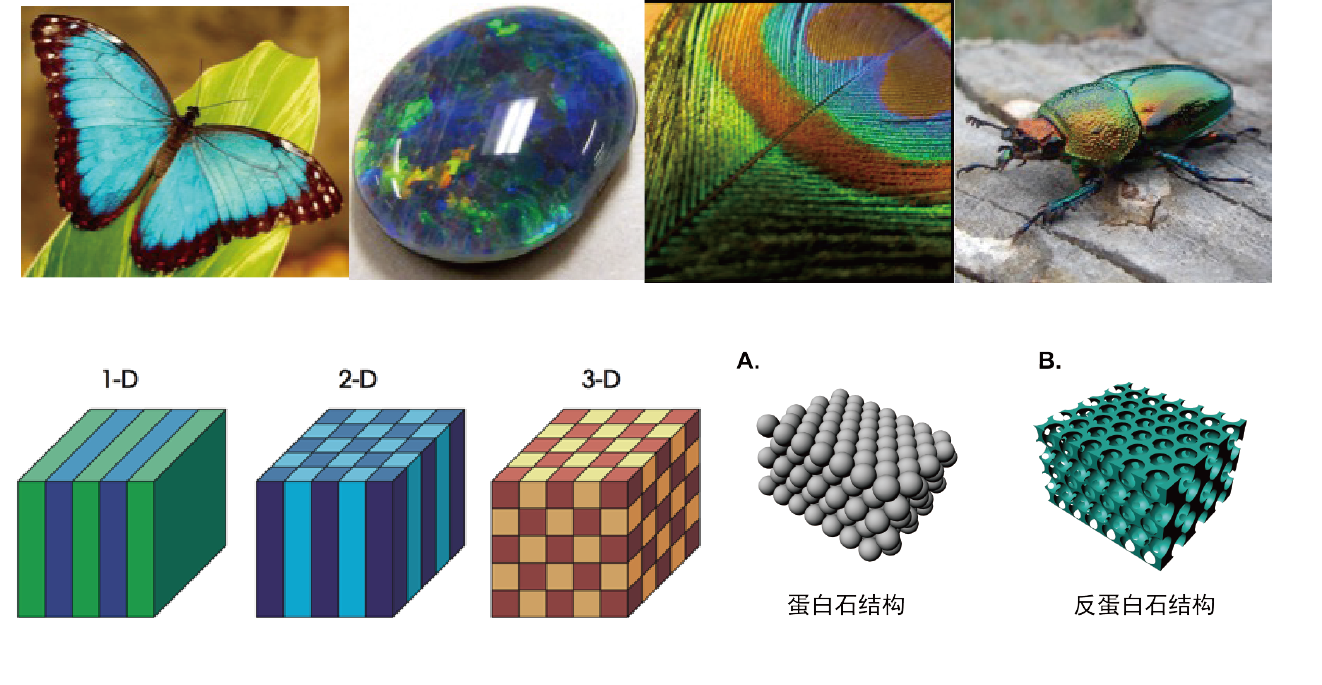
\includegraphics[width=10cm]{figures/PhC.png}
  \end{center}
  % \pause
  光子禁带:光子晶体结构对特定频域内的光的调制(传播受限)
\end{frame}

\begin{frame}
  \frametitle{光子晶体原理}
  \begin{minipage}{0.48\textwidth}
    光子晶体禁带性质:
    \begin{equation*}
      m\lambda=2d\sqrt{\sum_{i}n_i^2f_i-sin^2\theta}
    \end{equation*}

    \pause

    % \begin{itemize}[<+-| alert@+>]
    \begin{itemize}
      \item
      $\lambda$: 光子禁带的中心波长
      \item
      \large $d$: 光子晶体晶格常数
      \item
      $n_i$: 光子晶体各组分折射率
      \item
      $\theta$: 入射光角度
    \end{itemize}
  \end{minipage}
  \hfill
  \pause
  \begin{minipage}{0.5\textwidth}
    光子禁带的调制
    \begin{center}
      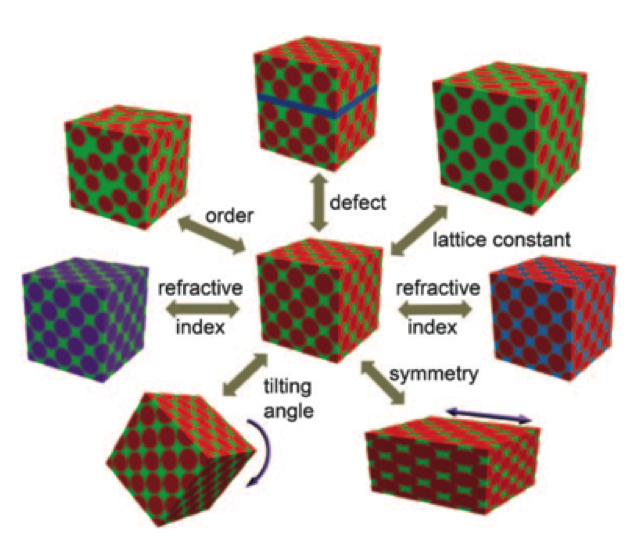
\includegraphics[width=\linewidth]{figures/PhC_control.png}
    \end{center}
  \end{minipage}
\end{frame}
  
% \begin{frame}
%   \frametitle{光子晶体在传感中的应用}
%   \begin{minipage}{0.48\textwidth}
%     \tiny 离子与pH响应
%     \begin{figure}[htbp]
%       \begin{center}
%       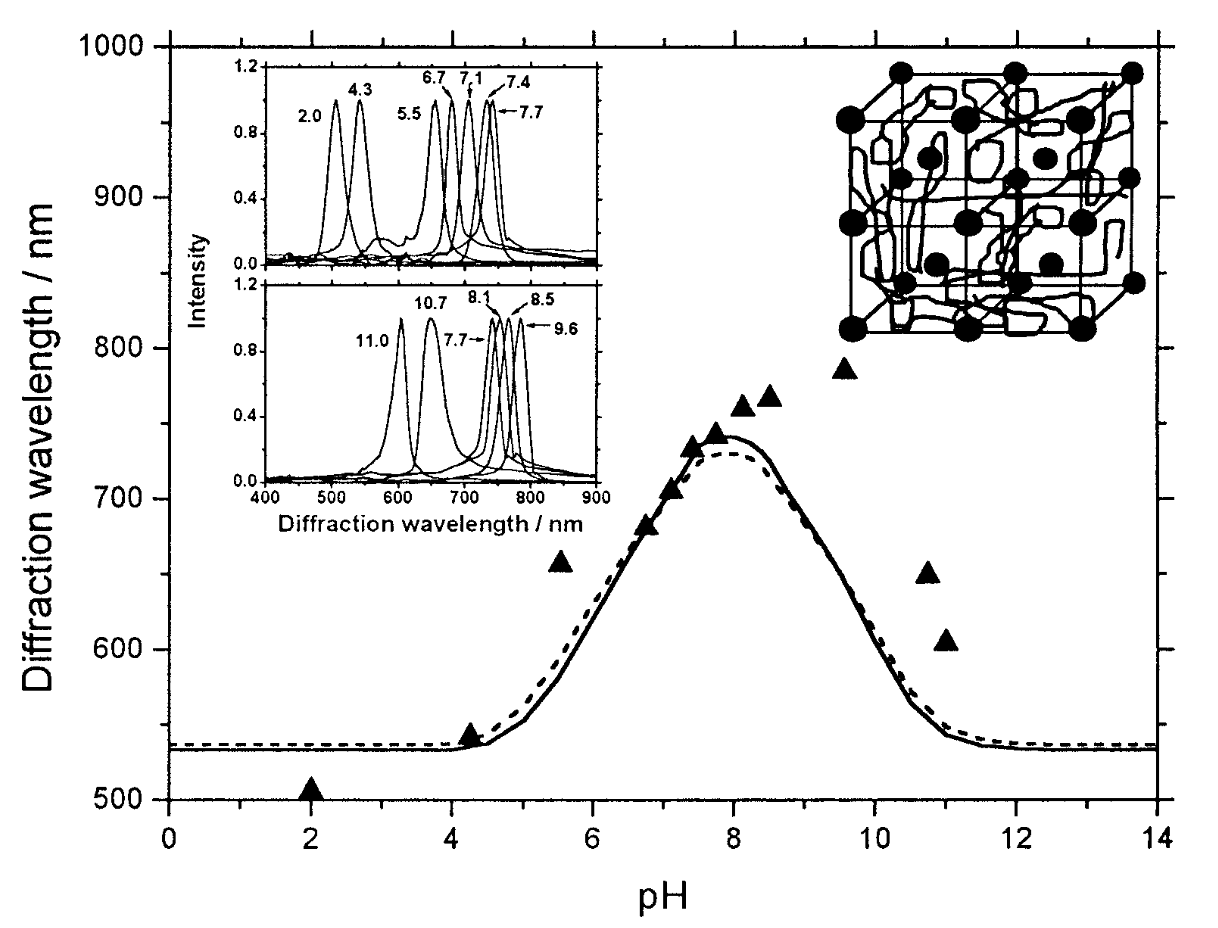
\includegraphics[height=0.4\linewidth]{figures/asher-ph.png}
%       \end{center}
%     \end{figure}
%   \tiny Lee et al. \textit{J. Am. Chem. Soc. }\textbf{2000}, 122, 9534–9537.\\
%     分子印迹识别
%     \begin{figure}[htbp]
%         \begin{center}
%         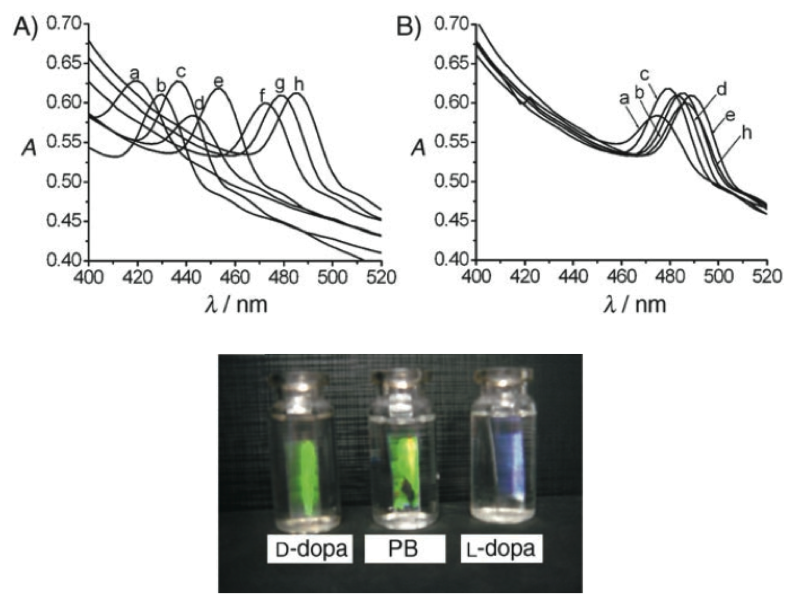
\includegraphics[height=0.4\linewidth]{figures/huxiaobin.png}
%         \end{center}
%     \end{figure}

%     \tiny Hu et al. \textit{Angew. Chem.} \textbf{2006}, 45, 8145–8148.
%   \end{minipage}
%   \hfill
%   \begin{minipage}{0.5\textwidth}
%     \tiny 温度传感
%     \begin{figure}[htbp]
%       \begin{center}
%         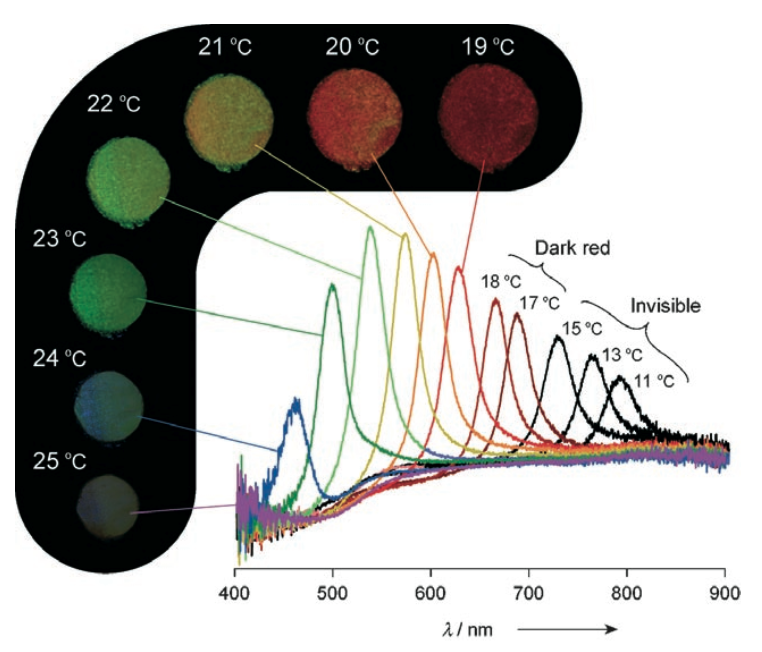
\includegraphics[height=0.4\linewidth]{figures/watanabe.png}
%         \end{center}
%     \end{figure}
%     \tiny Matsubara, et al. \textit{Angew. Chem.}, \textbf{2007}, 119, 1718–1722.\\
%     \tiny 压力传感
%     \begin{figure}[htbp]
%       \begin{center}
%         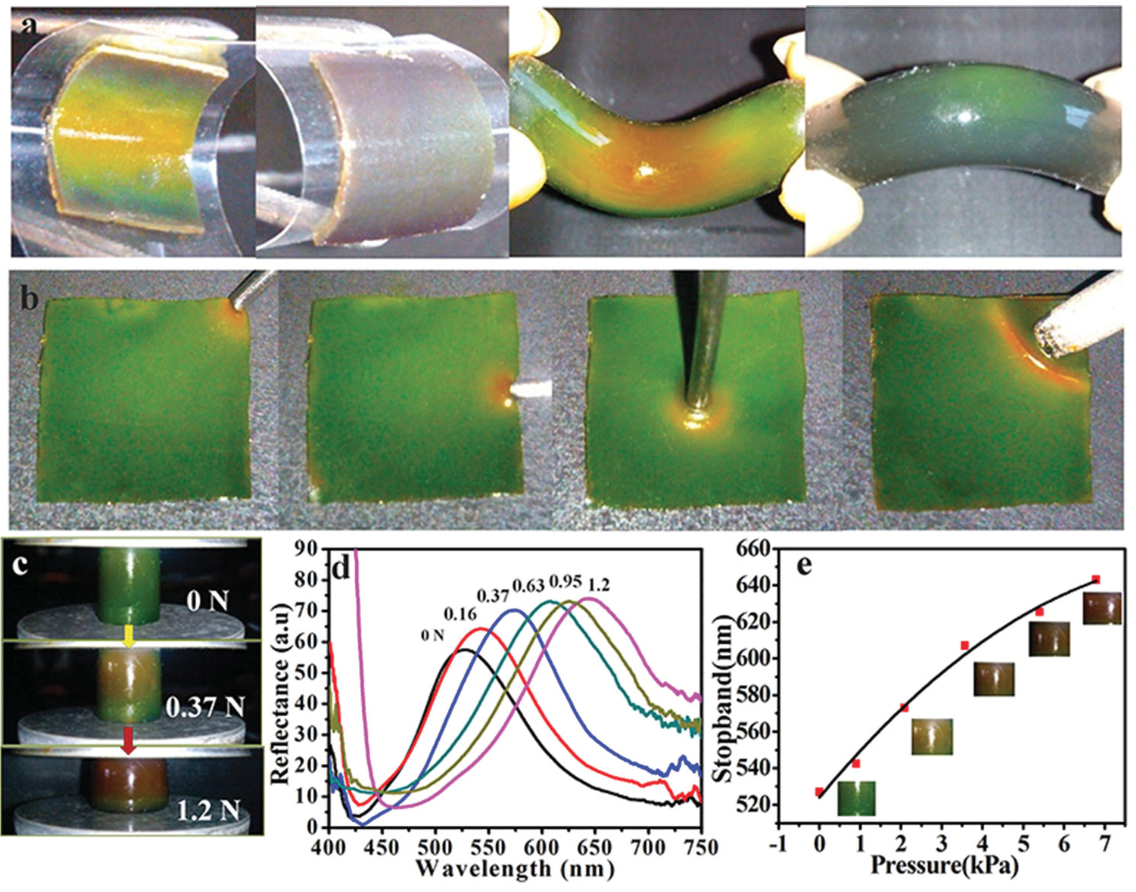
\includegraphics[height=0.38\linewidth]{figures/chensu.png}
%         \end{center}
%     \end{figure}
%     \tiny Wang, et al. \textit{Adv. Opt. Mater.} \textbf{2014}, 10.1002/adom.201300538.

%   \end{minipage}
% \end{frame}

\begin{frame}
  \frametitle{基于化学反应的光子晶体材料}
  \begin{figure}[htbp]
    \centering
    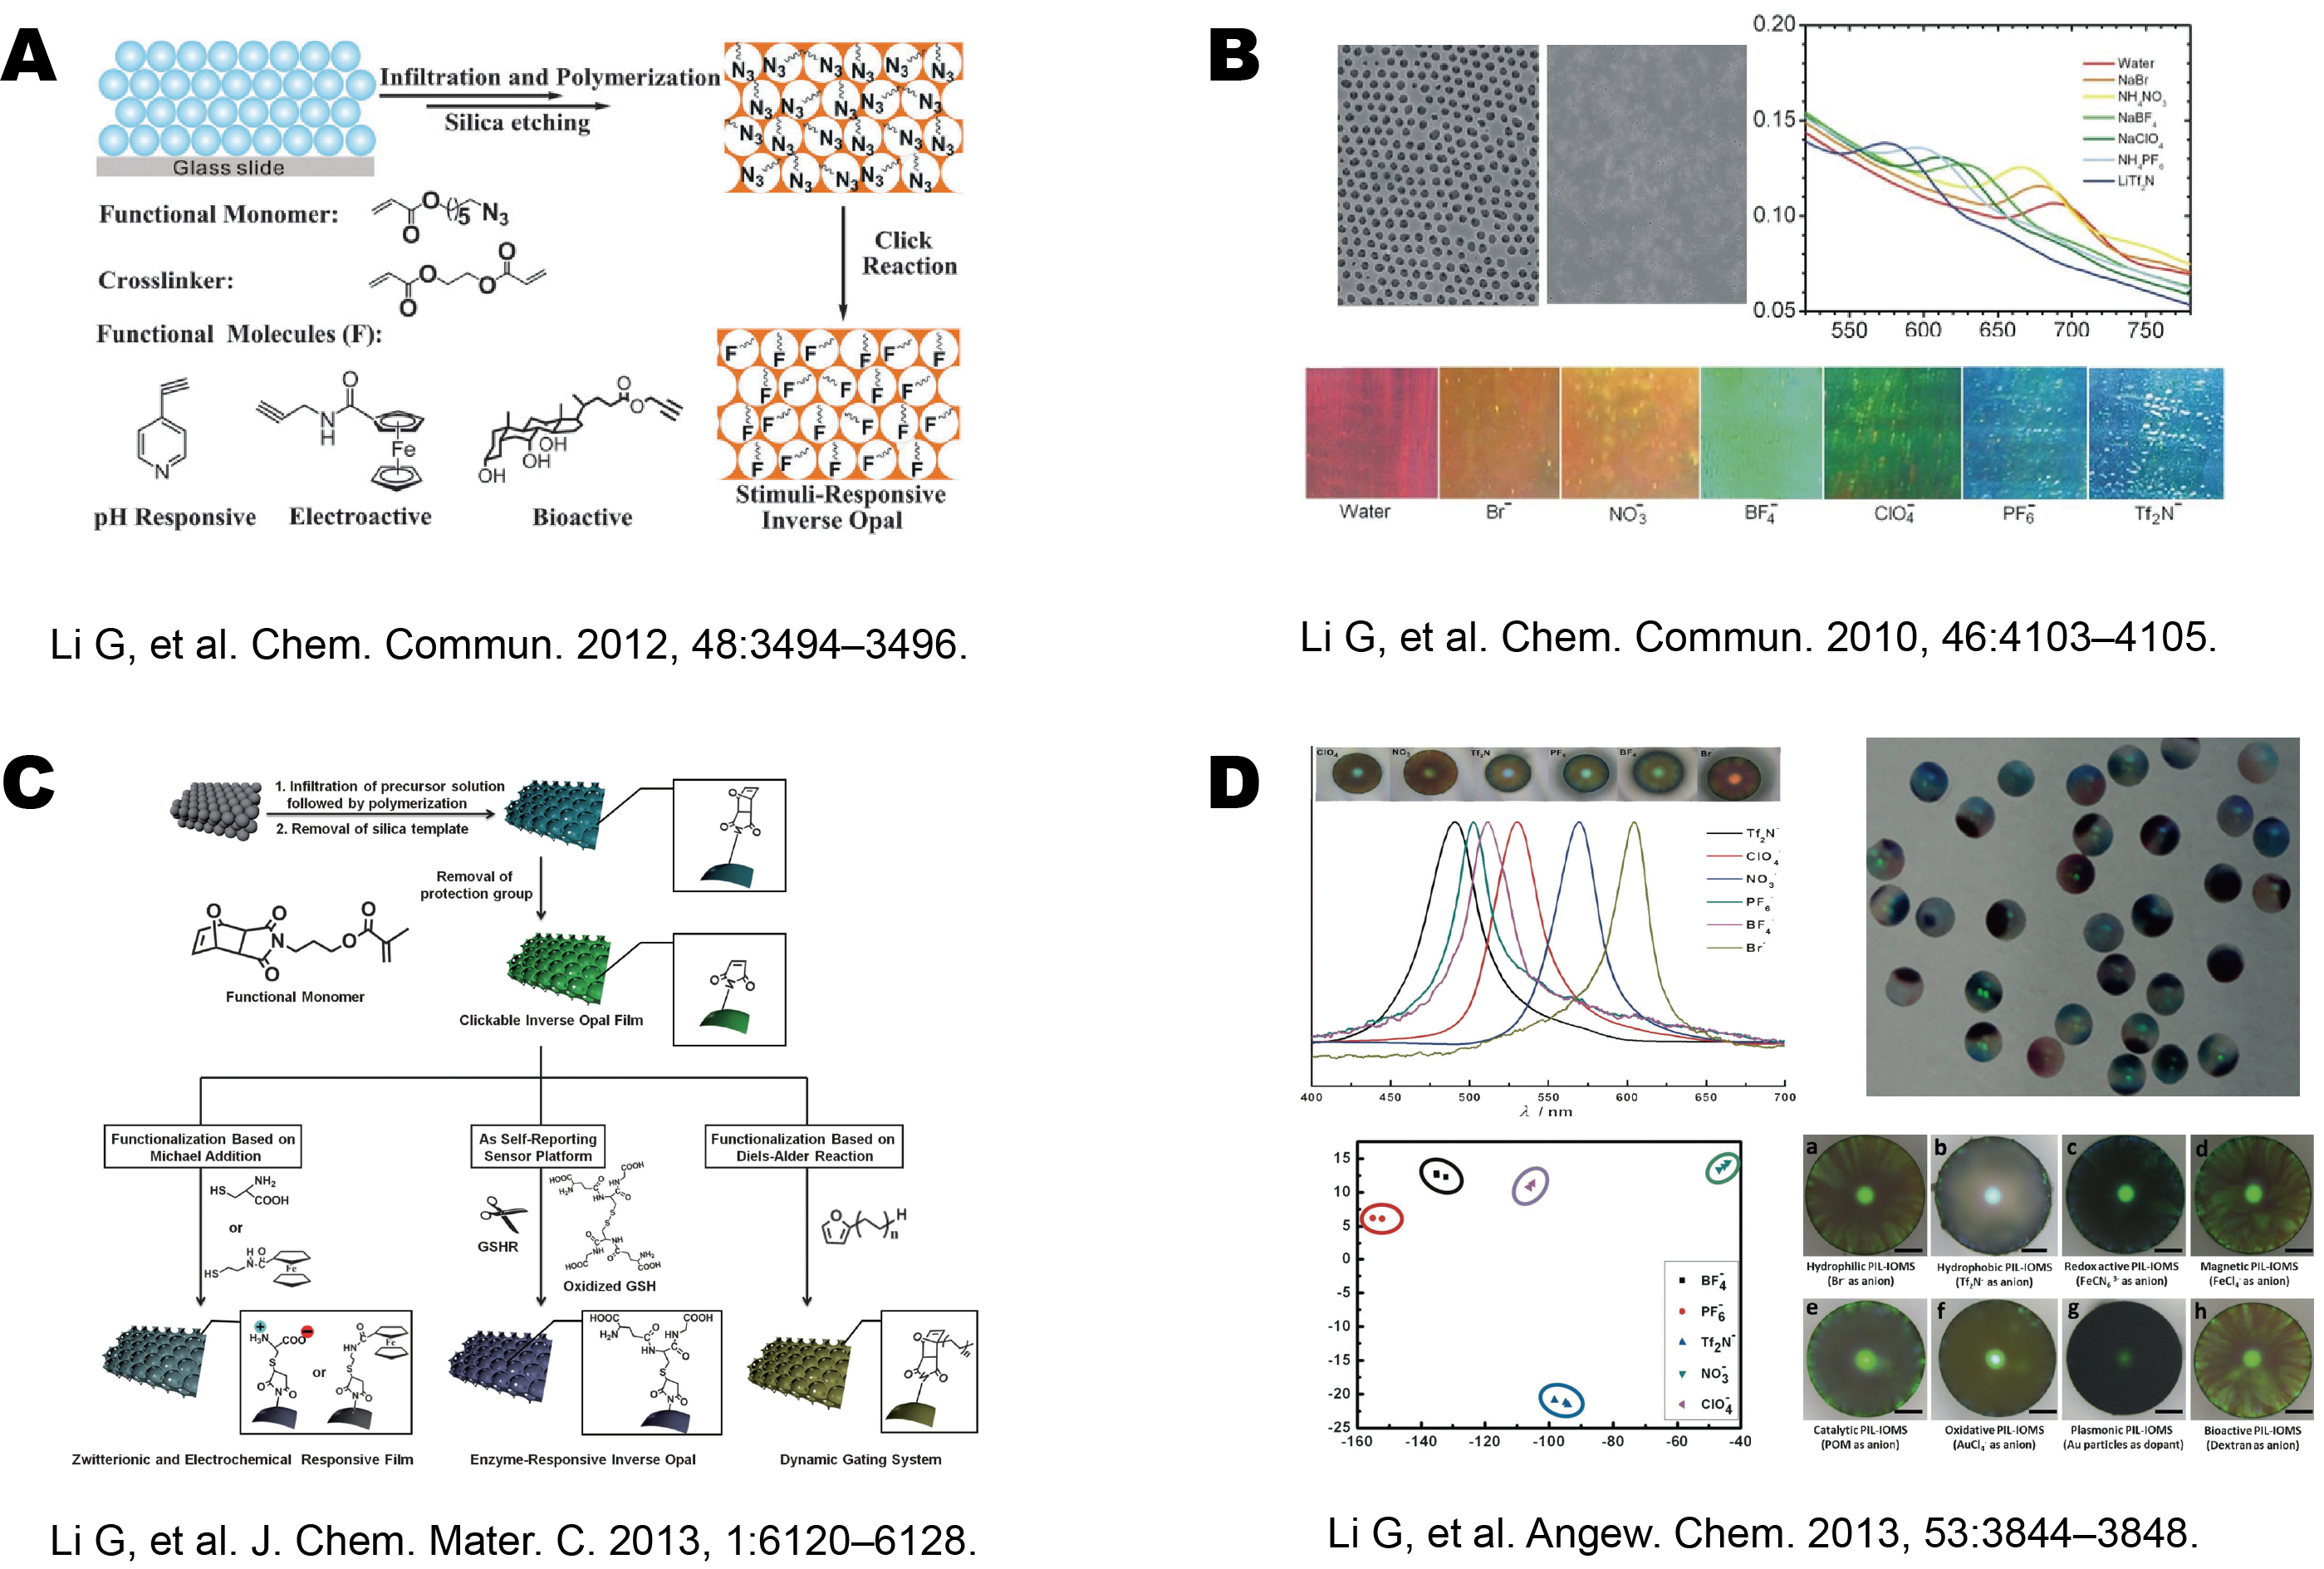
\includegraphics[width=0.90\linewidth]{figures/chem-react.png}
  \end{figure}
\end{frame}

% \begin{frame}
%   \frametitle{光子晶体图案化的研究}
%   \begin{figure}
%     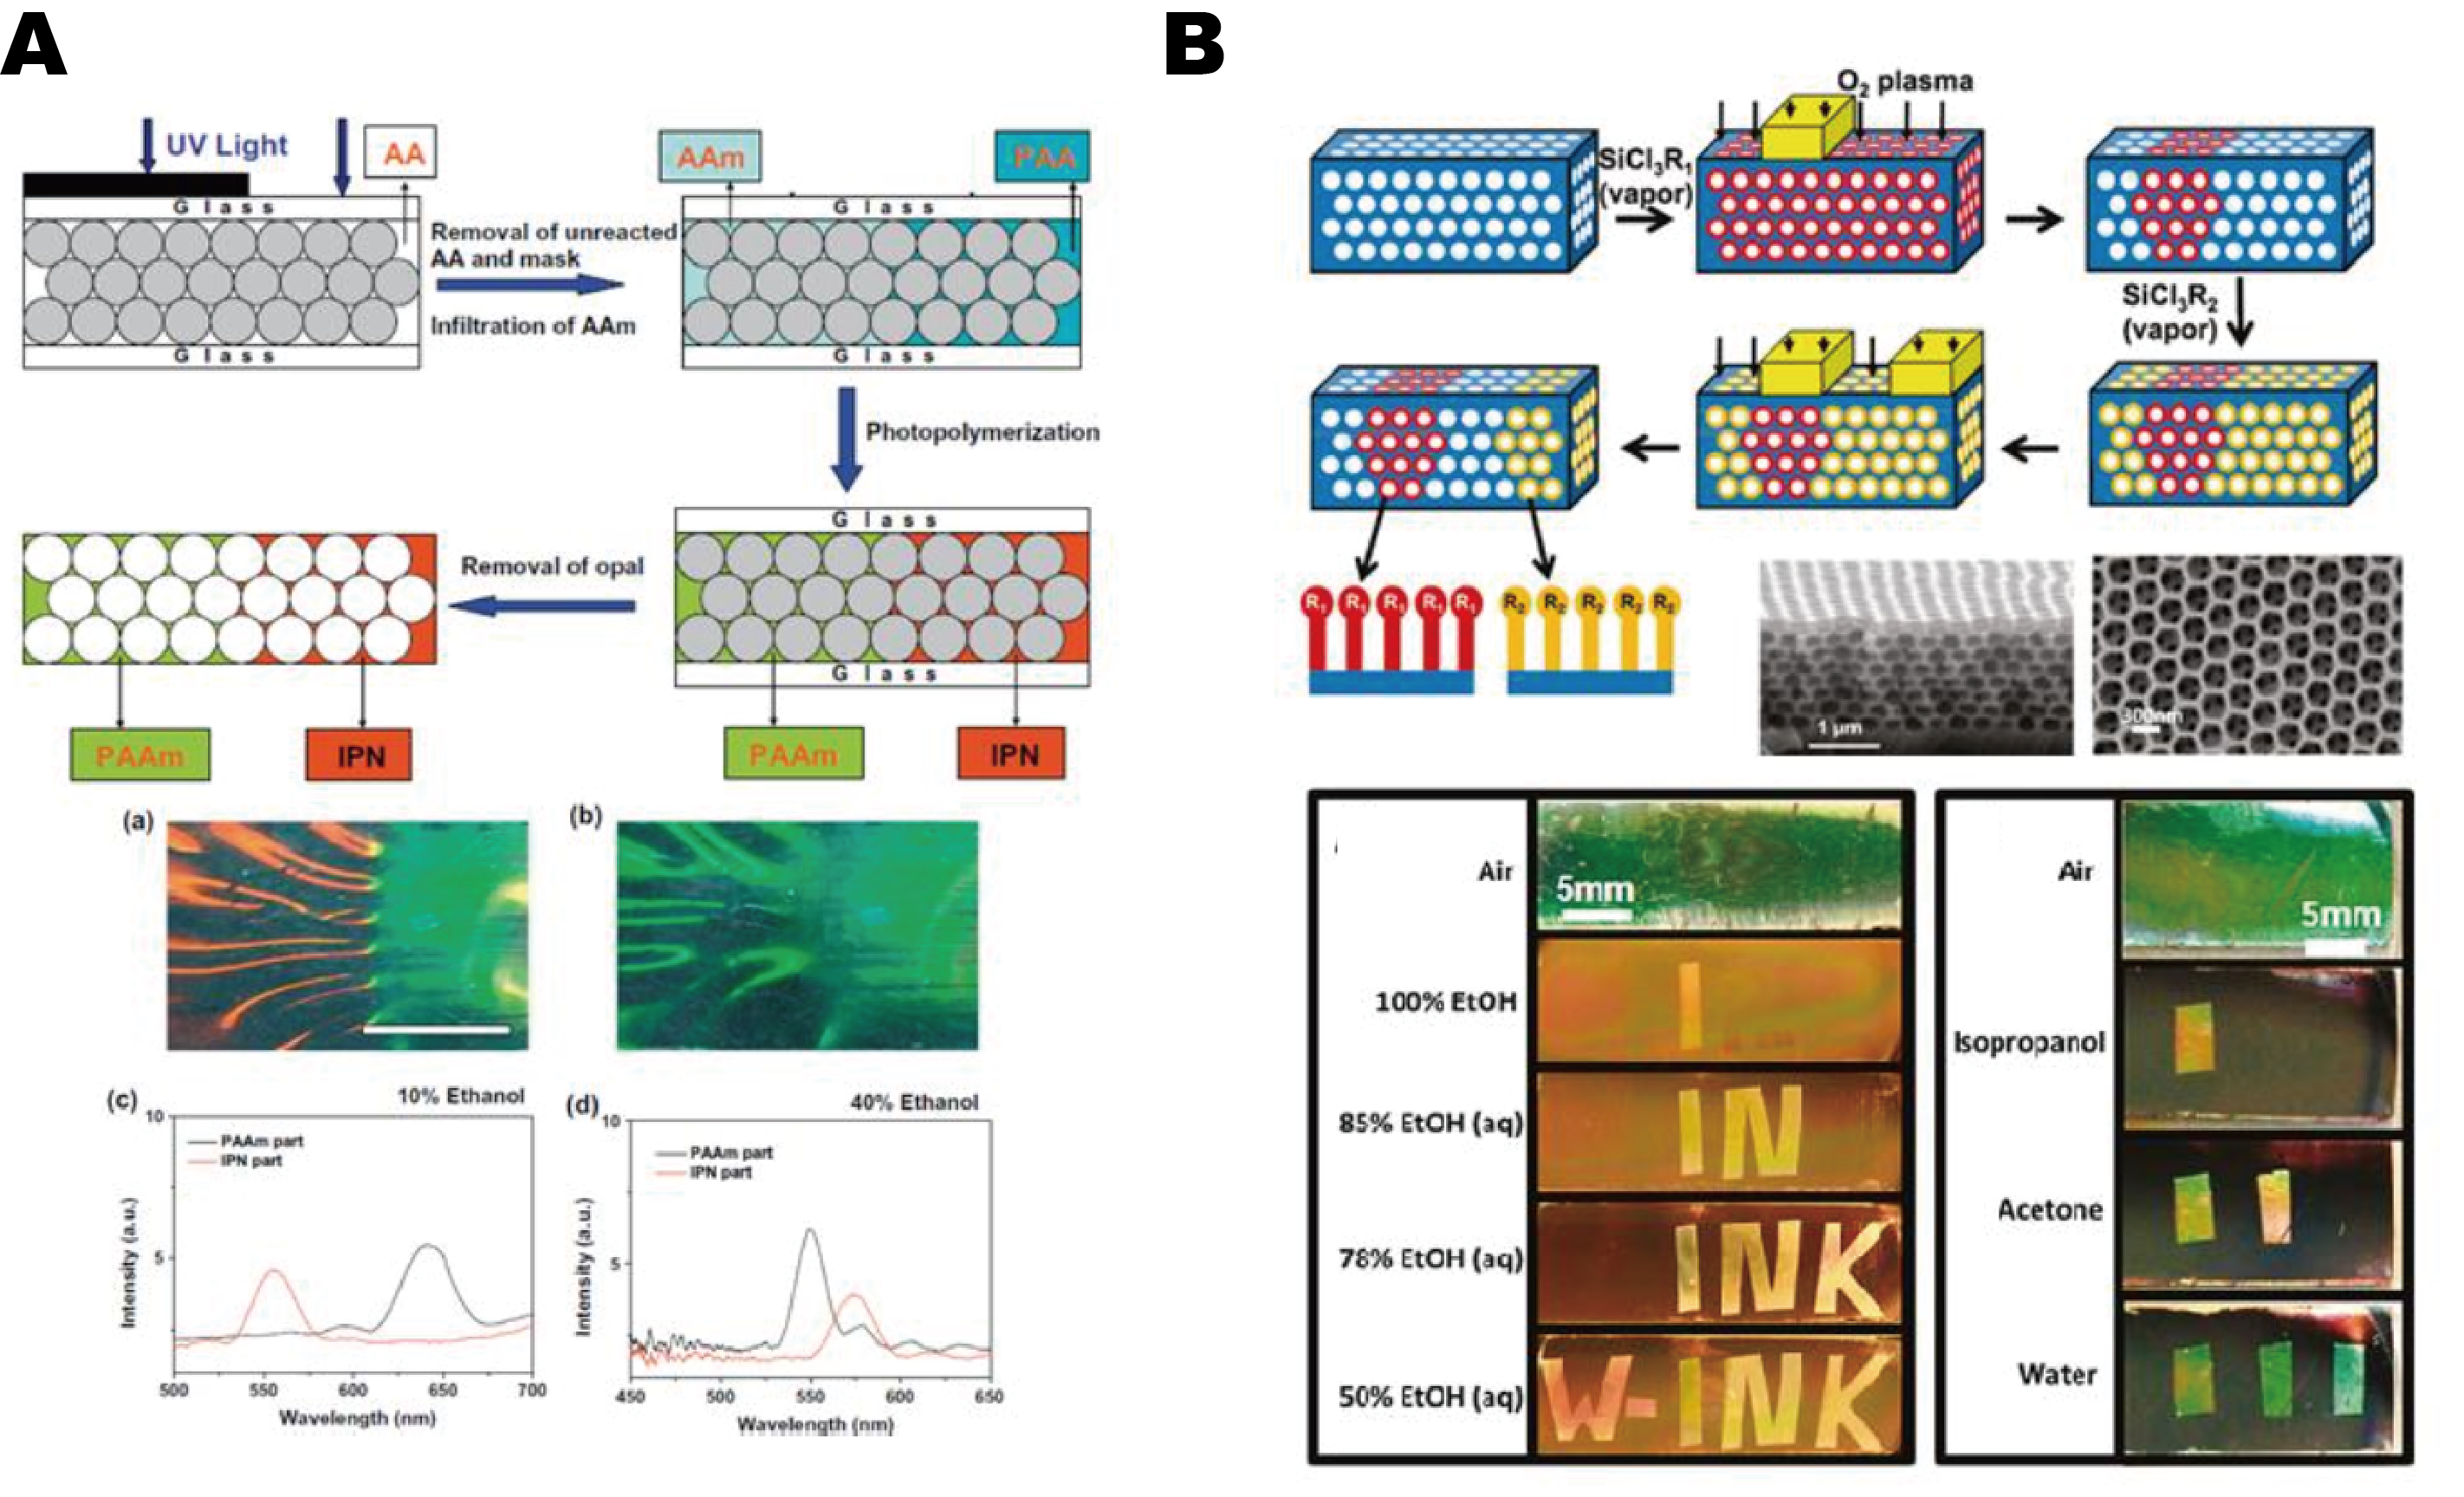
\includegraphics[=0.8\linewidth]{figures/inverse_opal_pattern.png}
%   \end{figure}
%   \tiny A. Wang, et al. \textit{J. Colloid. Inter. Sci.} \textbf{2011}, 353 , 498–505. B. Burgess, et al. \textit{J. Am. Chem. Soc.}  \textbf{2012}, 134 ), 1374–1374.
% \end{frame}

\begin{frame}
  \frametitle{光子晶体:机遇与挑战}
  \pause
  \textcolor{tsinghua}{\textbf{光子晶体材料的优势}}
  % \begin{itemize}[<+-| alert@+>]
    \begin{itemize}
    \item
    信号自表达、操作简便
    \item
    材料多样性
    \item
    多孔内部结构、响应快速
  \end{itemize}
  \pause
  \textcolor{tsinghua}{\textbf{光子晶体材料的挑战}}
  % \begin{itemize}[<+-| alert@+>]
    \begin{itemize}
    \item
    功能材料的设计与参数优化
    \item
    光子晶体拓展性
    \item
    复杂、层次化光子晶体材料制备
  \end{itemize}
\end{frame}

\begin{frame}
  \frametitle{本工作研究目标}
  \begin{enumerate}
    \item
     研究不同化学反应在光子晶体传感、修饰中的应用
    \item
     通过化学反应修饰,拓展光子晶体多样性
    \item
     基于化学反应制备具有复杂结构与化学组分的光子晶体材料
  \end{enumerate}
\end{frame}

\section{研究内容}

% \subsection{光子晶体模板制备}
% \begin{frame}
%   \frametitle{溶剂蒸发诱导的垂直沉积法制备三维光子晶体}
%   \begin{figure}[htbp]
%     \centering
%     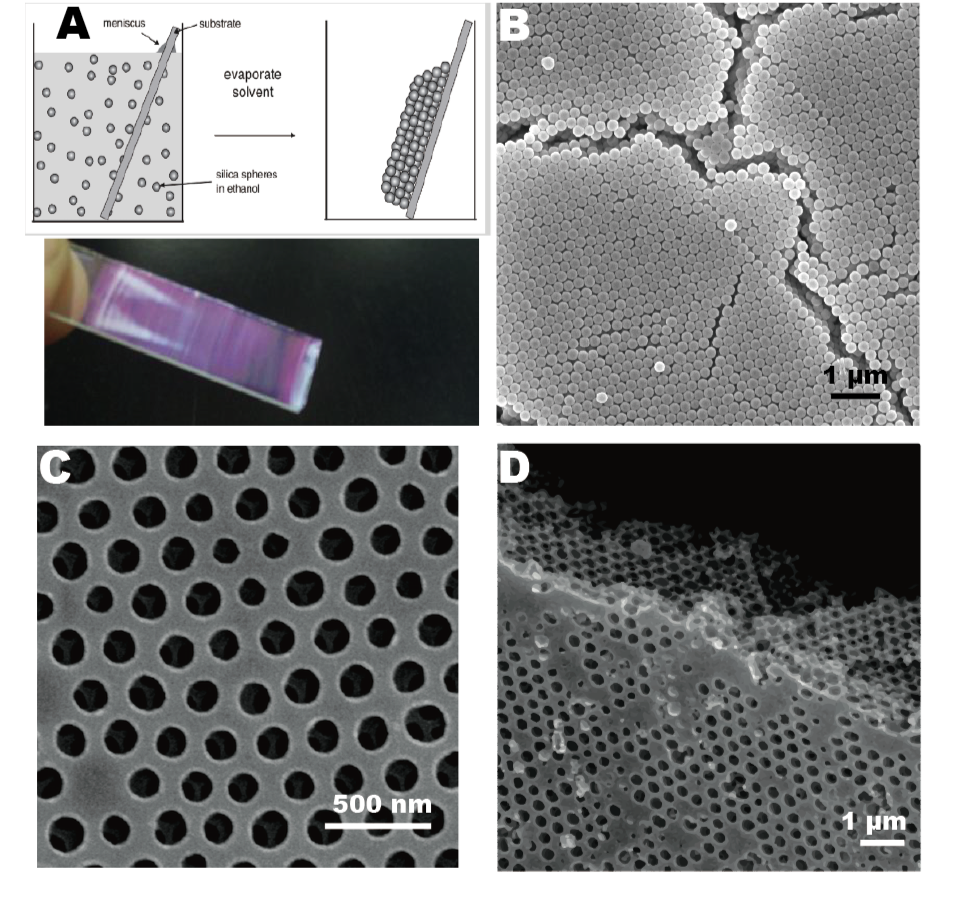
\includegraphics[height=0.60\linewidth]{figures/opal-eval.png}
%   \end{figure}
% \end{frame}

% \begin{frame}
%   \frametitle{LbL逐层堆积法制备三维光子晶体}
%   \begin{figure}[htbp]
%     \centering
%     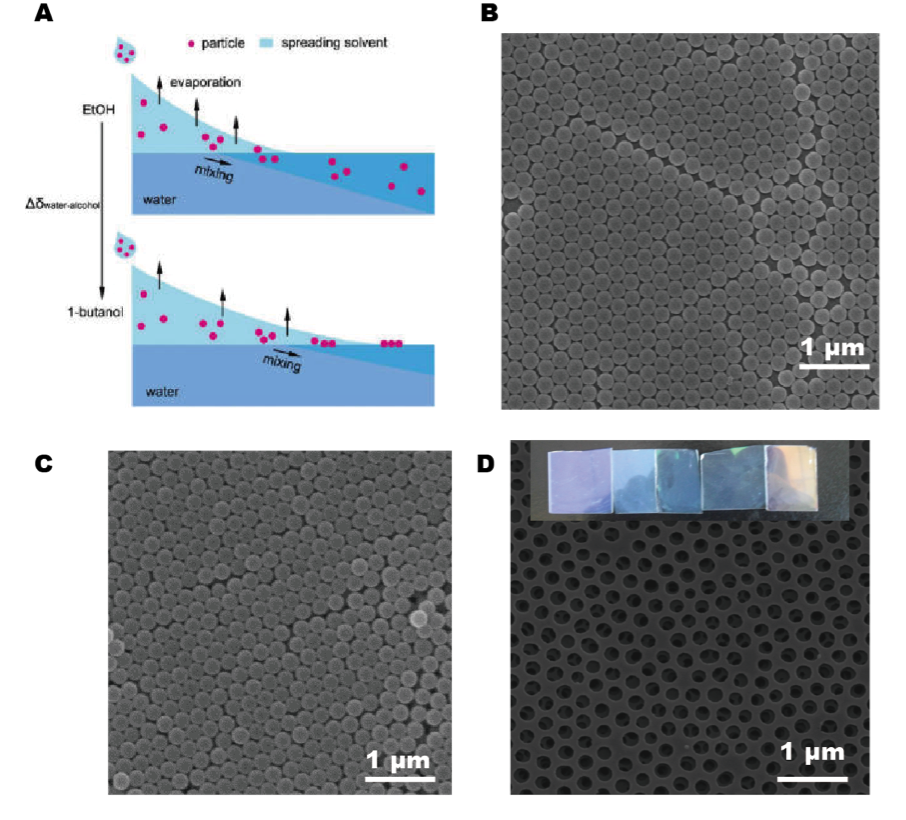
\includegraphics[height=0.60\linewidth]{figures/lbl.png}
%   \end{figure}
% \end{frame}

% \begin{frame}
%   \frametitle{微流控液滴法制备球形三维光子晶体}
%   \begin{figure}[htbp]
%     \centering
%     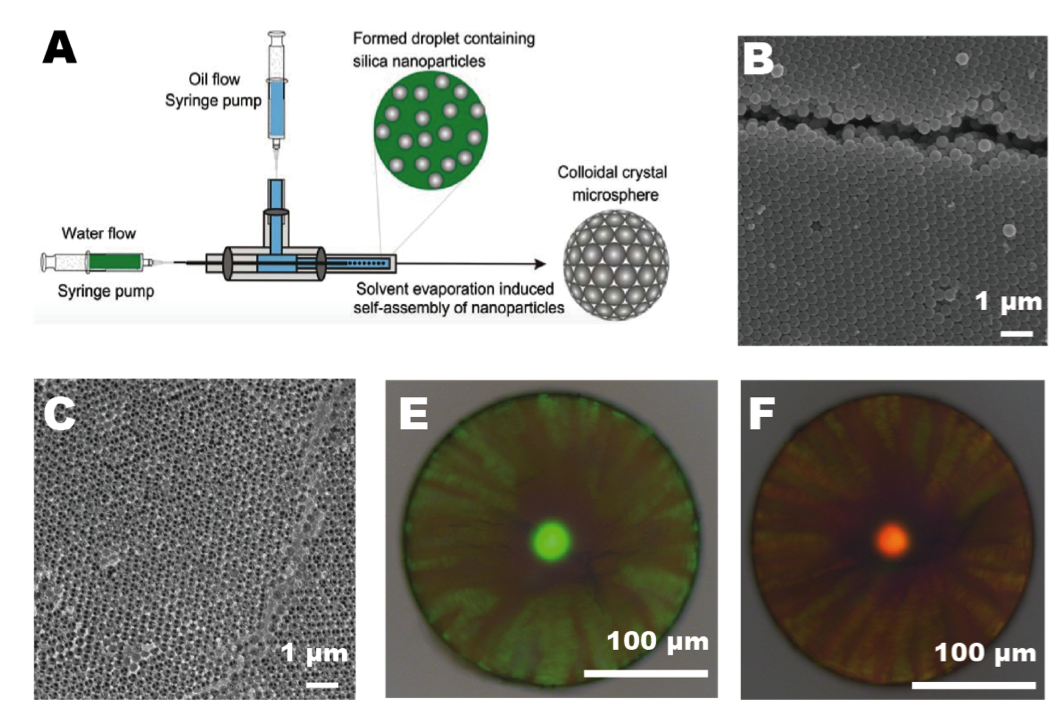
\includegraphics[height=0.60\linewidth]{figures/CCB.png}
%   \end{figure}
% \end{frame}

\subsection{基于马来酰亚胺的光子晶体乙酰胆碱酯酶活性检测的研究}
\begin{frame}
  \frametitle{实验原理}
  \begin{figure}[htbp]
    \centering
    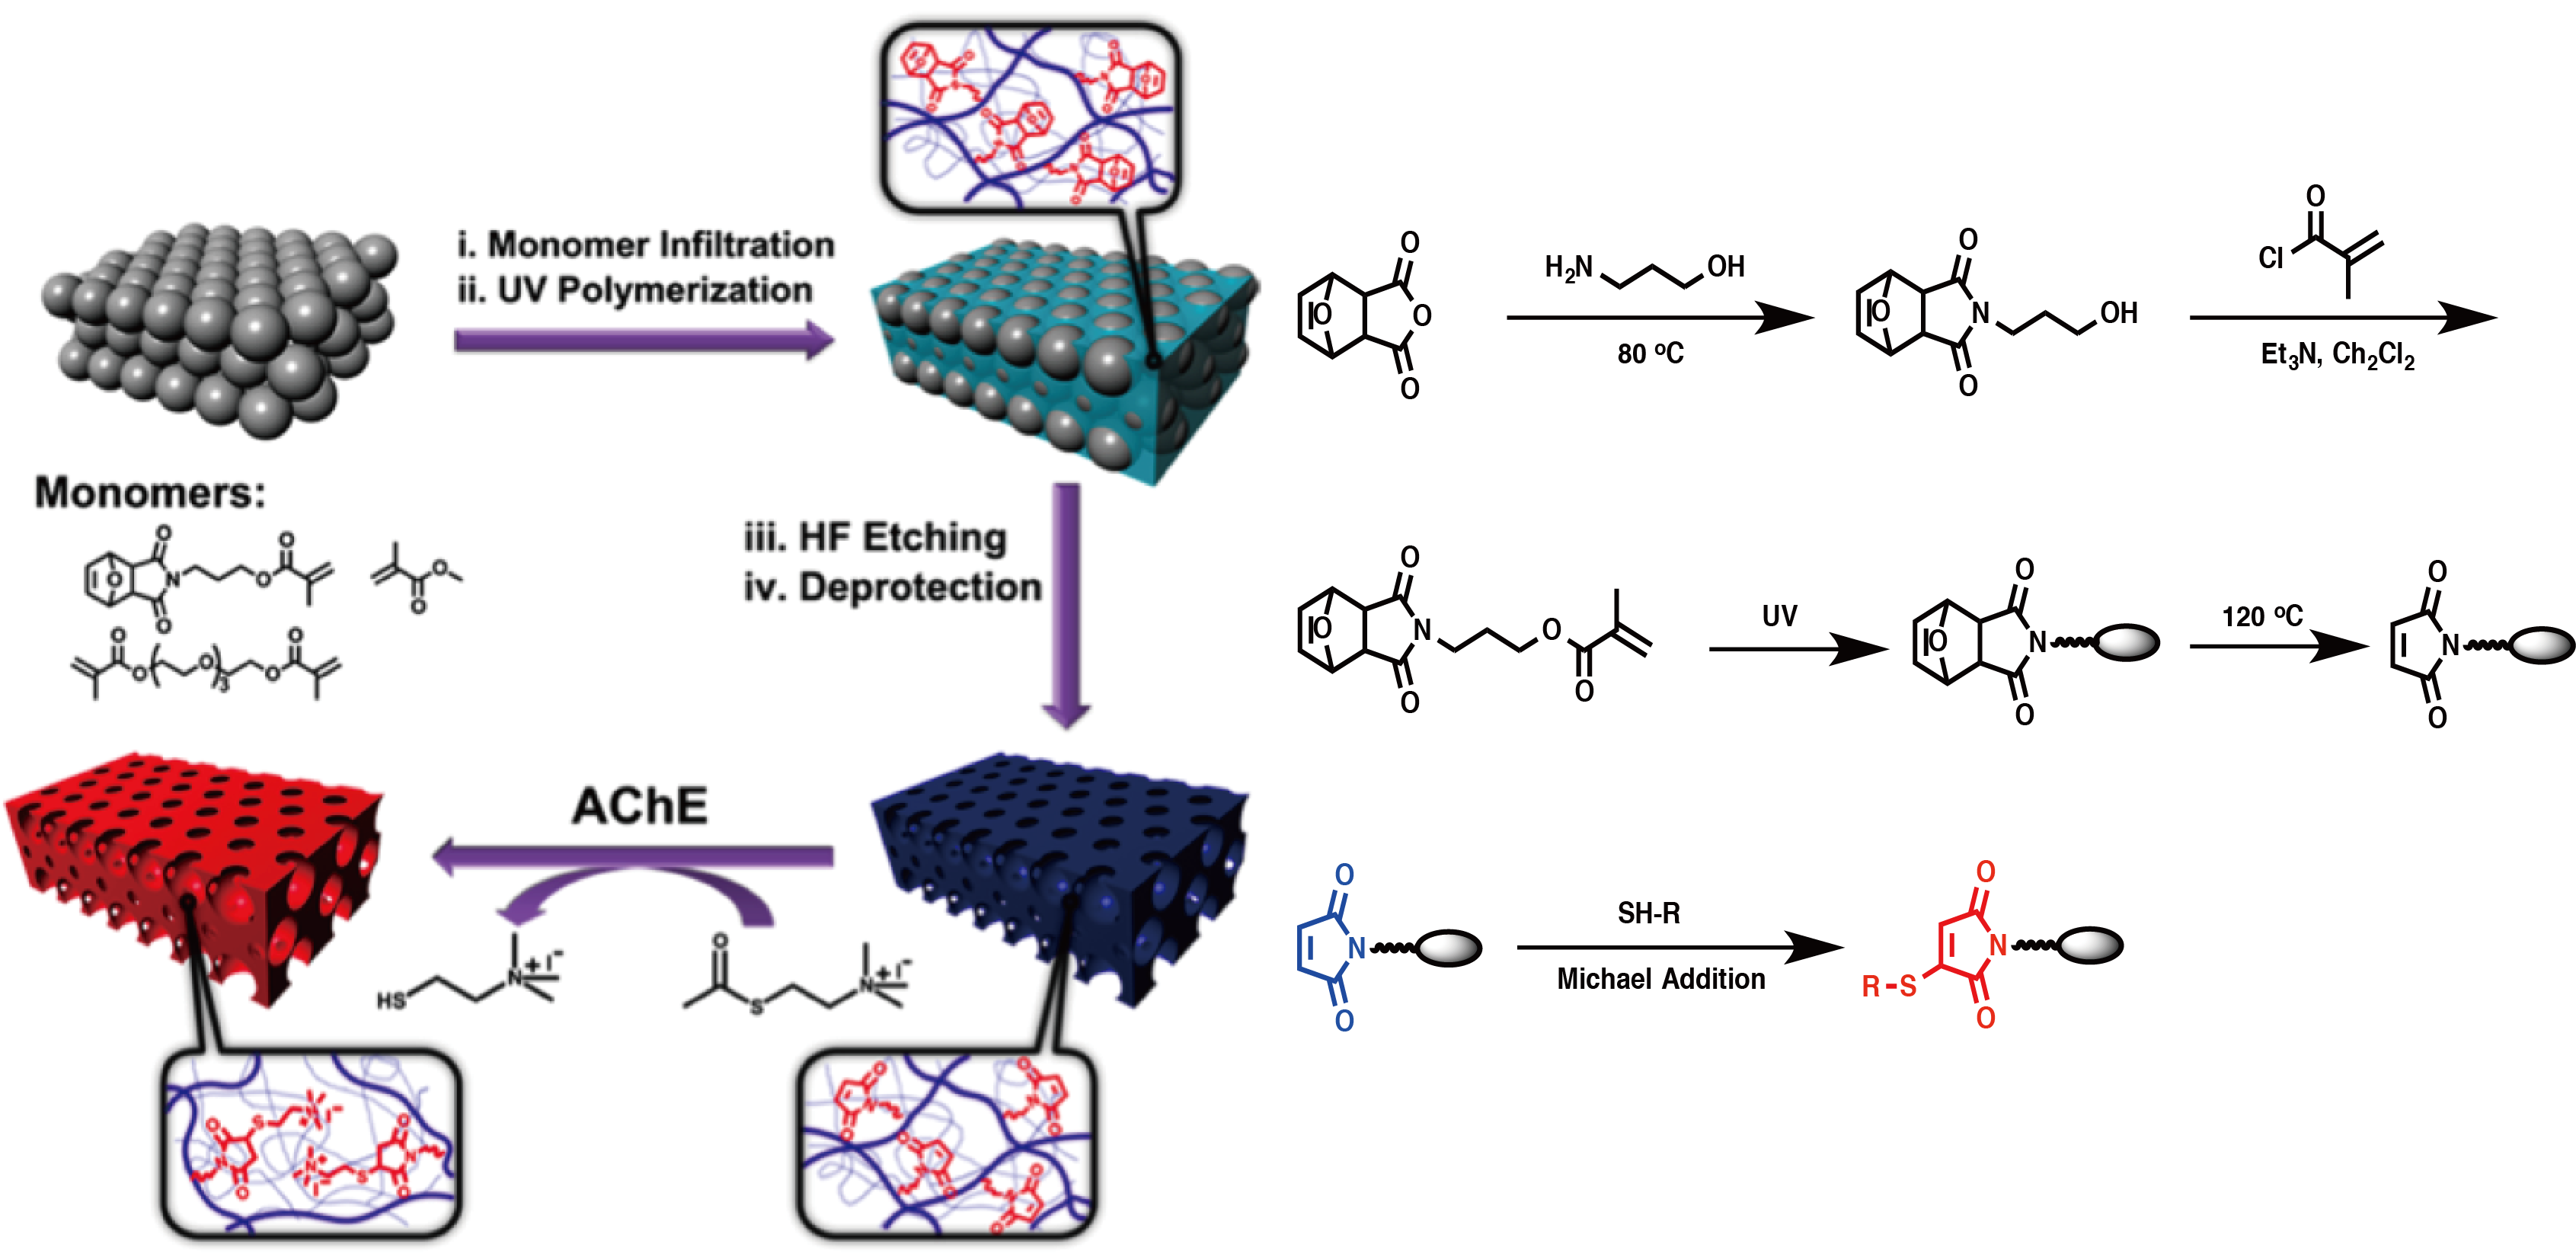
\includegraphics[width=\linewidth]{figures/AChE-Principle.png}
  \end{figure}
\end{frame}

\begin{frame}
  \frametitle{材料制备与表征}
  \begin{figure}[htbp]
    \centering
    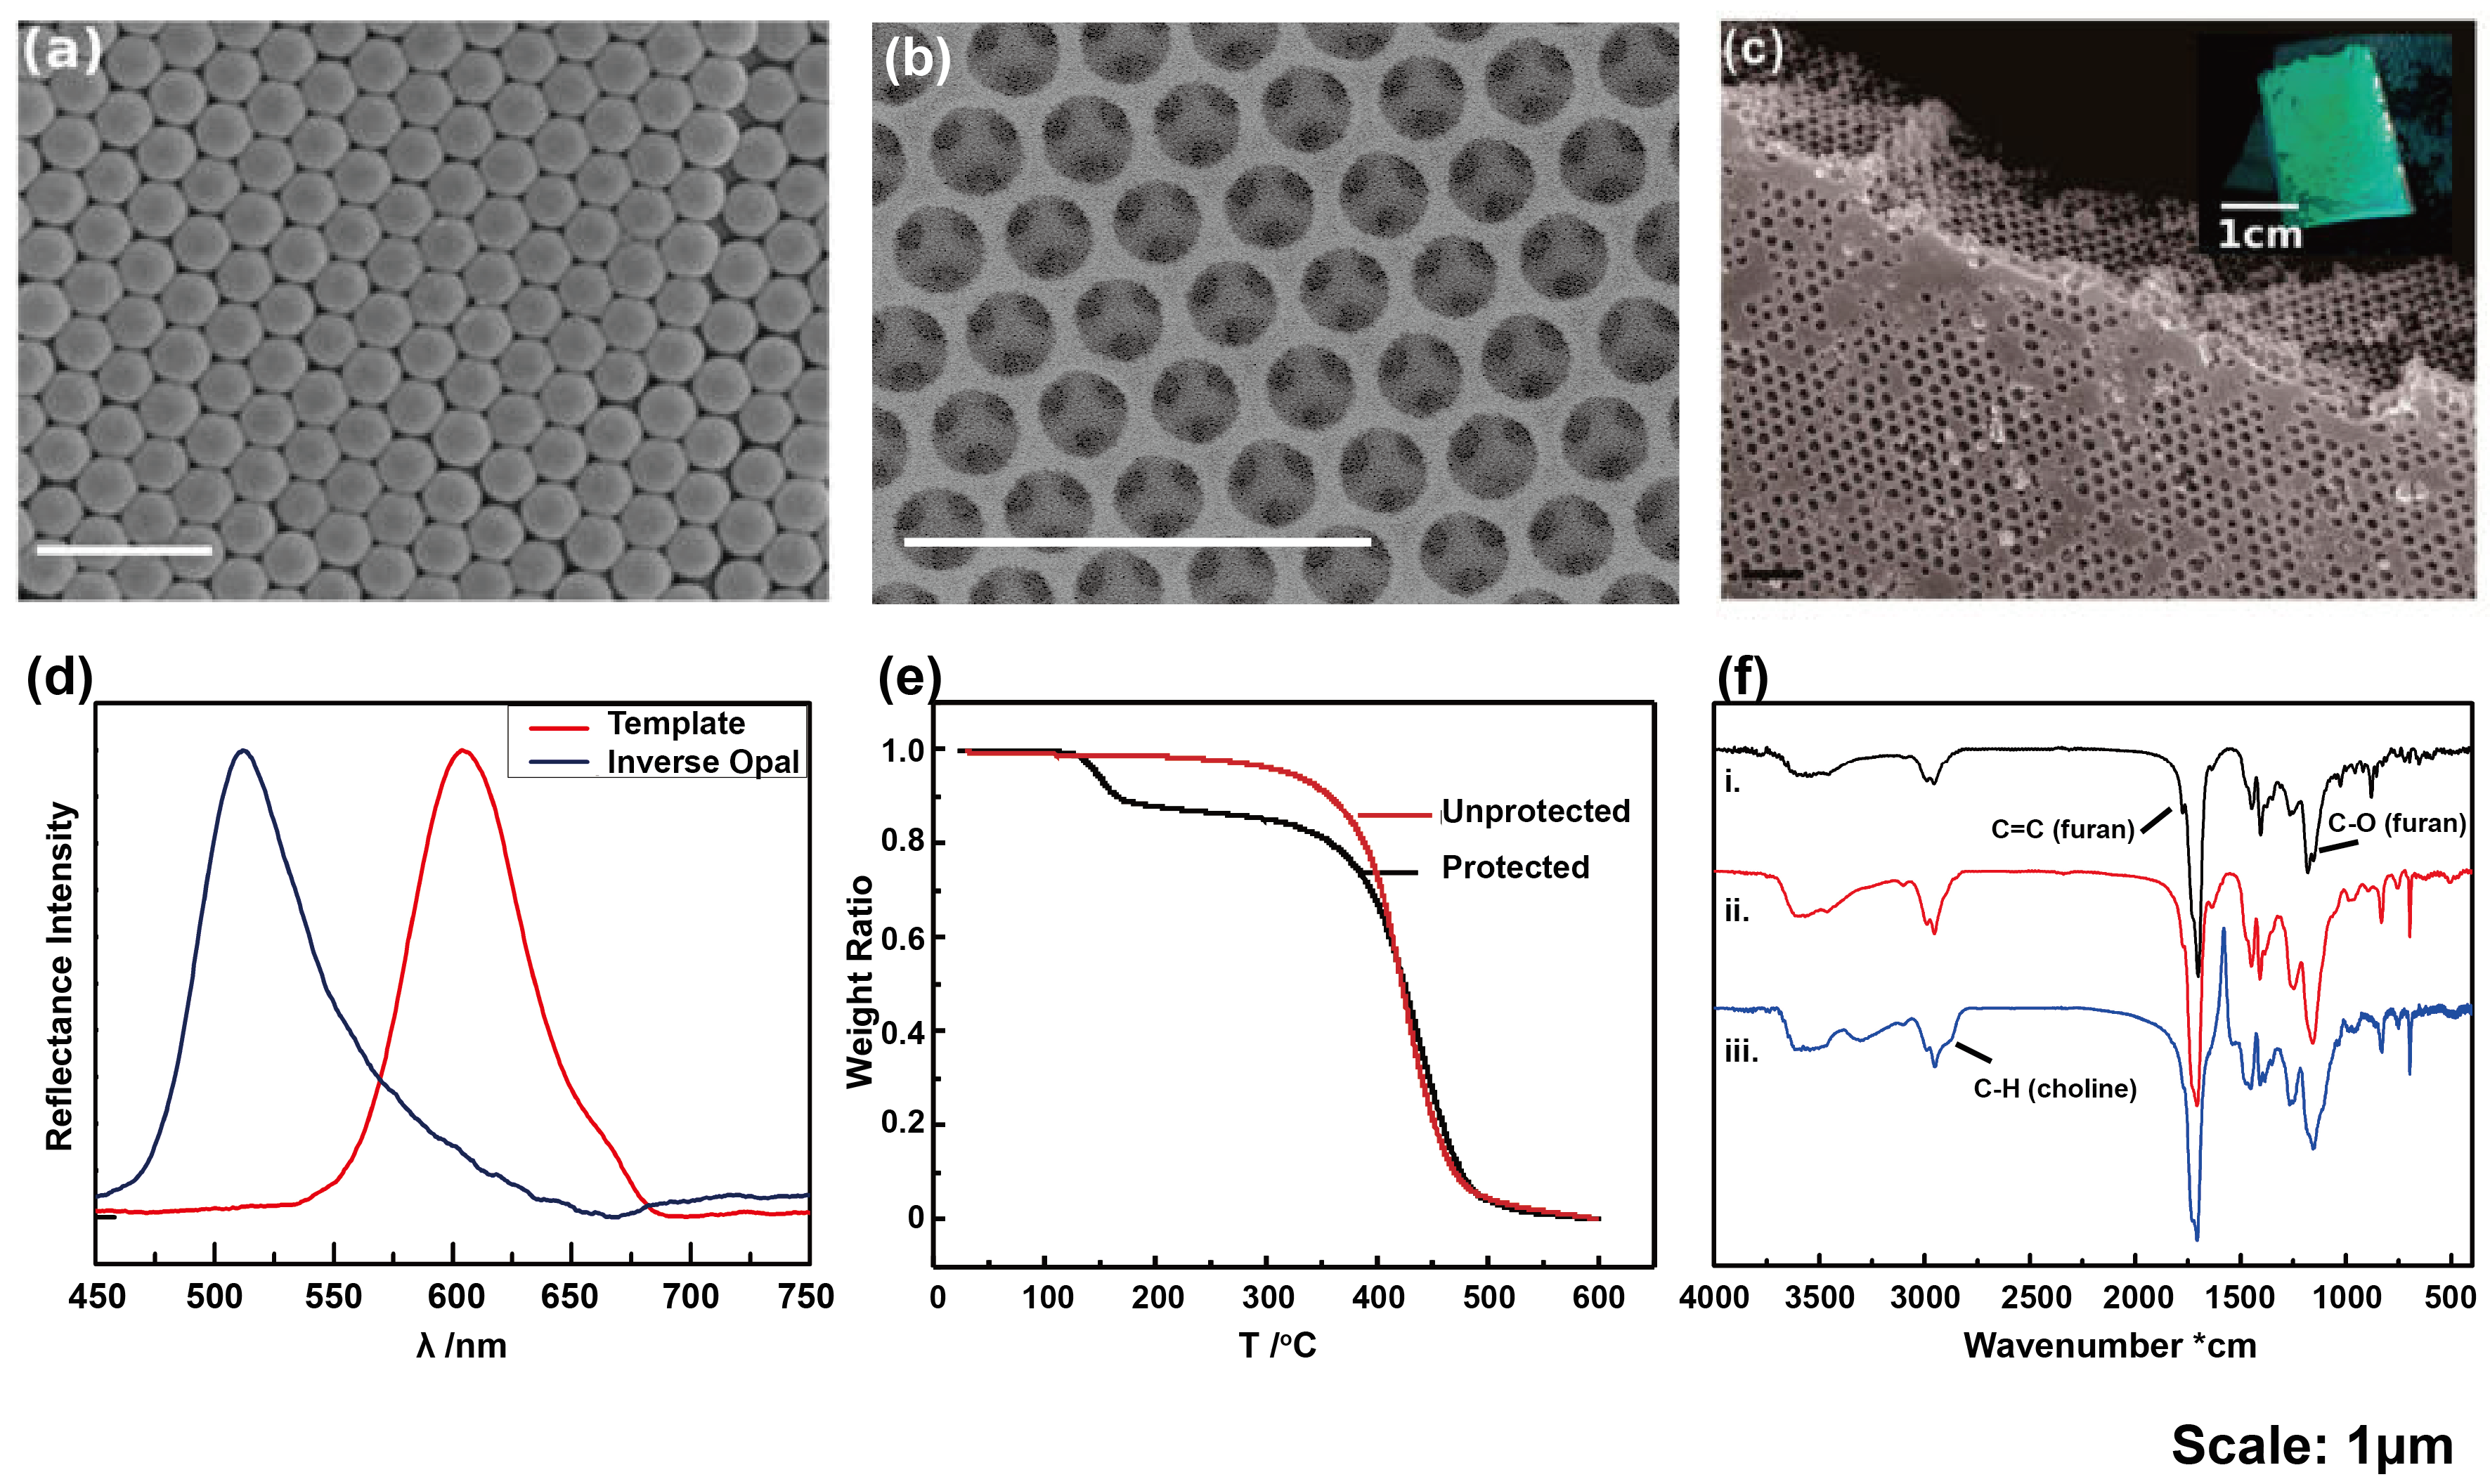
\includegraphics[width=\linewidth]{figures/ch2-chara.png}
  \end{figure}
\end{frame}


\begin{frame}
  \frametitle{对酶活性检测的灵敏性}
  \begin{figure}[htbp]
    \centering
    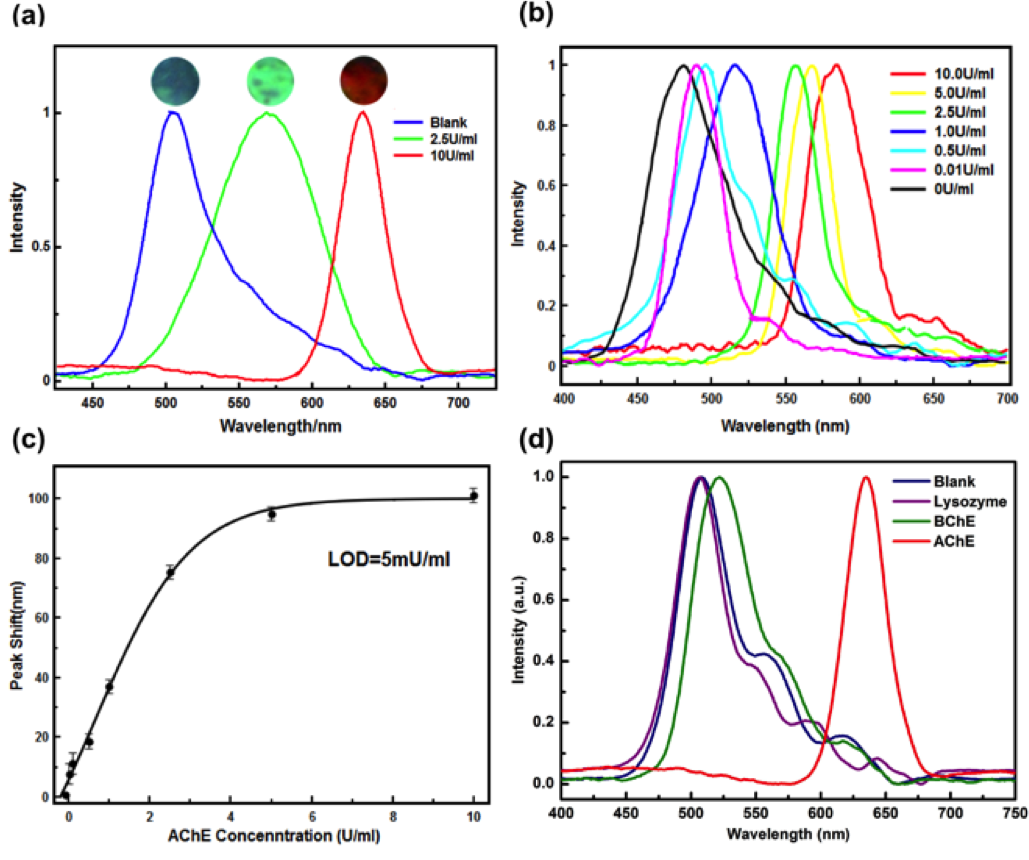
\includegraphics[height=0.60\linewidth]{figures/enzyme_sensitivity.png}
  \end{figure}
\end{frame}

\begin{frame}
  \frametitle{对酶动力学参数的检测}
  \begin{figure}[htbp]
    \centering
    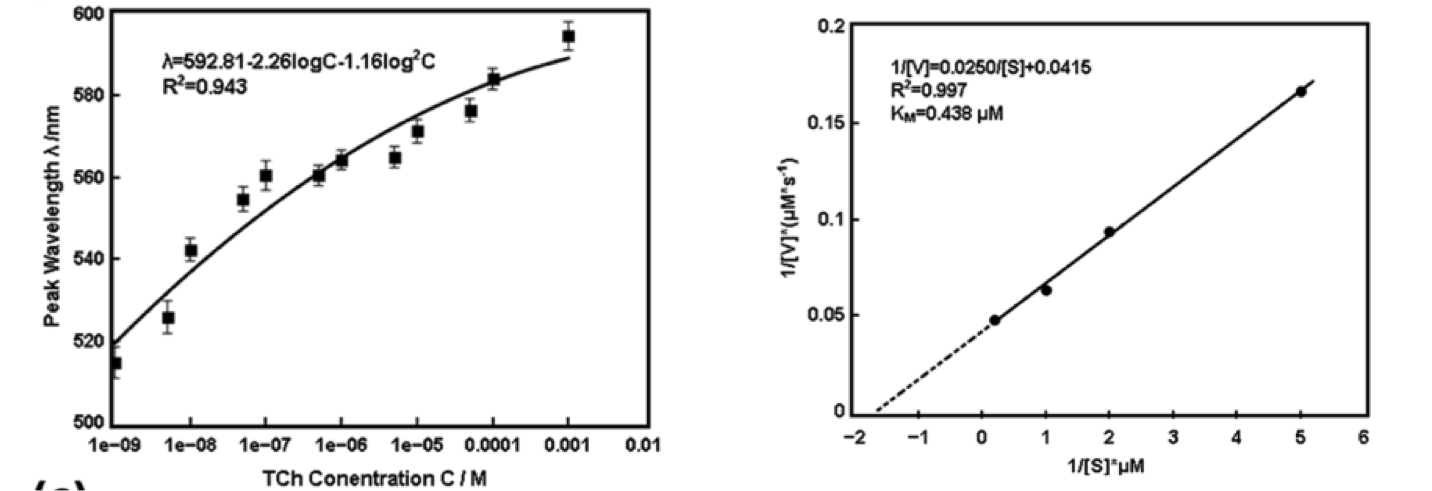
\includegraphics[width=\linewidth]{figures/kinetics.png}
  \end{figure}
\end{frame}

\begin{frame}
  \frametitle{对乙酰胆碱酶抑制剂的筛选}
  \begin{figure}[htbp]
    \centering
    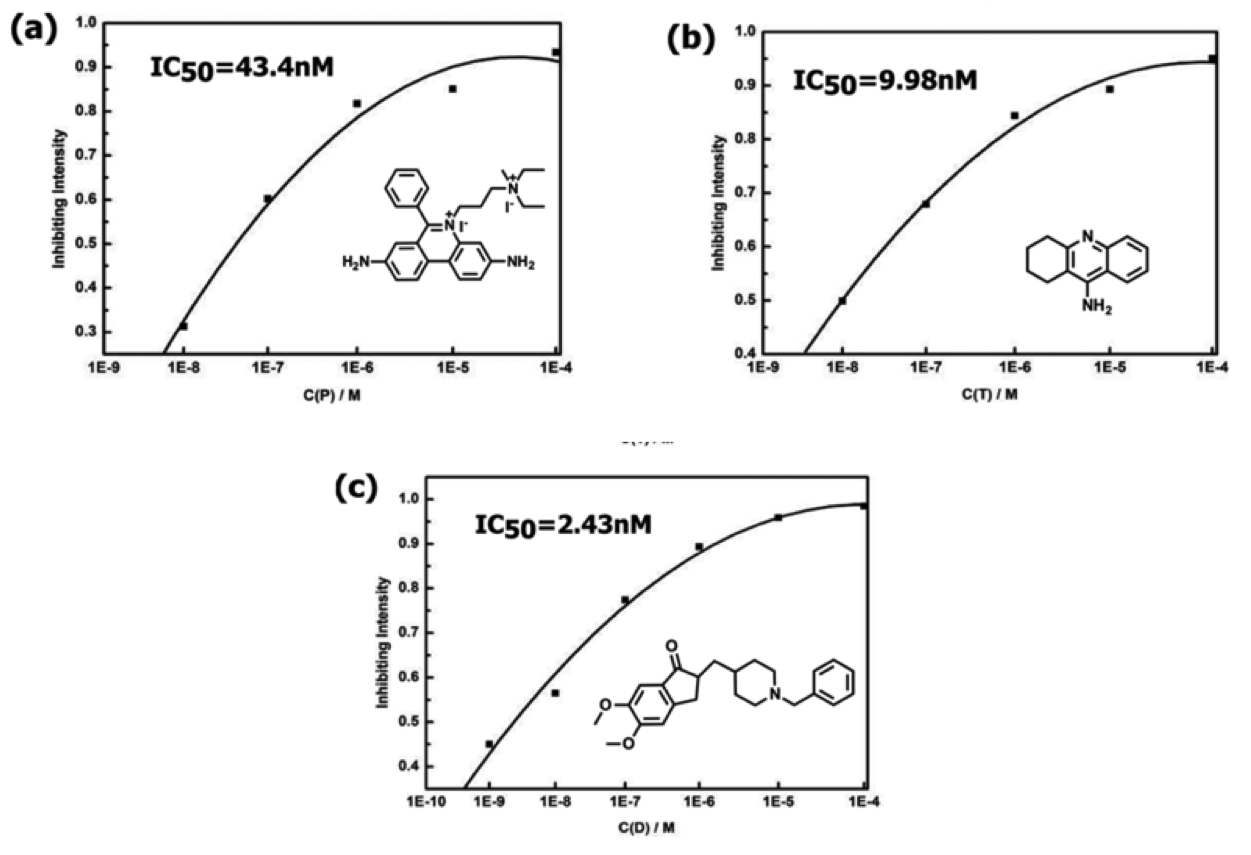
\includegraphics[width=0.85\linewidth]{figures/inhibitor.png}
  \end{figure}
\end{frame}

\begin{frame}
  \frametitle{本章小结}
  \begin{itemize}
    \item
    基于马来酰亚胺-巯基反应制备了反蛋白石光子晶体材料,并用于乙酰胆碱酯酶活性检测;
    \item
    乙酰胆碱酯酶的检测灵敏度达到5 mU/mL,在现有方法中处于前列;
    \item
    检测材料不依赖于液相,操作简便,信号自表达;
    \item
    适用于活性检测、酶动力学测量、抑制剂筛选等多场合应用。
  \end{itemize}
\end{frame}

\subsection{基于光敏高分子的三维光子晶体图案化的研究}
\begin{frame}
  \frametitle{平面反蛋白石光子晶体的图案化?}
  \textcolor{tsinghua}{\textbf{反蛋白石光子晶体图案化的难点}}
  \begin{itemize}
    \item
    反蛋白石结构一体性使逐步聚合或物理刻蚀法较难实现;
    \item
    孔道结构促进了液体在内部的扩散,使压印或喷墨打印法受到限制;
    \item
    如何在光子晶体中形成复杂的空间化学组分?
  \end{itemize}
  \pause
  \textcolor{tsinghua}{\textbf{可能的解决方案:}}
  光敏高分子+选择性化学修饰
\end{frame}

\begin{frame}
  \frametitle{实验原理}
  \begin{figure}[htbp]
    \centering
    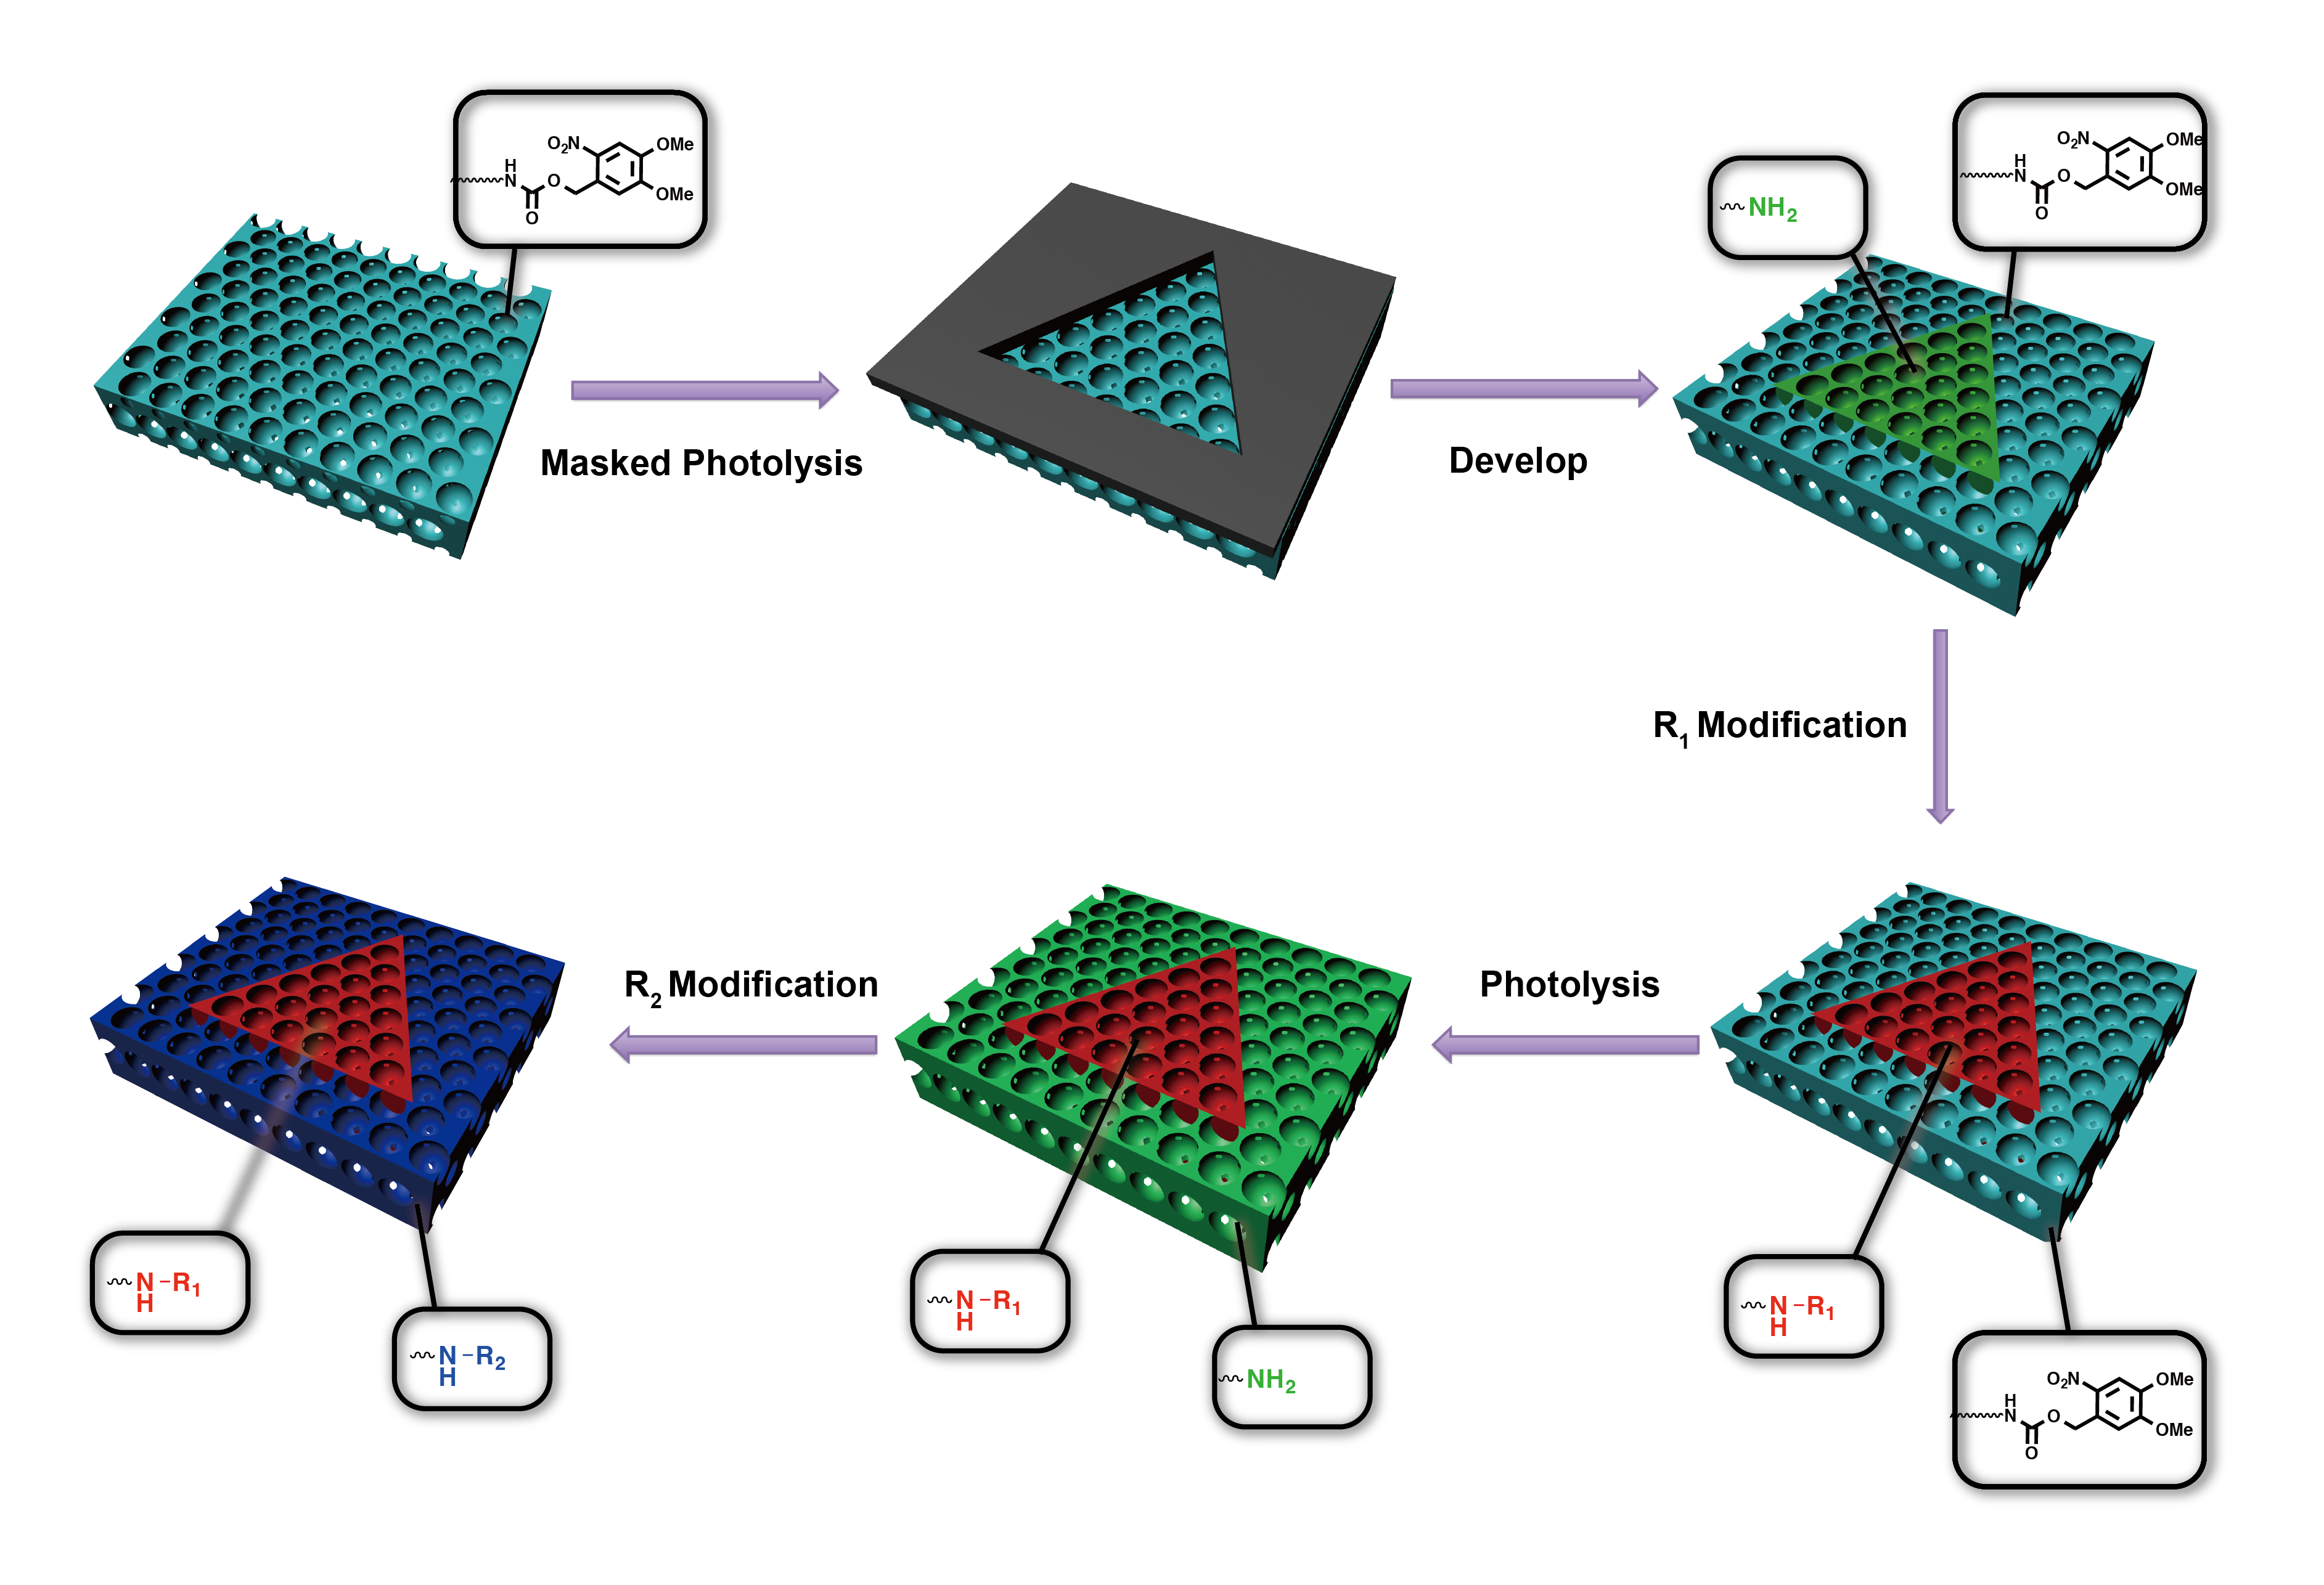
\includegraphics[width=0.9\linewidth]{figures/scheme-2D.png}
  \end{figure}
\end{frame}

% wierd jpg not possible to align on png~?!

\begin{frame}
\frametitle{材料表征}
    \centering
    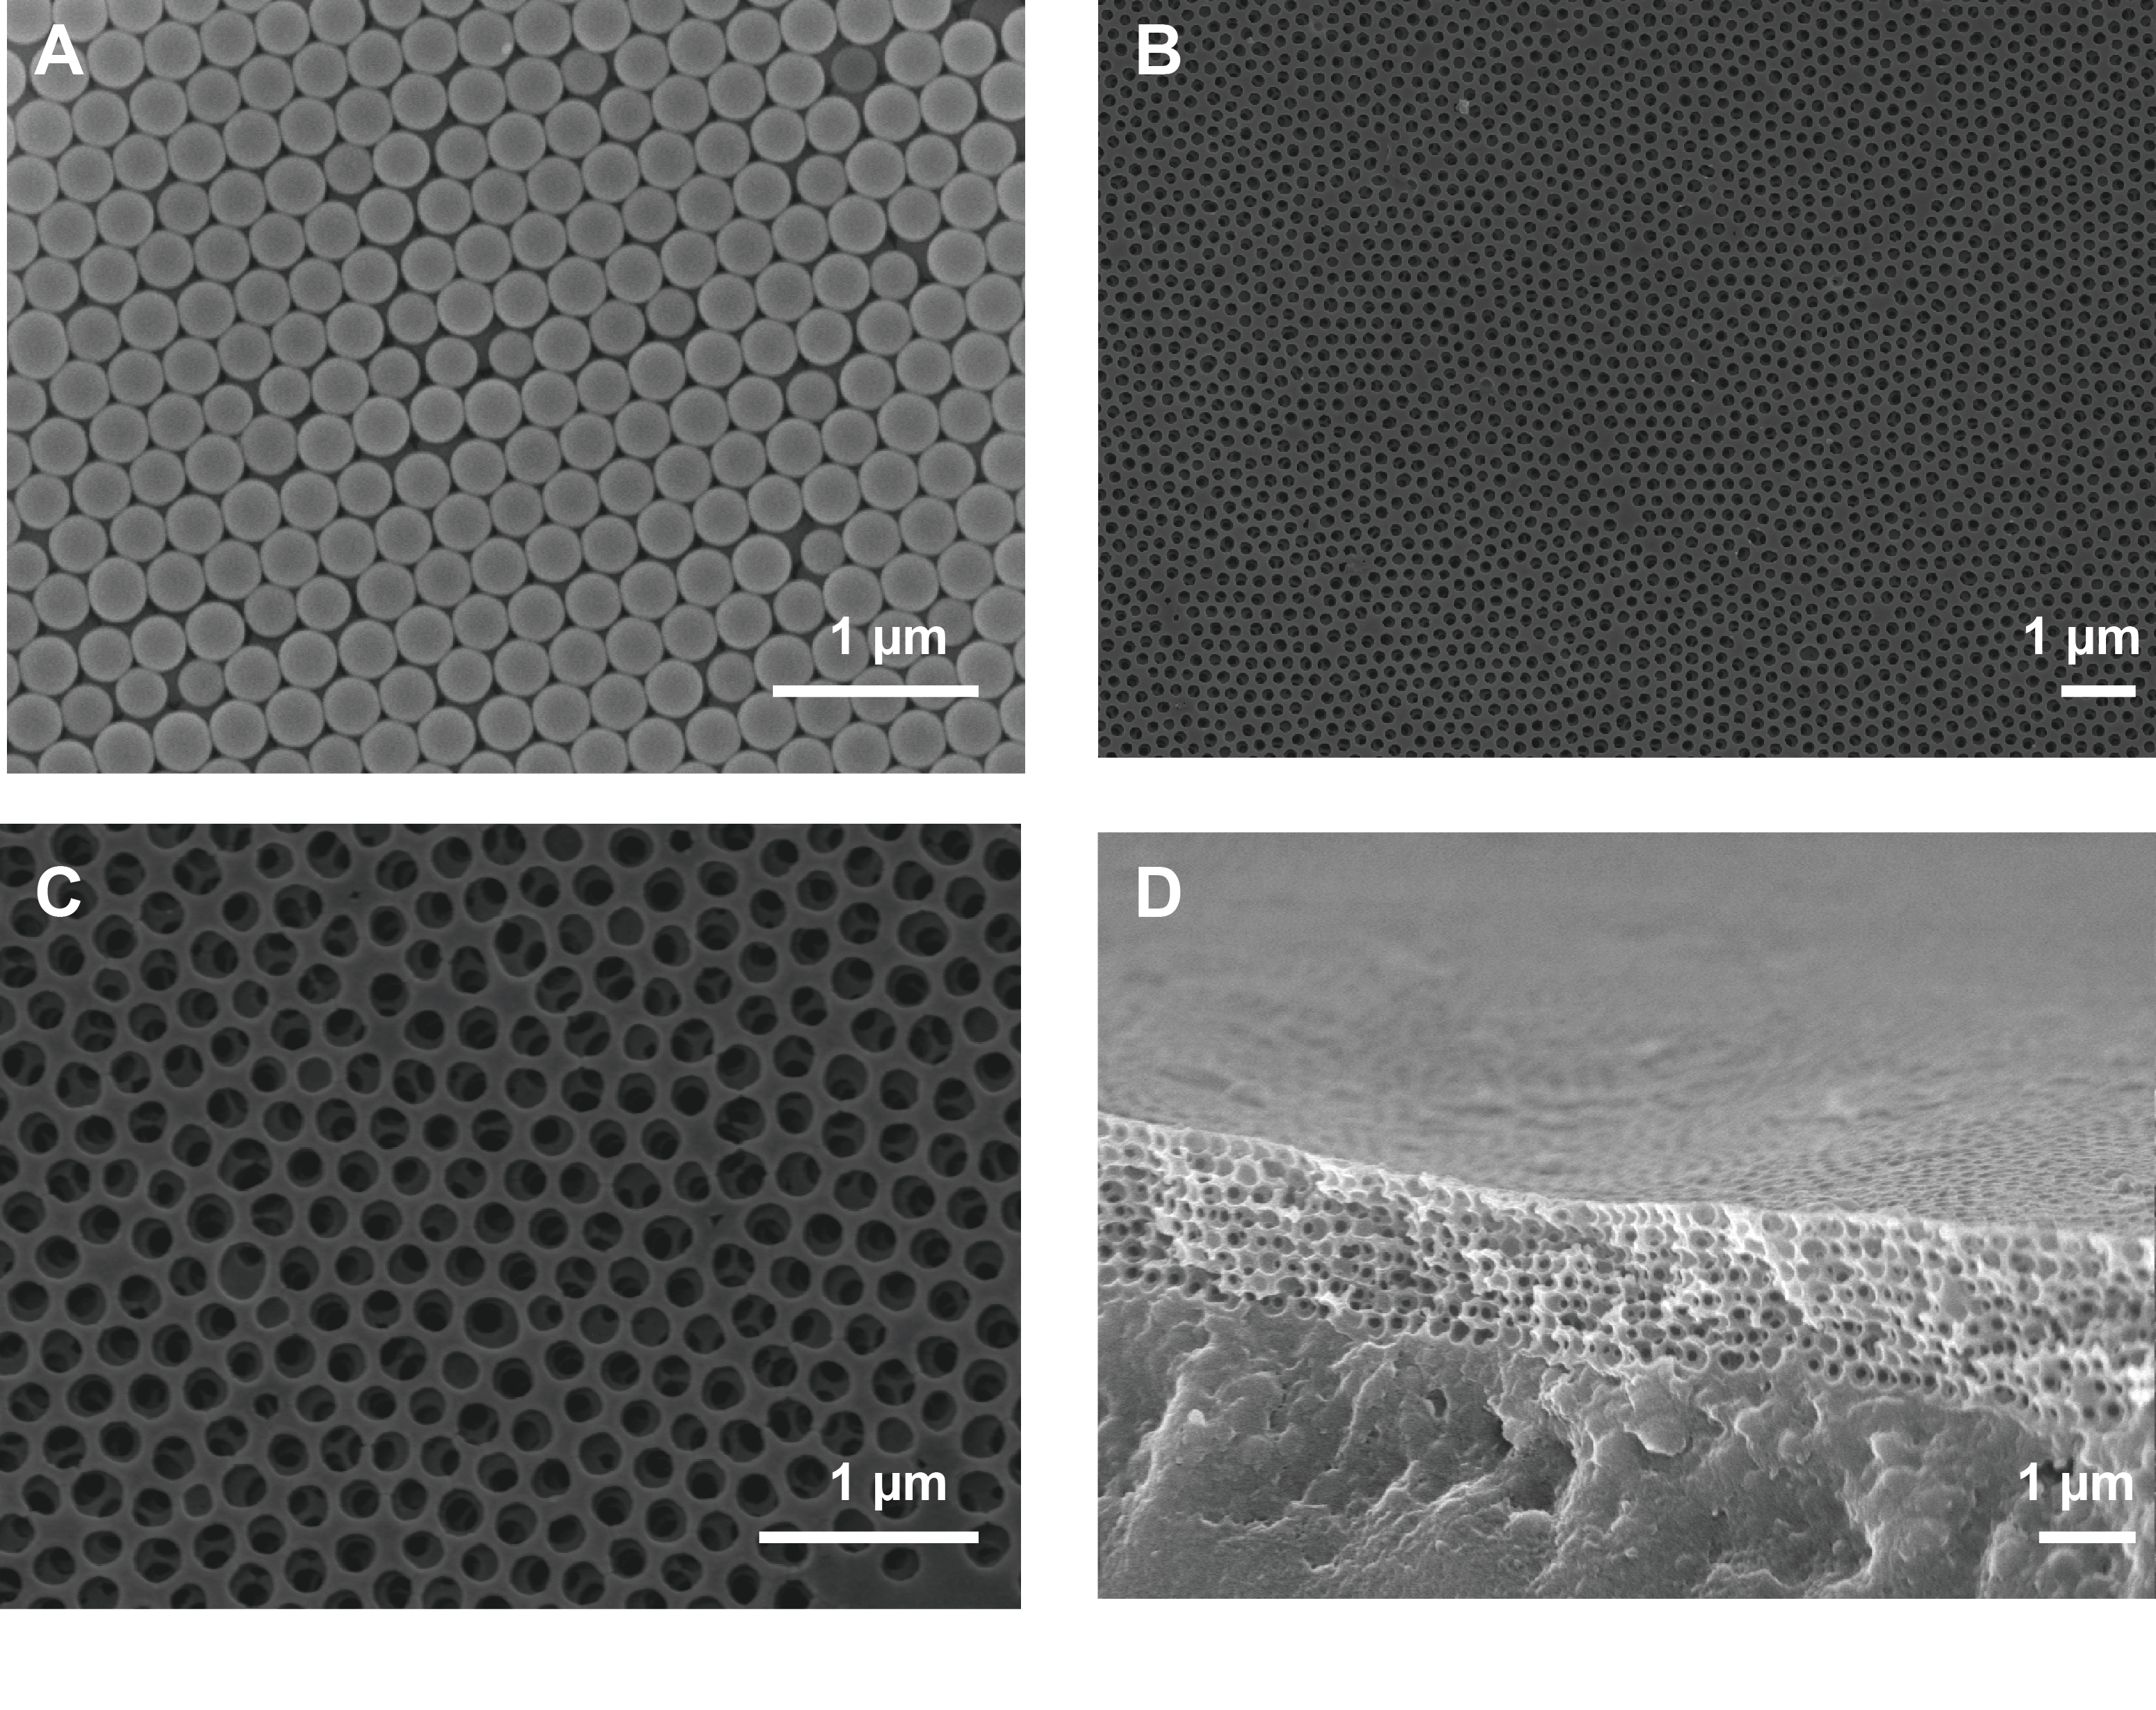
\includegraphics[width=0.85\linewidth]{figures/SEM-ch3.png}
\end{frame}

\begin{frame}
  \frametitle{材料表征}
  \centering
  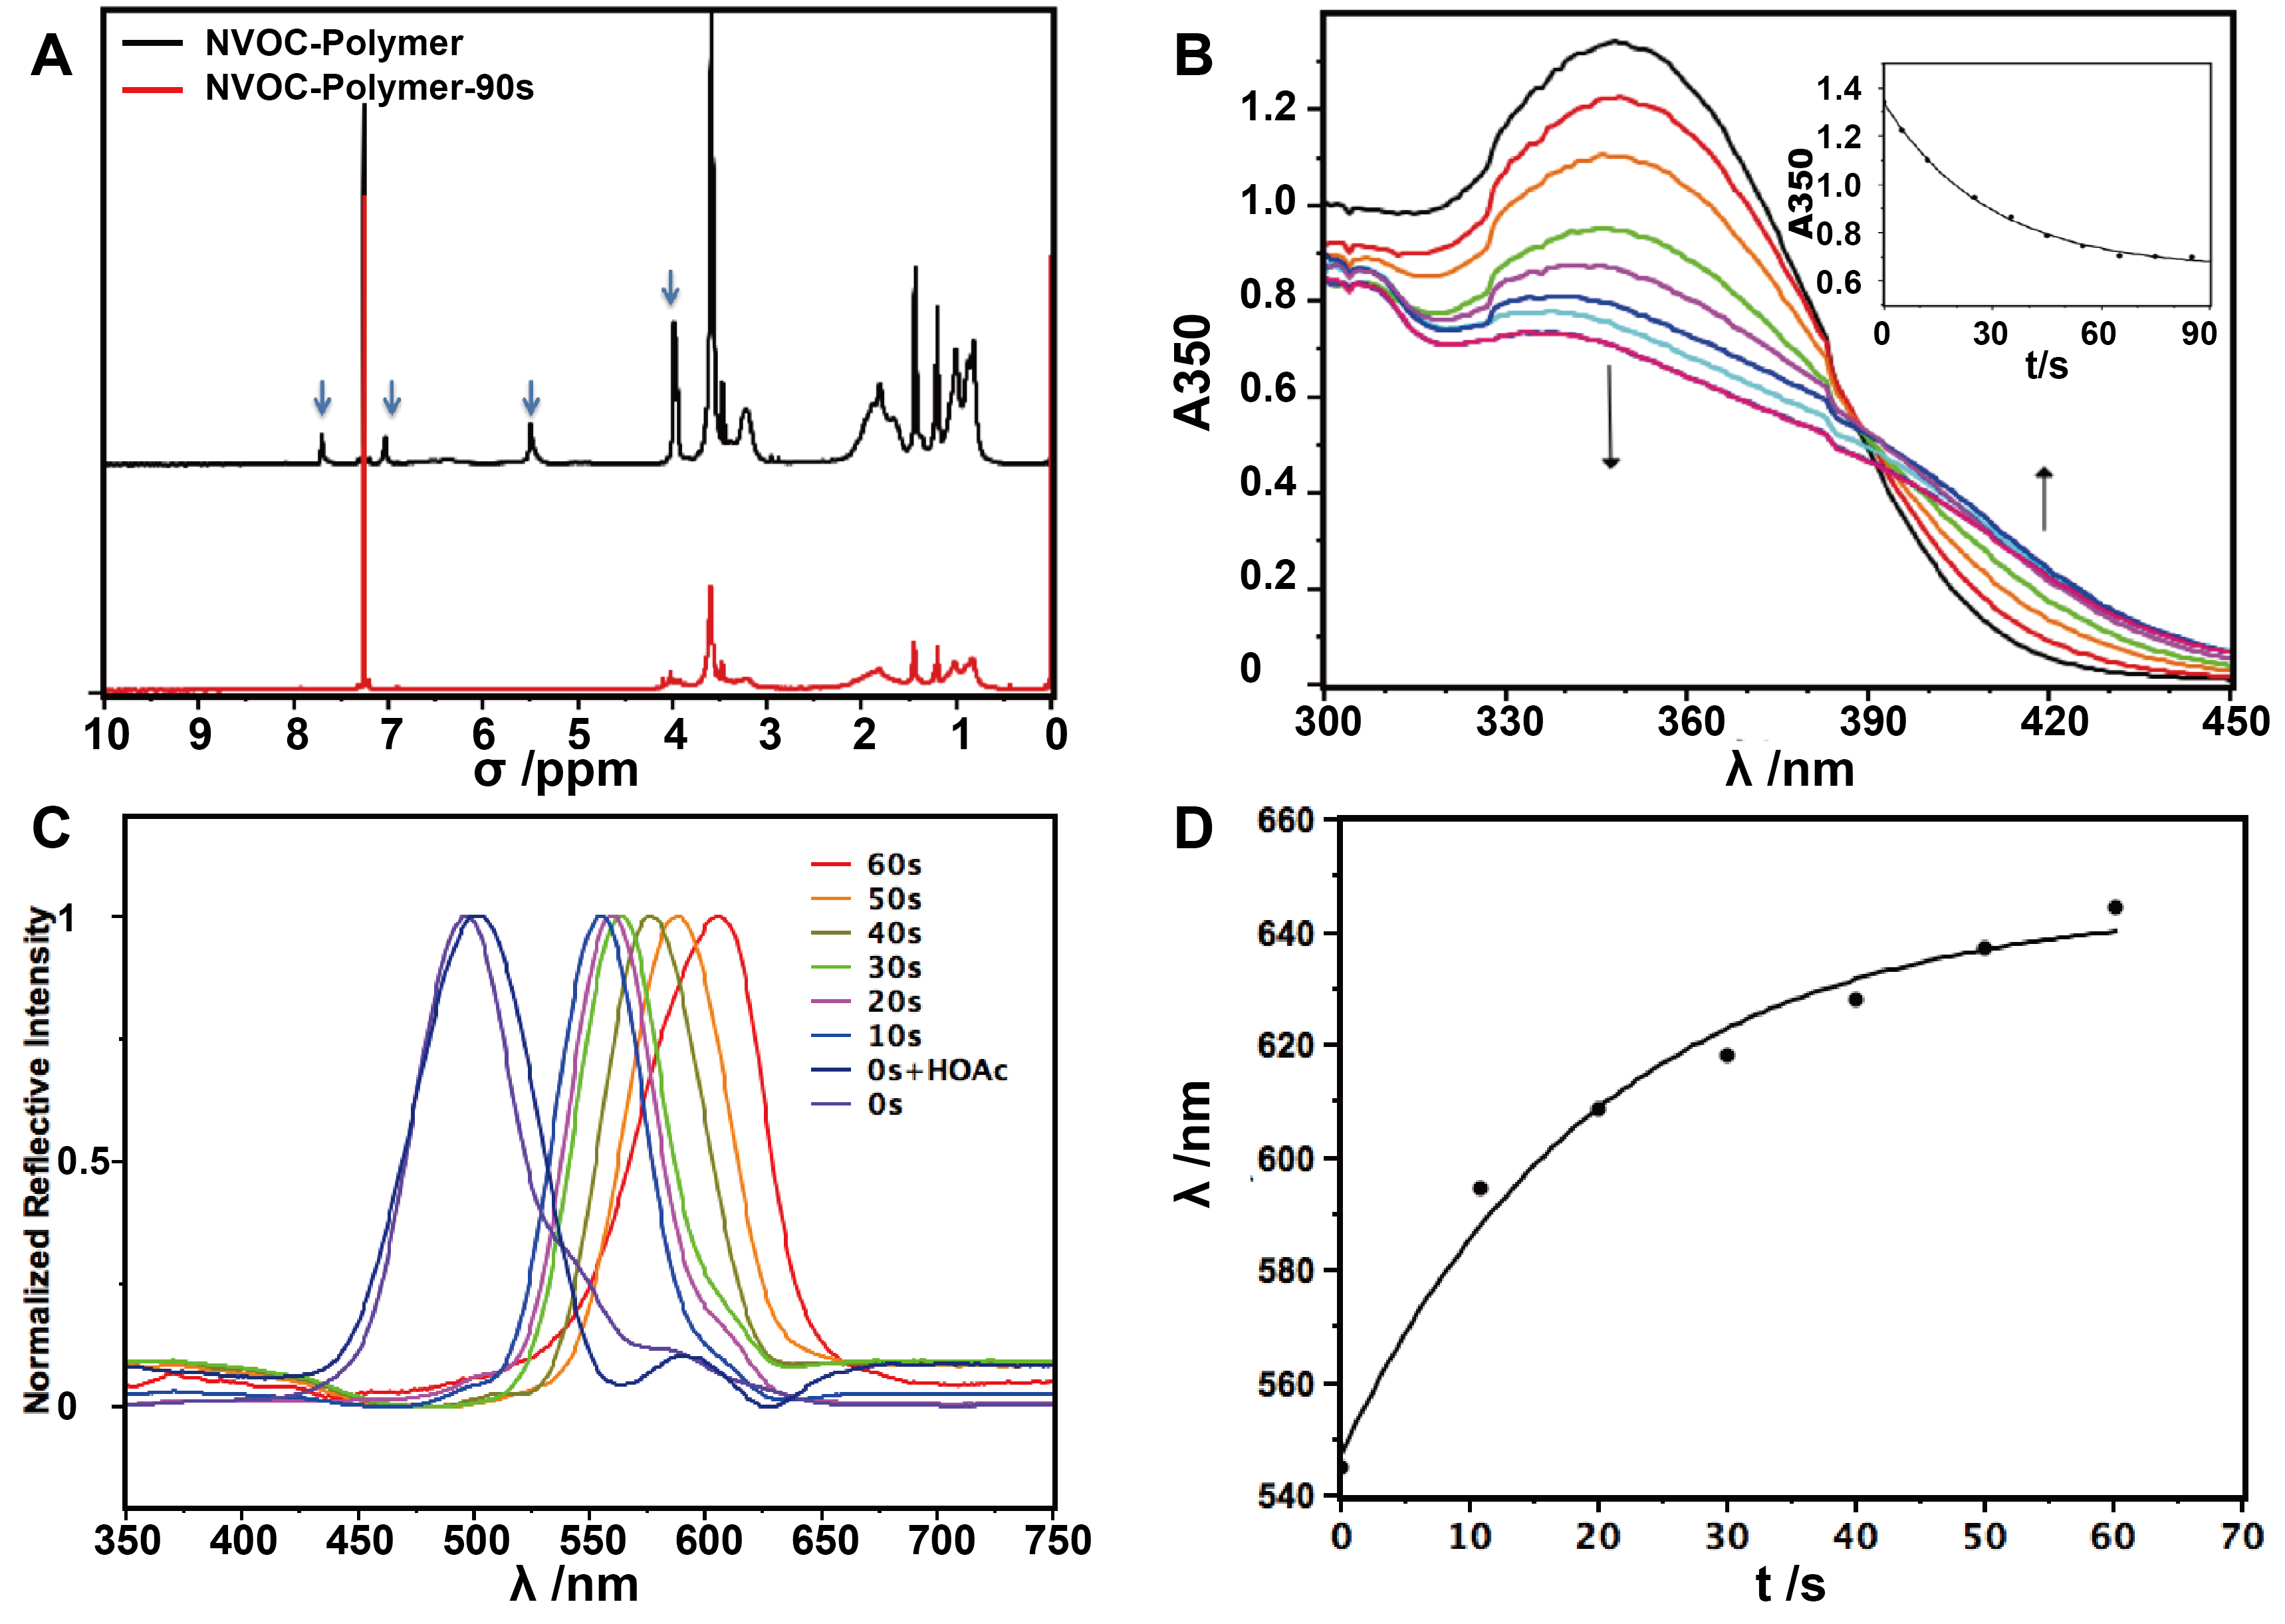
\includegraphics[width=0.9\linewidth]{figures/ch3-characterization.png}
\end{frame}

\begin{frame}
  \frametitle{光子晶体二维亲疏水梯度的实现}
  \begin{minipage}{0.48\textwidth}
  \centering
    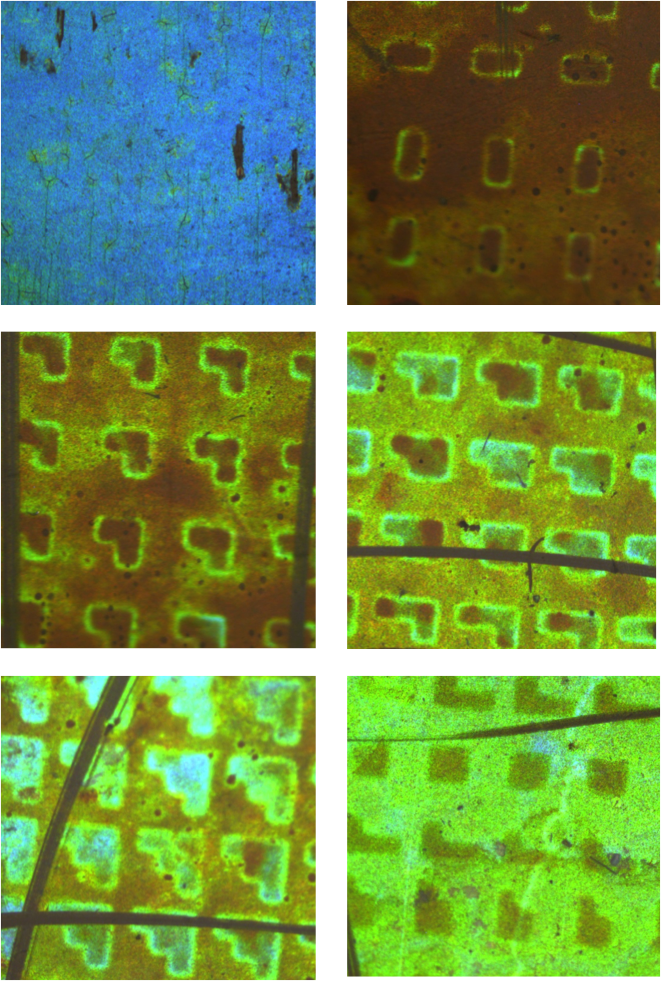
\includegraphics[width=0.85\linewidth]{figures/2D-gradient.png}
  \end{minipage}
  \hfill
  \begin{minipage}{0.48\textwidth}
    \centering
    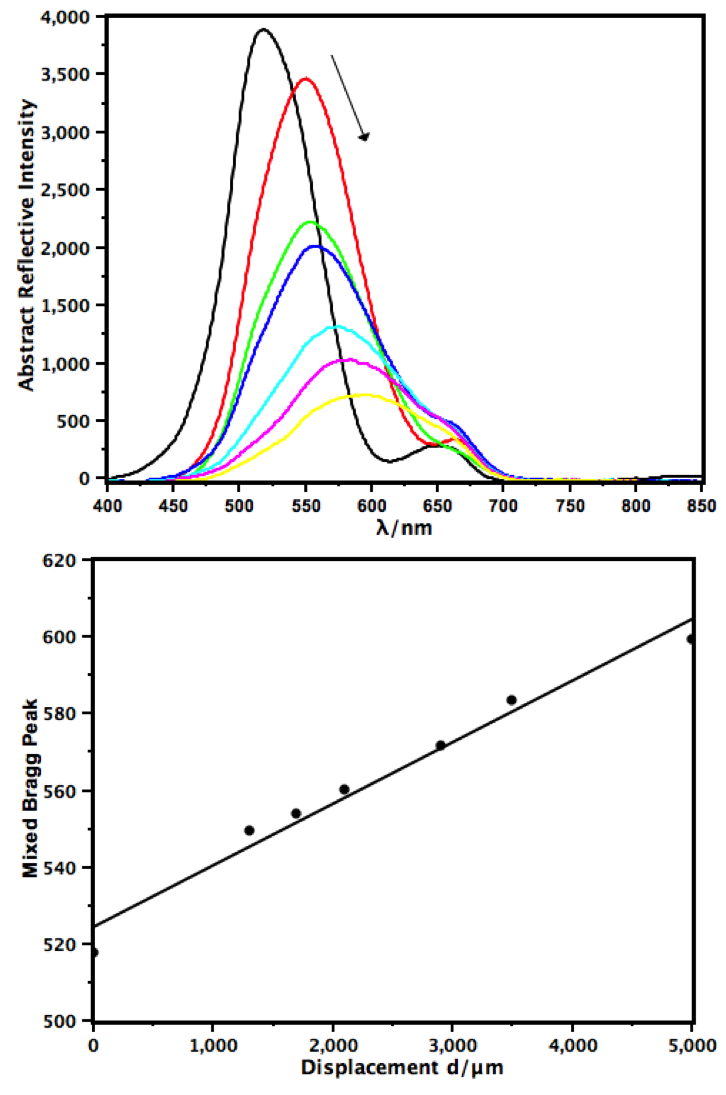
\includegraphics[width=0.85\linewidth]{figures/distance-2D.png}
  \end{minipage}
\end{frame}

% \begin{frame}
%   \frametitle{图案化光子晶体的制备}
%   \begin{figure}
%   \centering
%   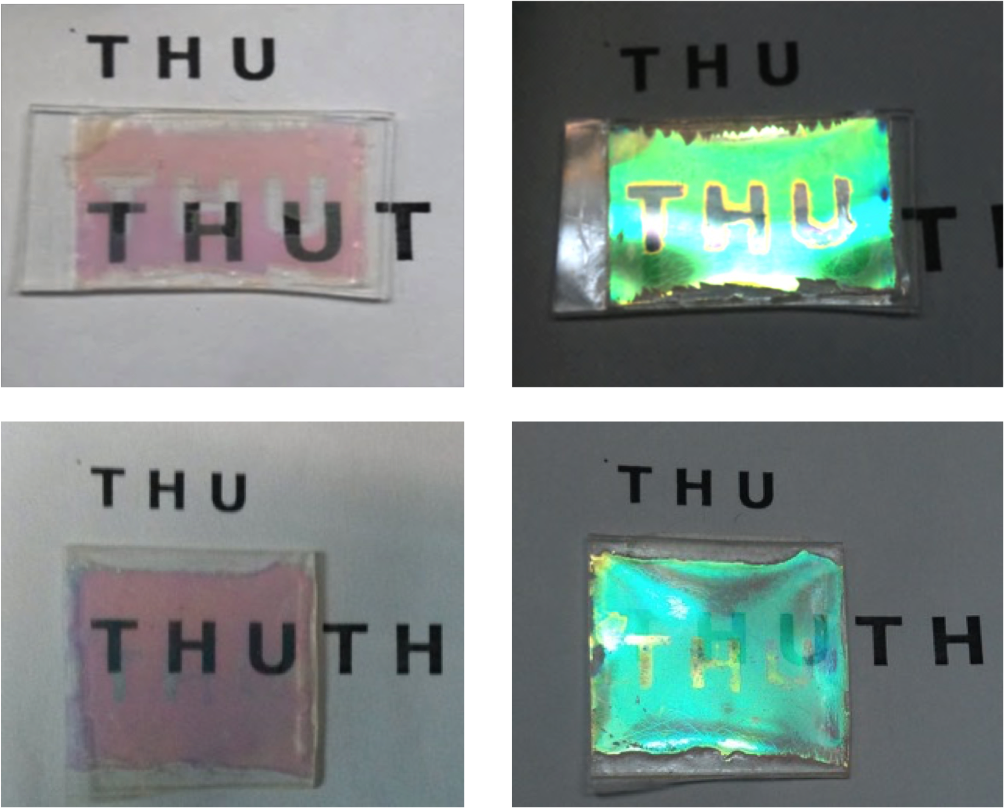
\includegraphics[width=0.76\linewidth]{figures/pattern2DPhC.png}
%   \end{figure}
% \end{frame}

\begin{frame}
  \frametitle{响应性图案化光子晶体}
  \begin{figure}
  \centering
  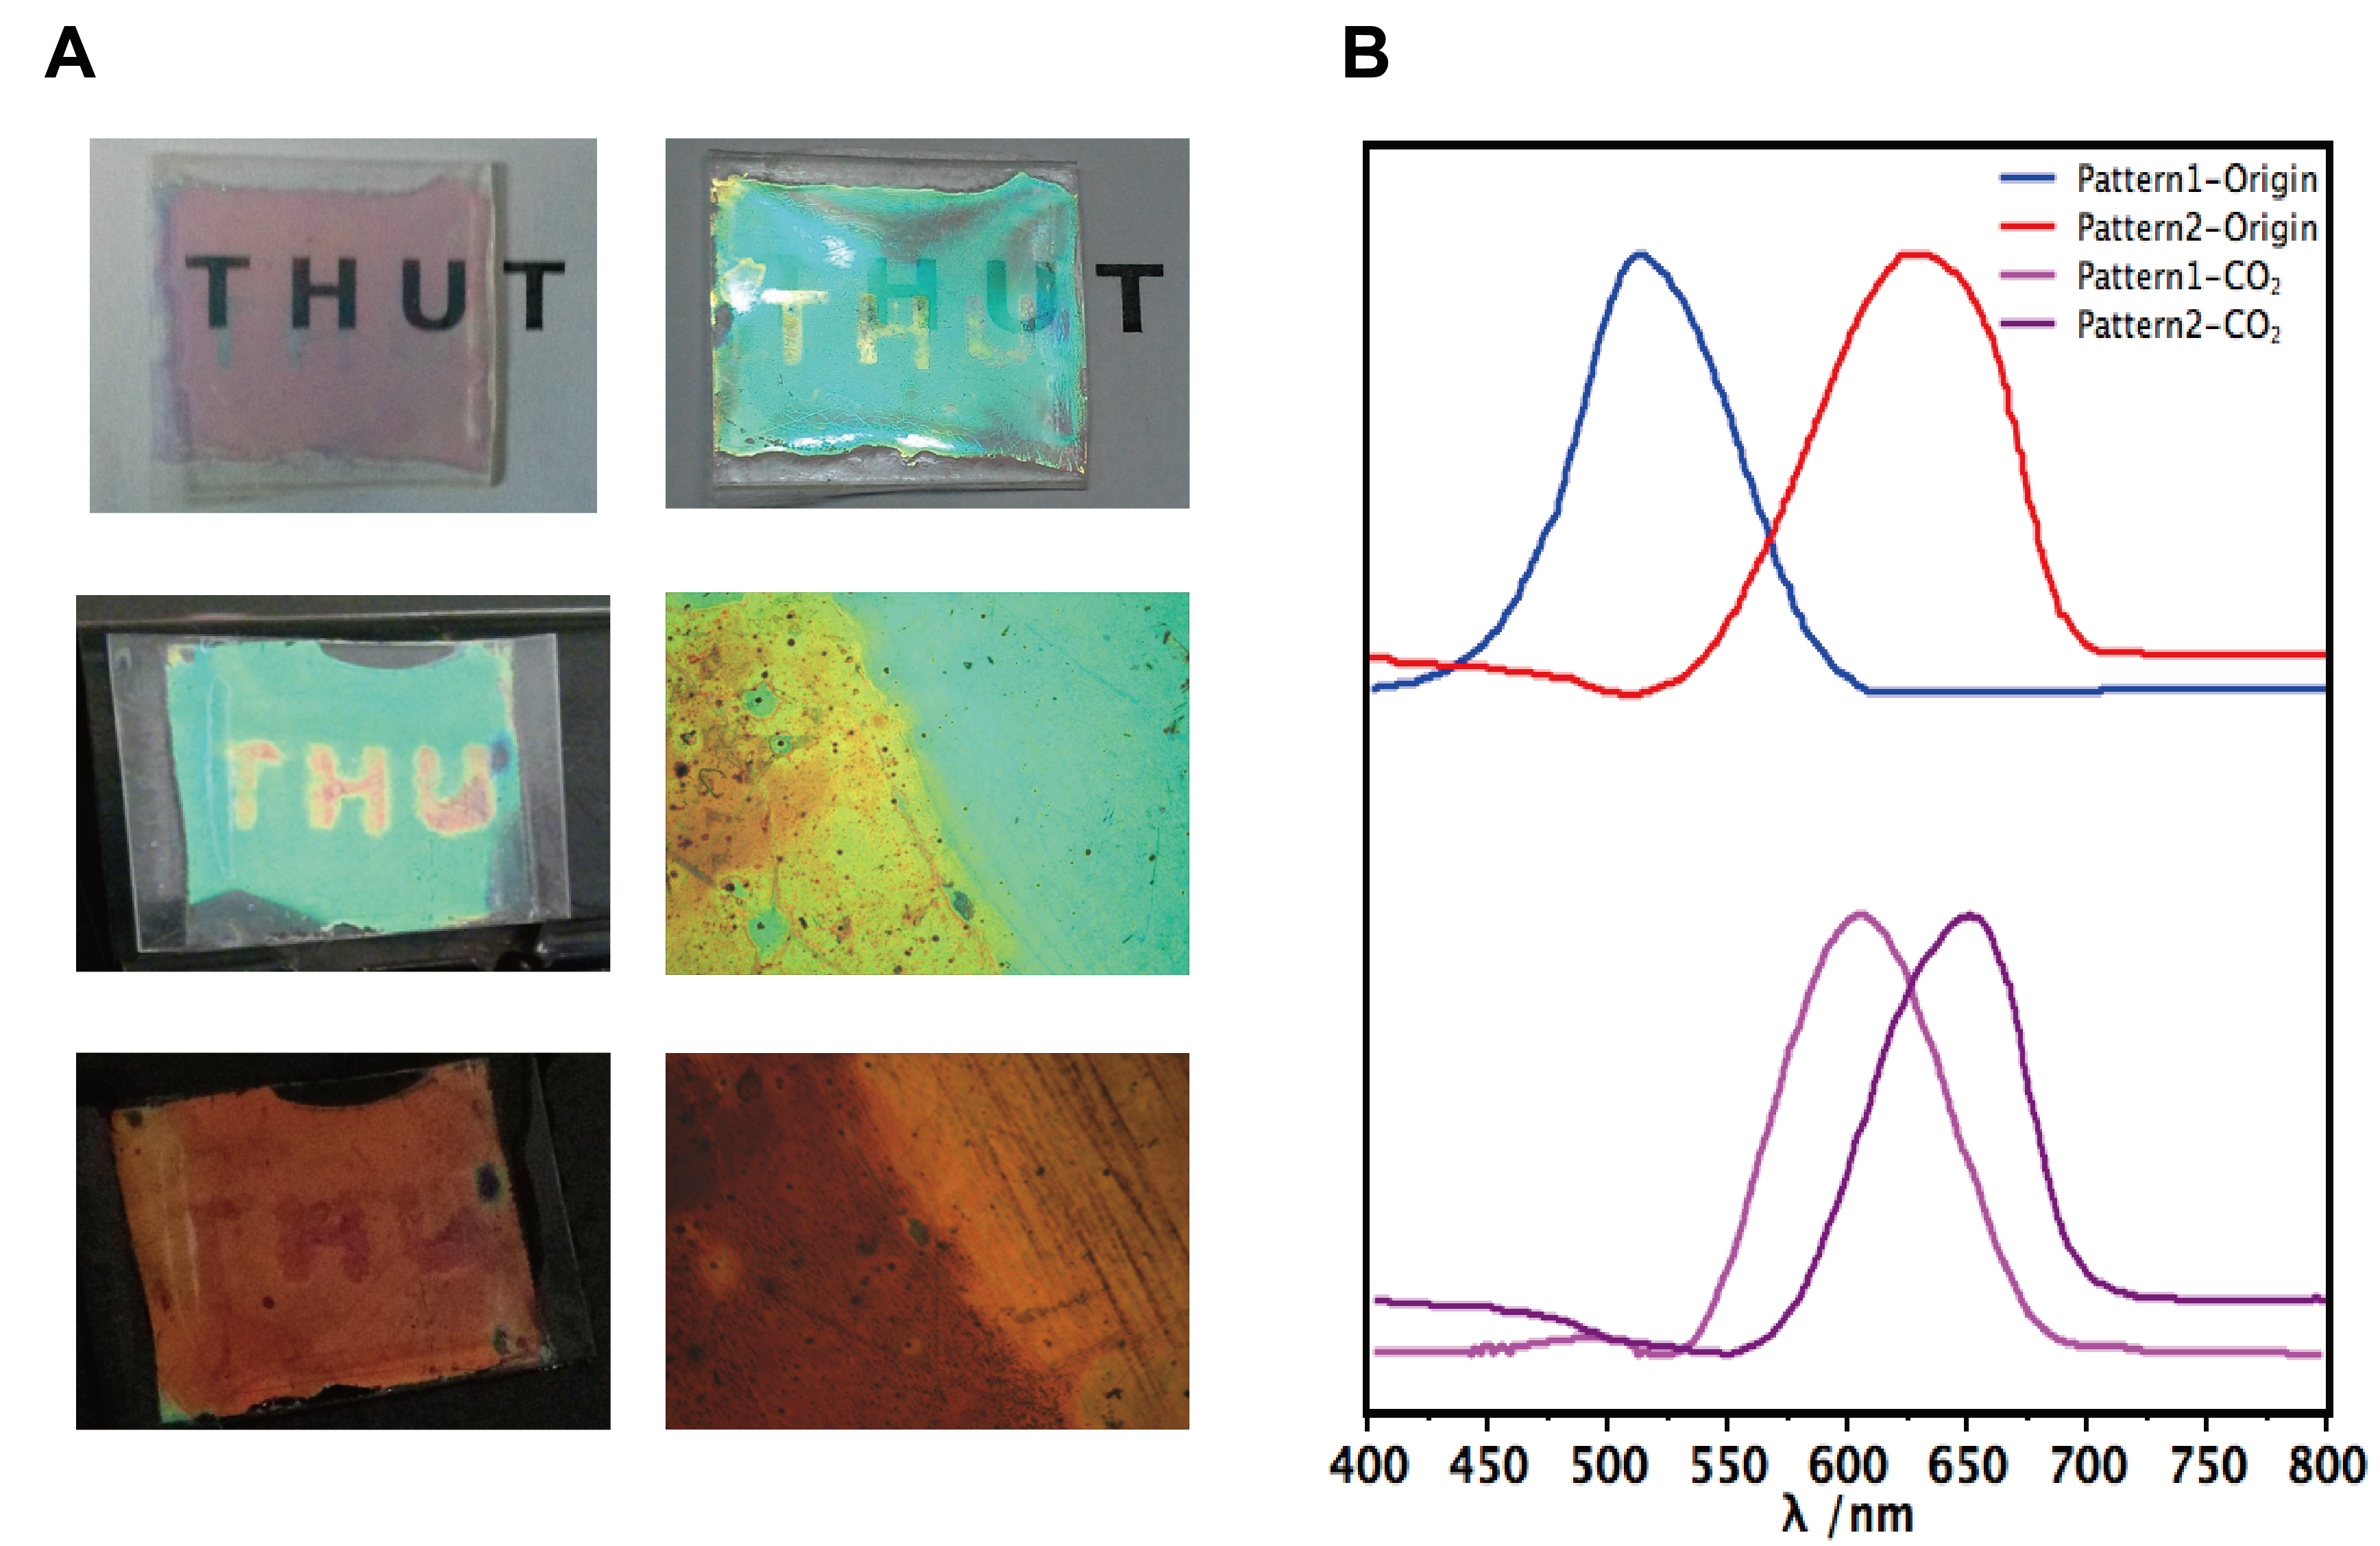
\includegraphics[width=0.95\linewidth]{figures/pattern-dynamic.png}
  \end{figure}
\end{frame}

\begin{frame}
  \frametitle{图案化光子晶体的响应}
  \begin{figure}
  \centering
  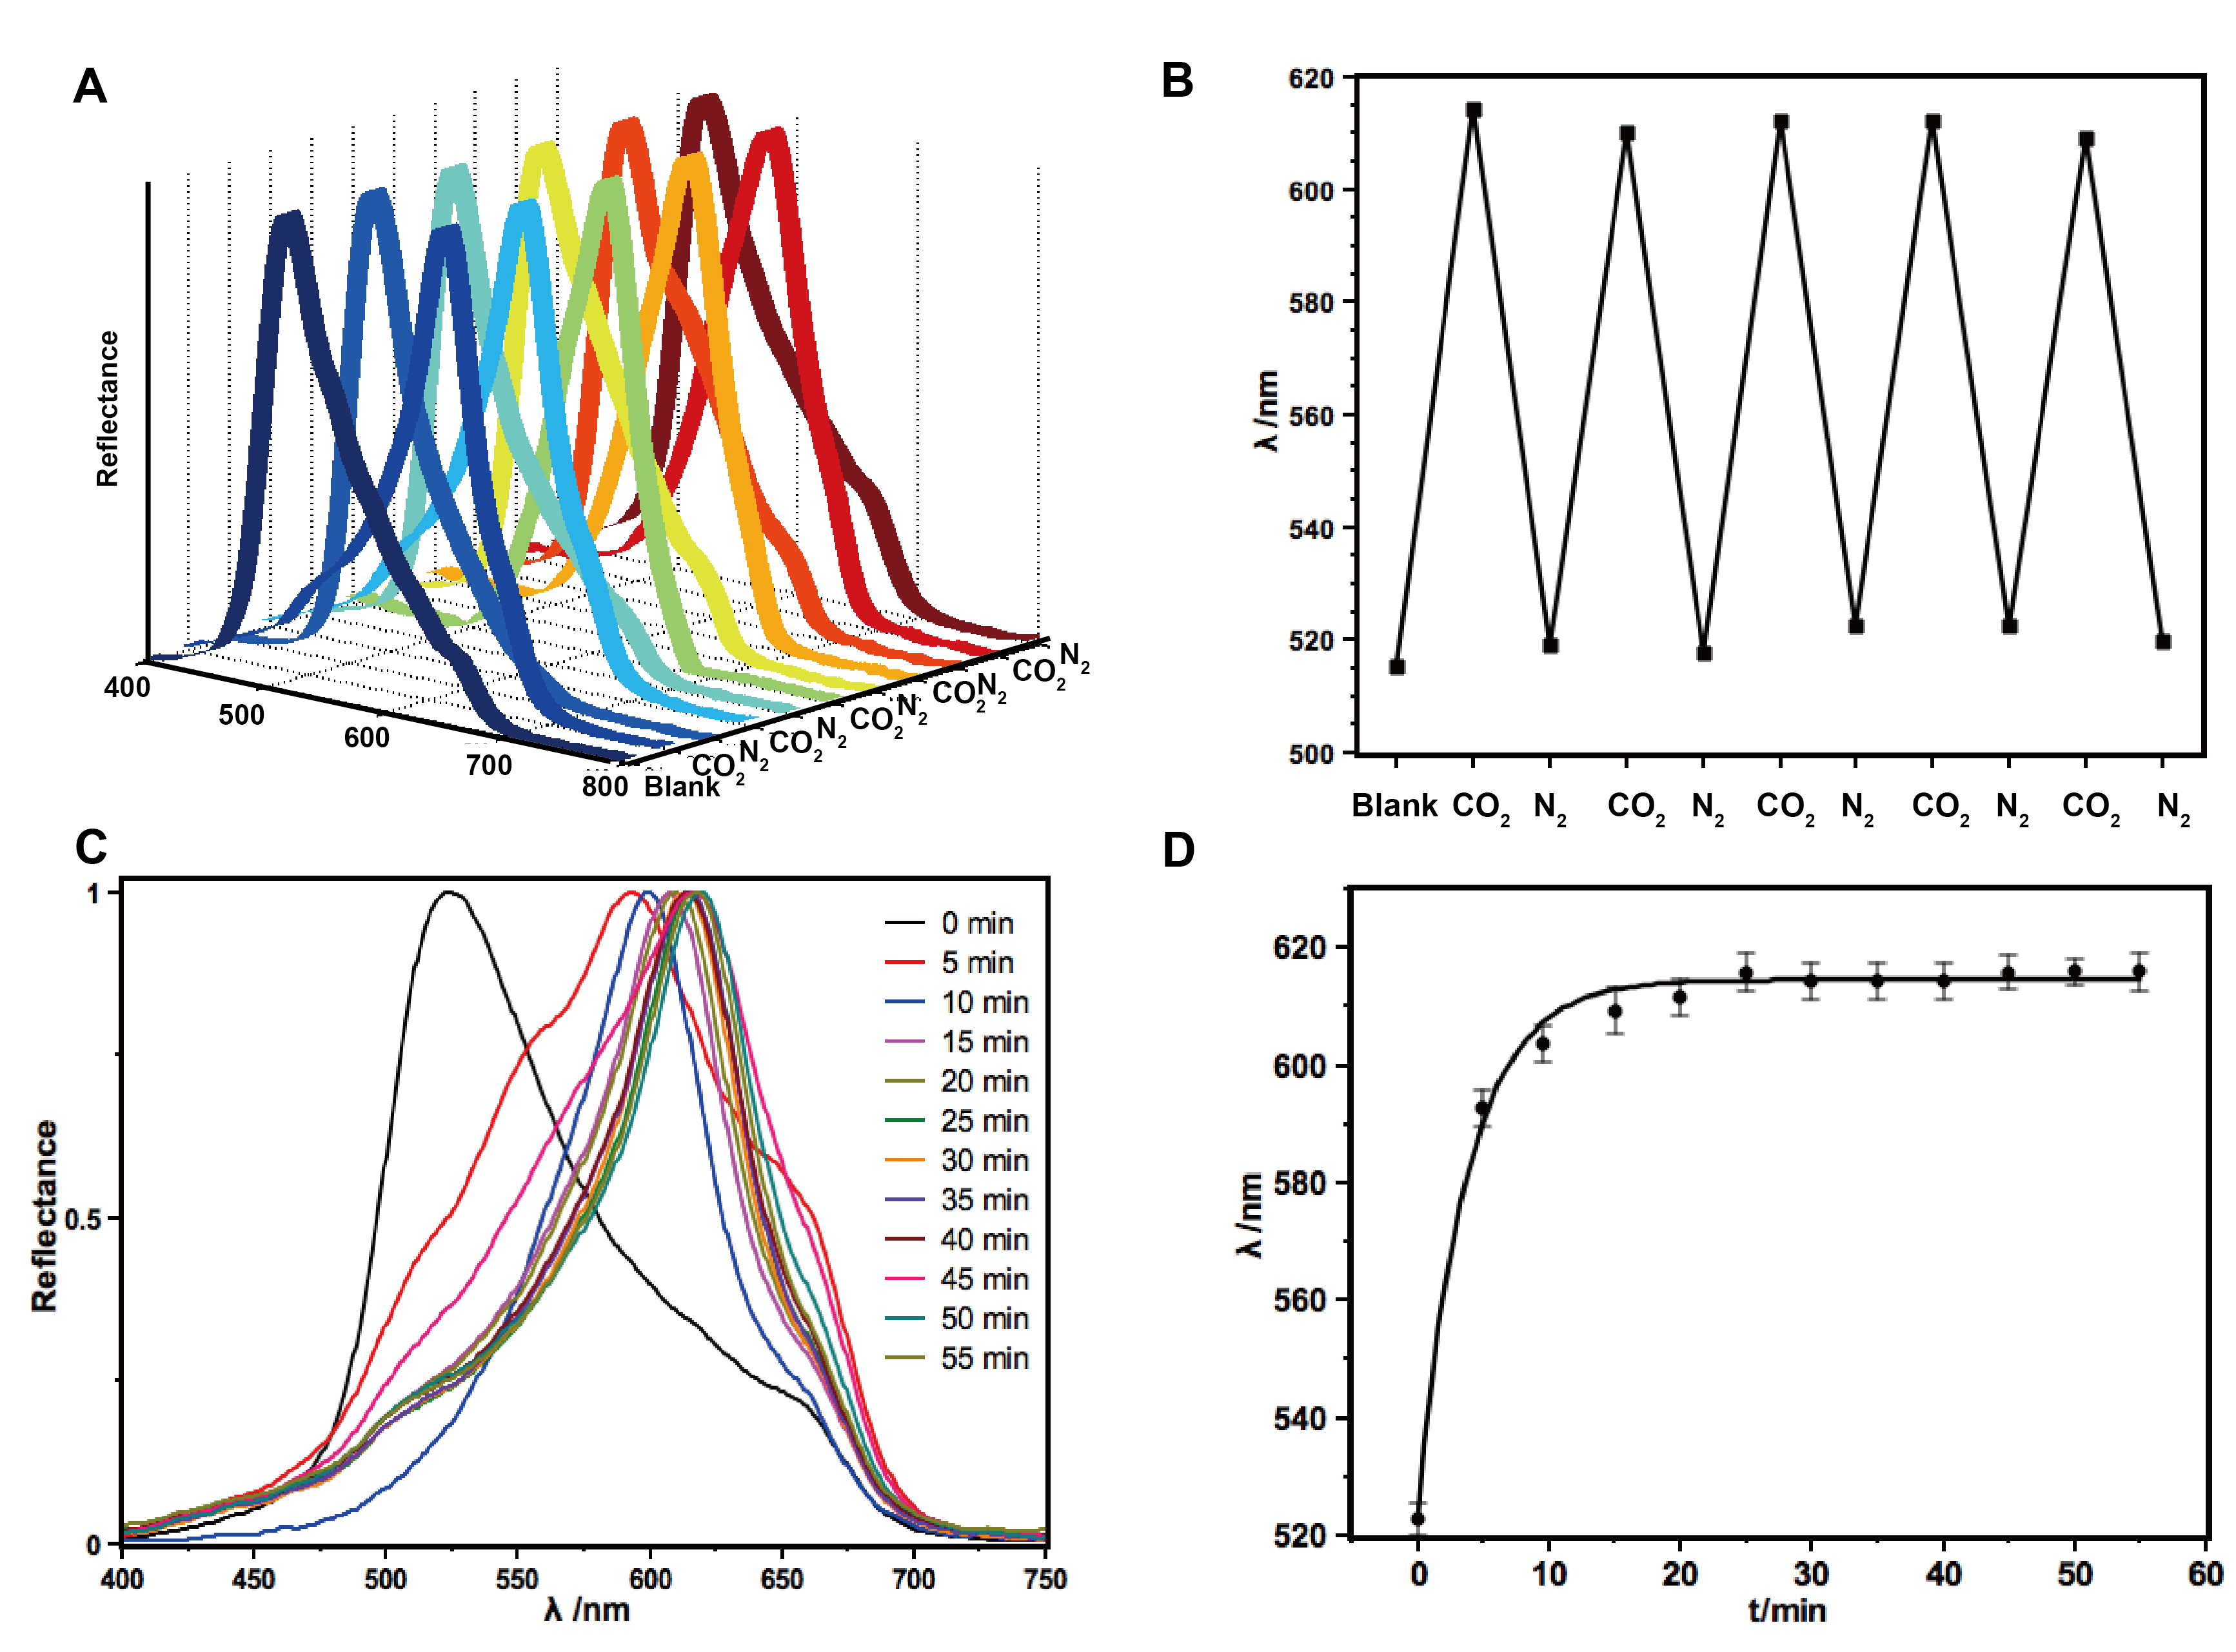
\includegraphics[width=0.85\linewidth]{figures/ch3-saturation.png}
  \end{figure}
\end{frame}

\begin{frame}
  \frametitle{本章小结}
  \begin{itemize}
    \item
    基于光敏高分子实现了平面反蛋白石光子晶体的图案化与复杂化学组成修饰;
    \item
    光子晶体修饰方法简便,通过反应后修饰赋予了光子晶体很大的拓展性;
    \item
    基于选择性光反应-修饰法制备了光子晶体亲疏水梯度图案
    \item
    基于选择性光反应-修饰法制备动态调节的图案化光子晶体
  \end{itemize}
\end{frame}

\subsection{基于刻蚀-反应的光子晶体微球复杂功能体系的研究}

\begin{frame}
  \frametitle{图案化/复杂功能化:2D->3D?}
  \textcolor{tsinghua}{\textbf{光子晶体三维功能化的难点与潜力}}
  \begin{itemize}
    \item
    选择性光反应-修饰只适用于平面型光子晶体材料;
    \item
    空间上的复杂化学/光学性质具有很大潜在研究与应用价值;
    \item
    光子晶体光学特性、孔道结构、复杂化学组成协同作用体系。
  \end{itemize}
  \pause
  \textcolor{tsinghua}{\textbf{可能的解决方案:}}
  光子晶体微球+选择性刻蚀-反应
\end{frame}

\begin{frame}
  \frametitle{实验原理}
  \begin{figure}[htbp]
    \begin{center}
      \includegraphics[width=0.87\linewidth]{figures/ch3/etch-react-3D.png}
    \end{center}
  \end{figure}
\end{frame}

\begin{frame}
  \frametitle{实验原理}
  \begin{figure}
    \begin{center}
      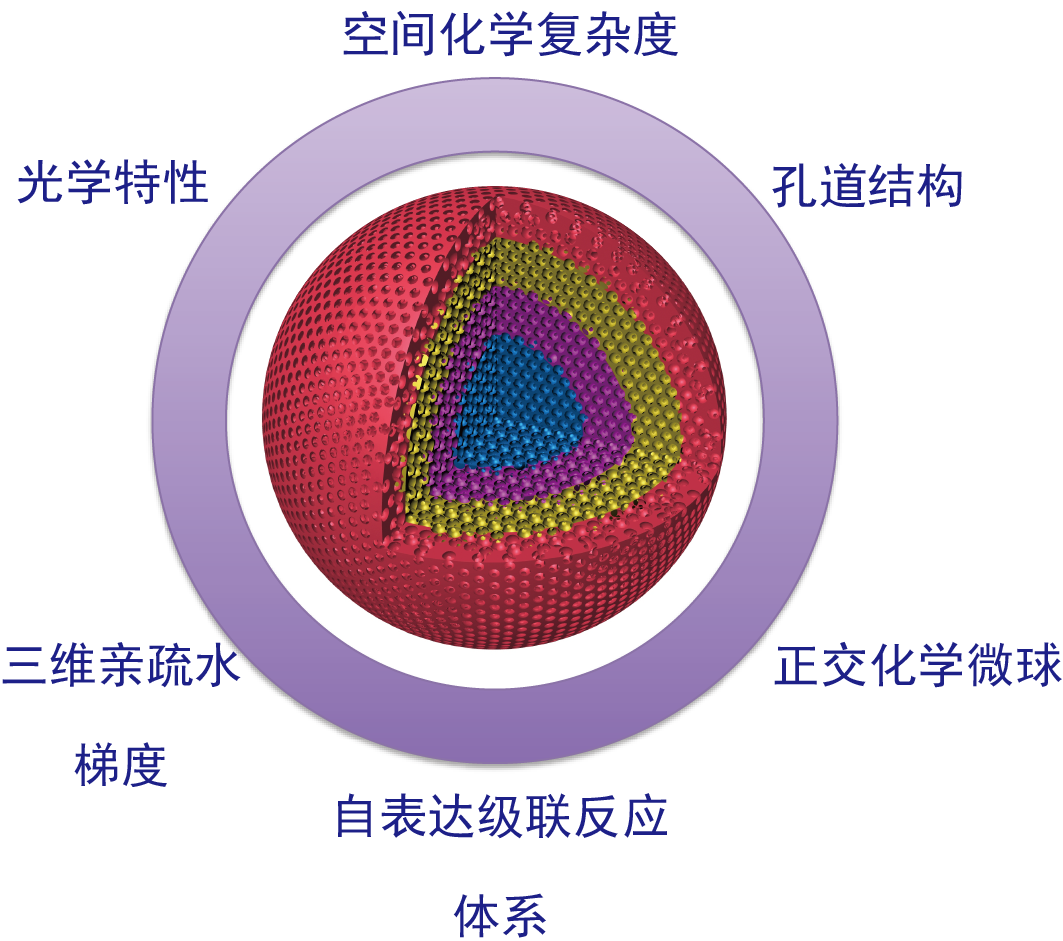
\includegraphics[height=0.65\linewidth]{figures/schem3-2.png}
    \end{center}
  \end{figure}
\end{frame}

% \begin{frame}
%   \frametitle{原理验证}
%   \begin{figure}
%     \begin{center}
%       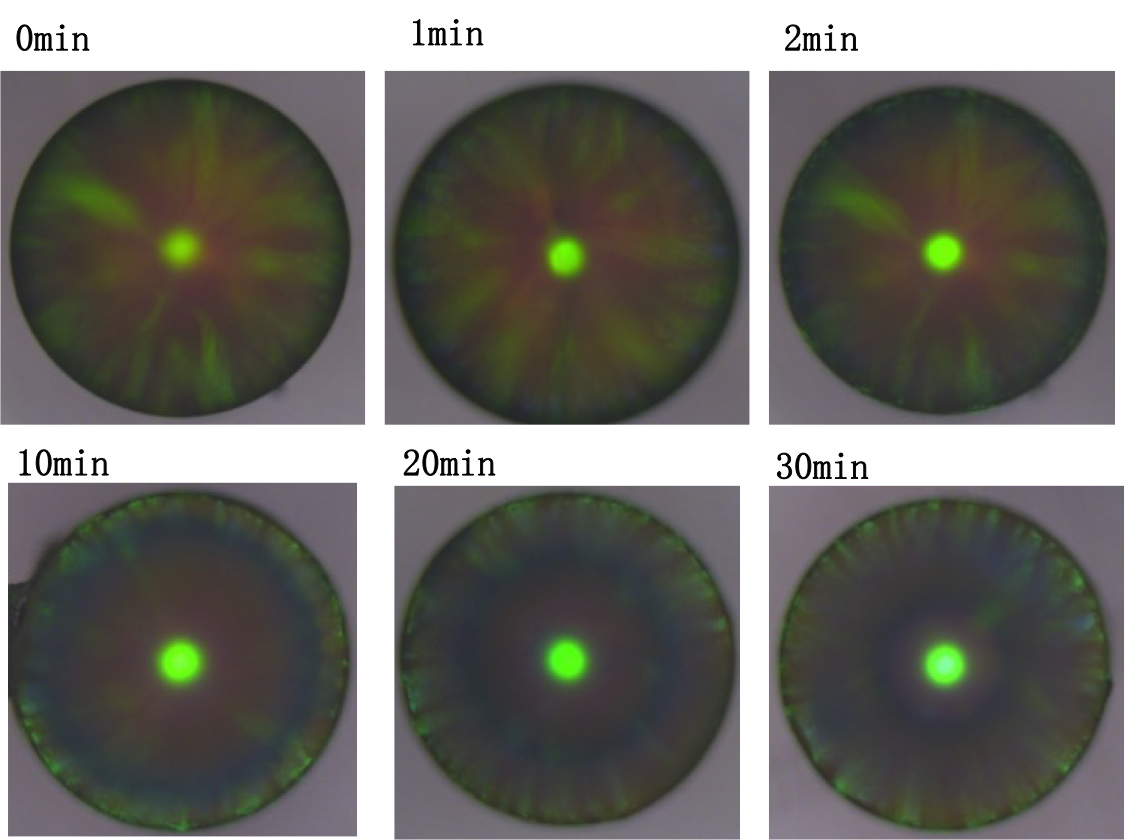
\includegraphics[width=0.8\linewidth]{figures/ch3/Fig1A.png}
%     \end{center}
%   \end{figure}
% \end{frame}

\begin{frame}
  \frametitle{原理验证}
  \begin{figure}
    \begin{center}
      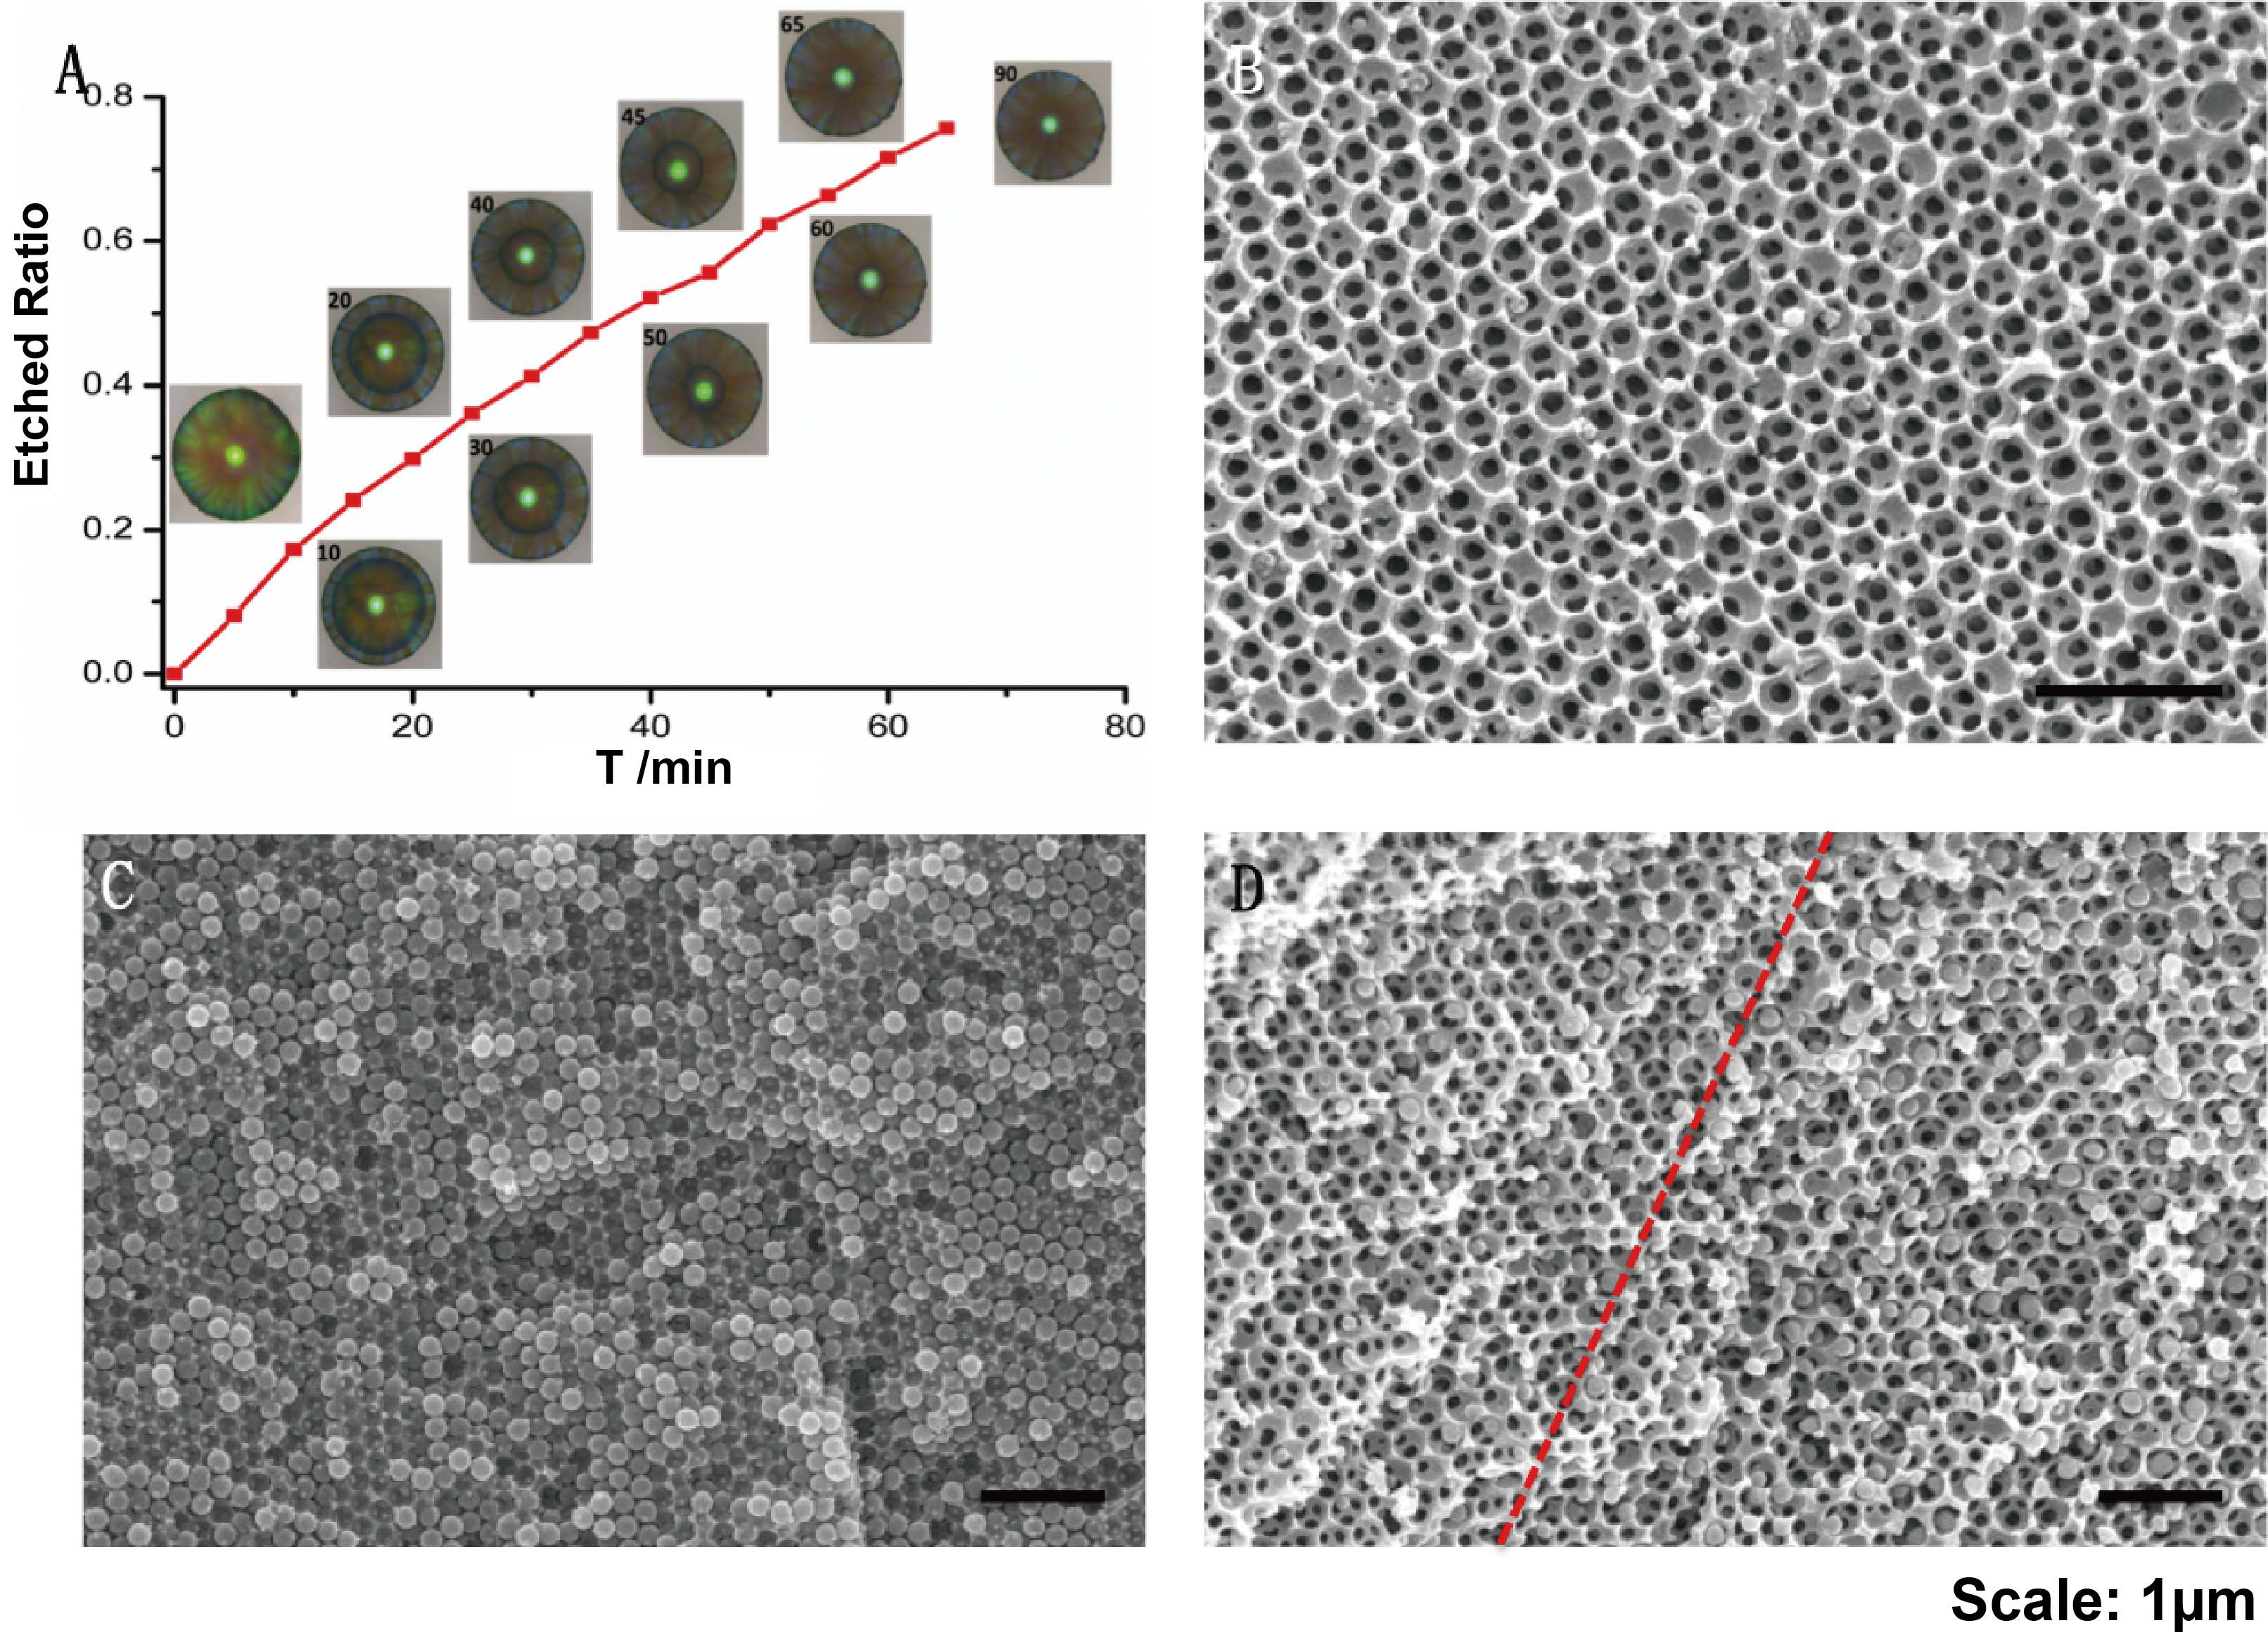
\includegraphics[width=0.85\linewidth]{figures/ch3/Etch-chara.png}
    \end{center}
  \end{figure}
\end{frame}

\begin{frame}
  \frametitle{原理验证}
  \begin{figure}
    \begin{center}
      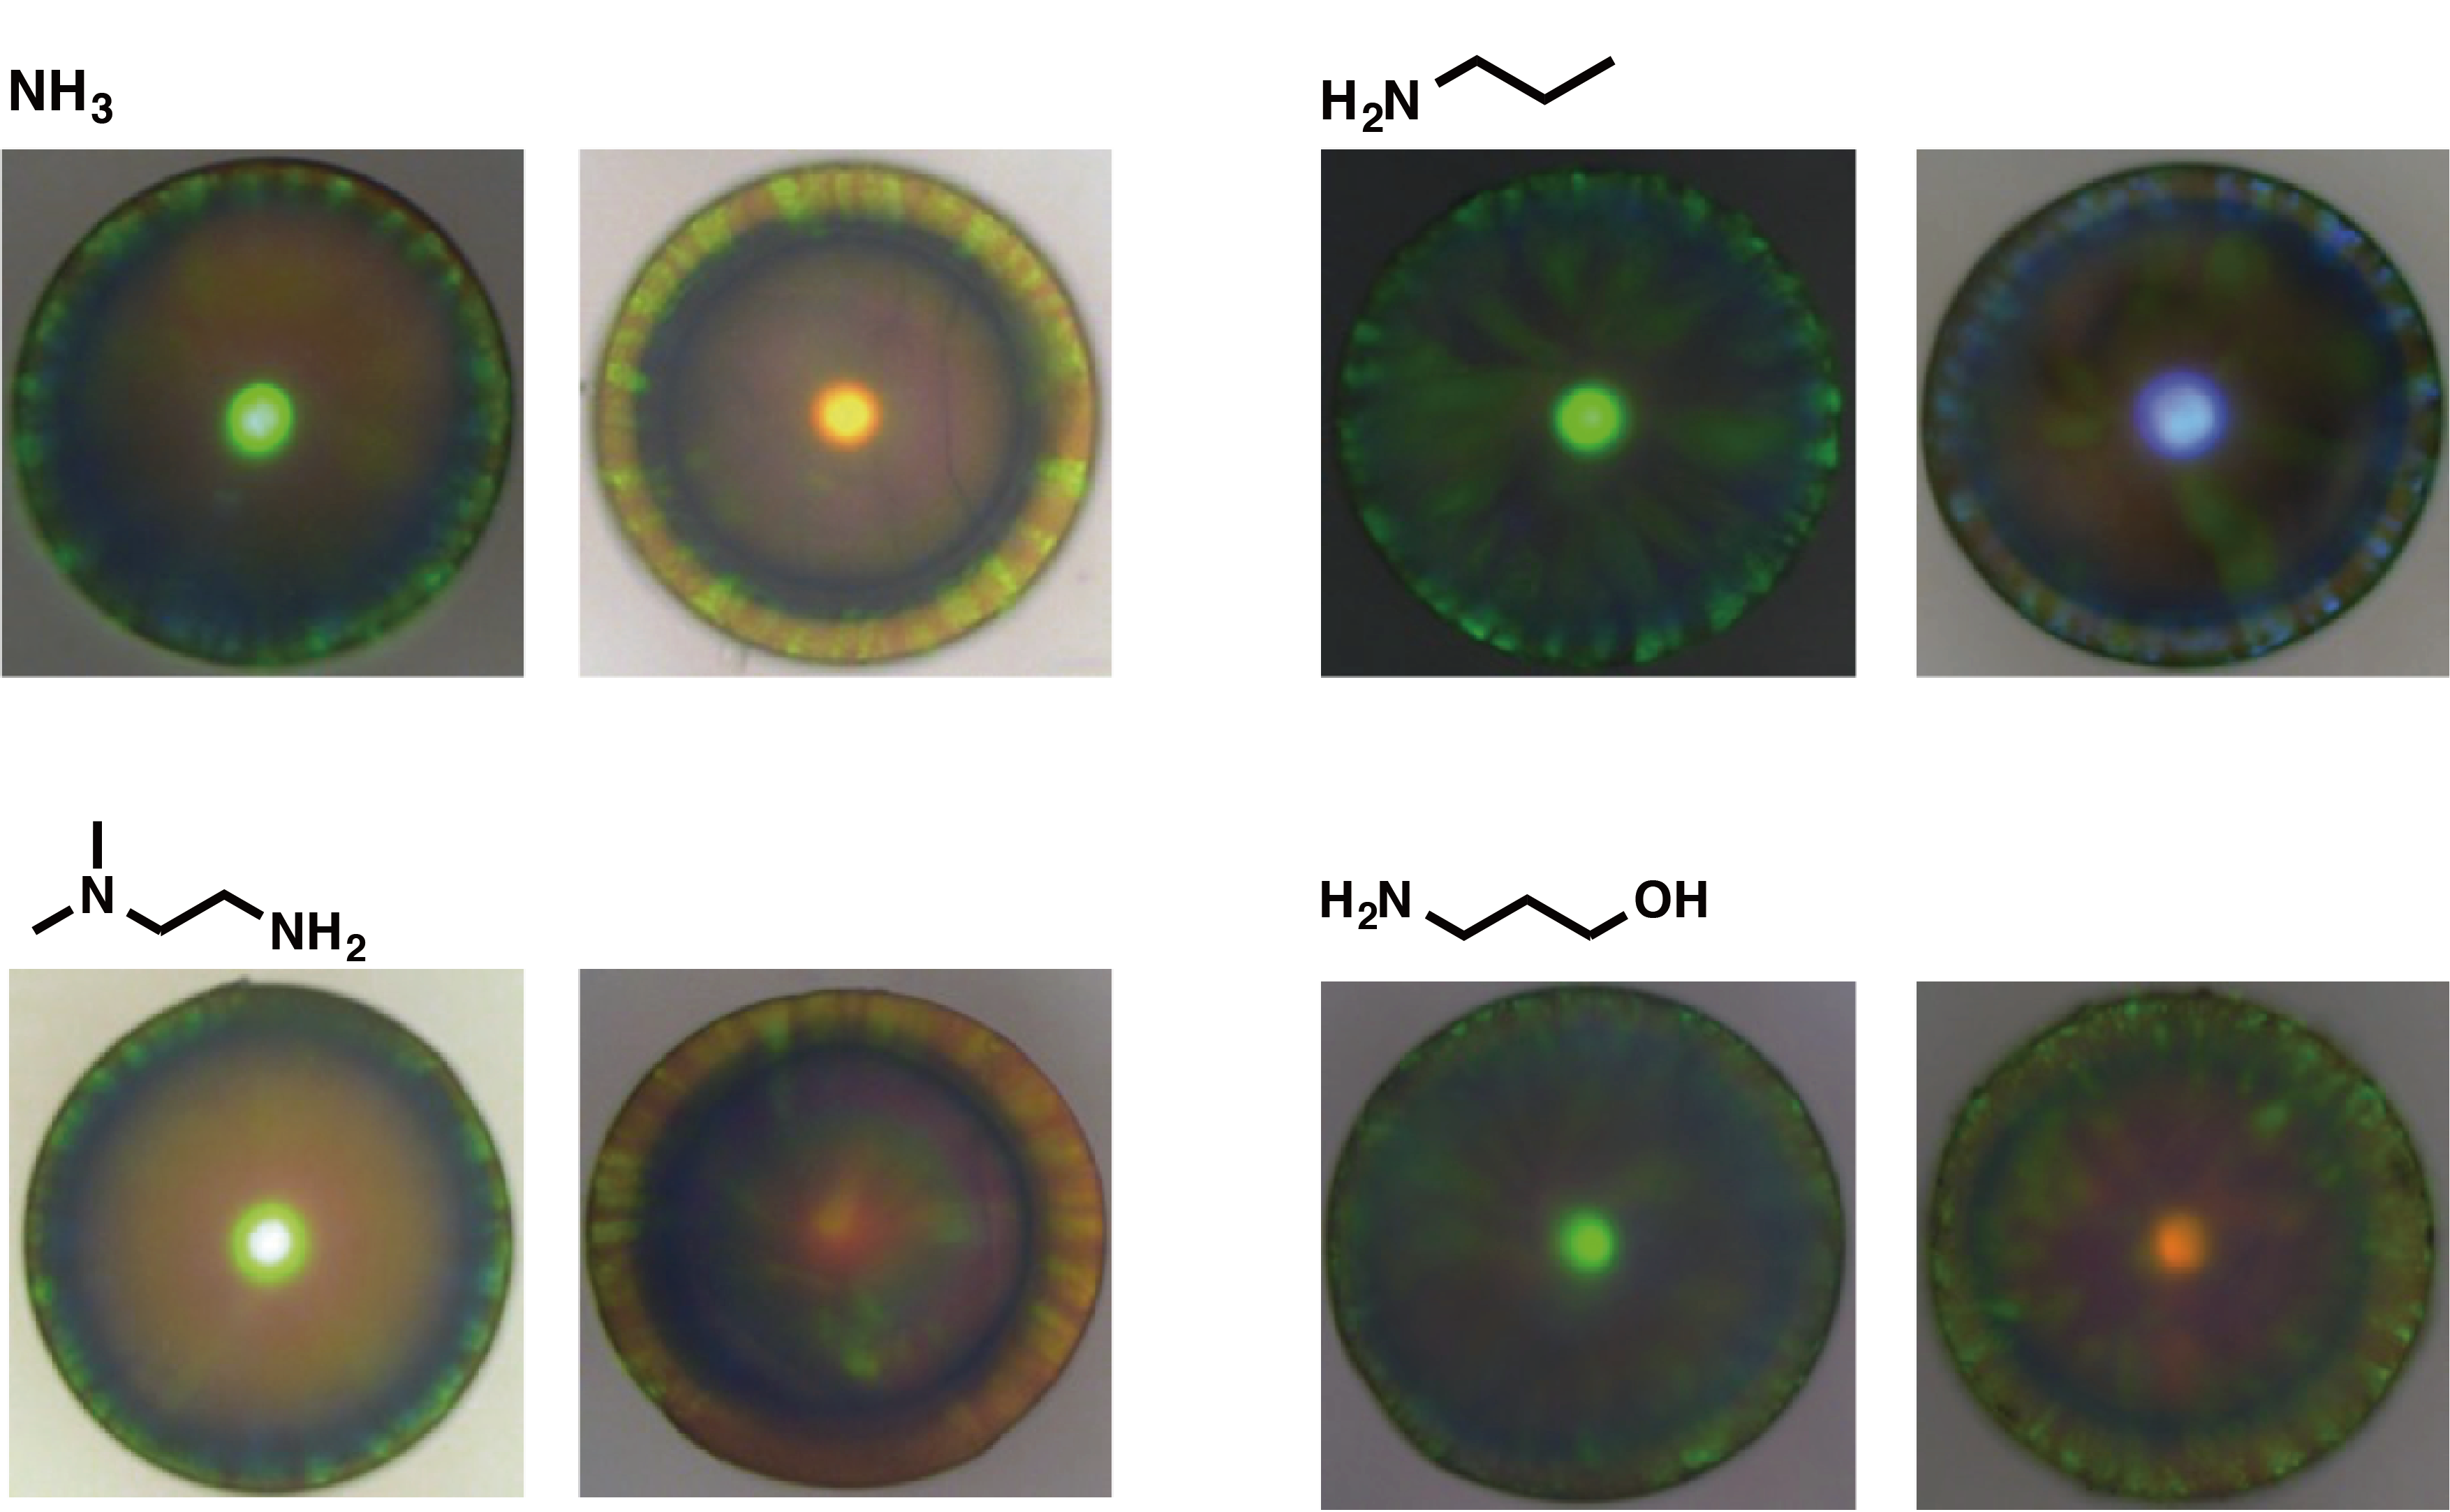
\includegraphics[width=0.9\linewidth]{figures/ch3/CCB-Amine-reaction.png}
    \end{center}
  \end{figure}
\end{frame}

\begin{frame}
  \frametitle{原理验证}
  \begin{figure}
    \begin{center}
      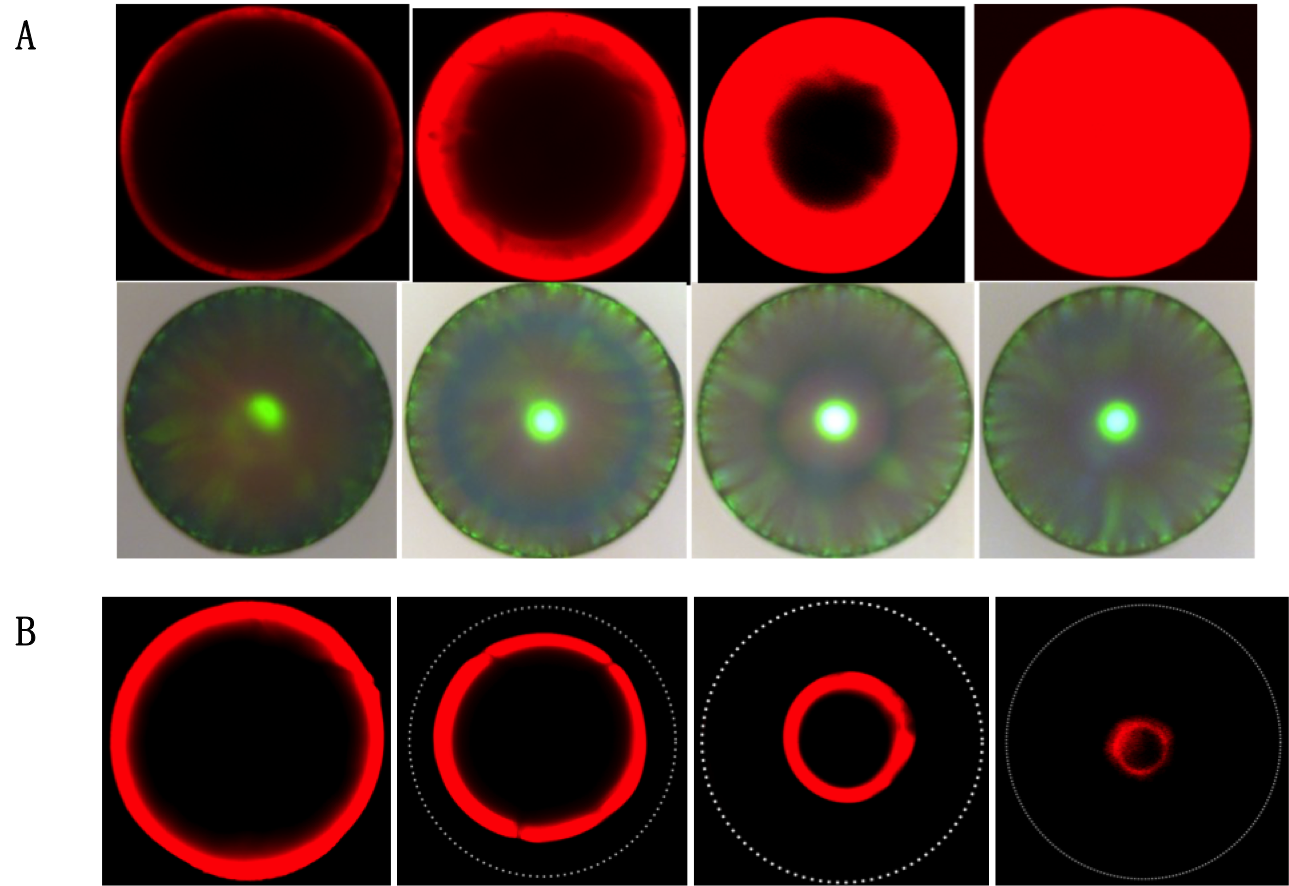
\includegraphics[width=0.8\linewidth]{figures/ch3/Figure2.png}
    \end{center}
  \end{figure}
\end{frame}


\begin{frame}
  \frametitle{三维亲疏水梯度体系}
  \begin{figure}
    \begin{center}
      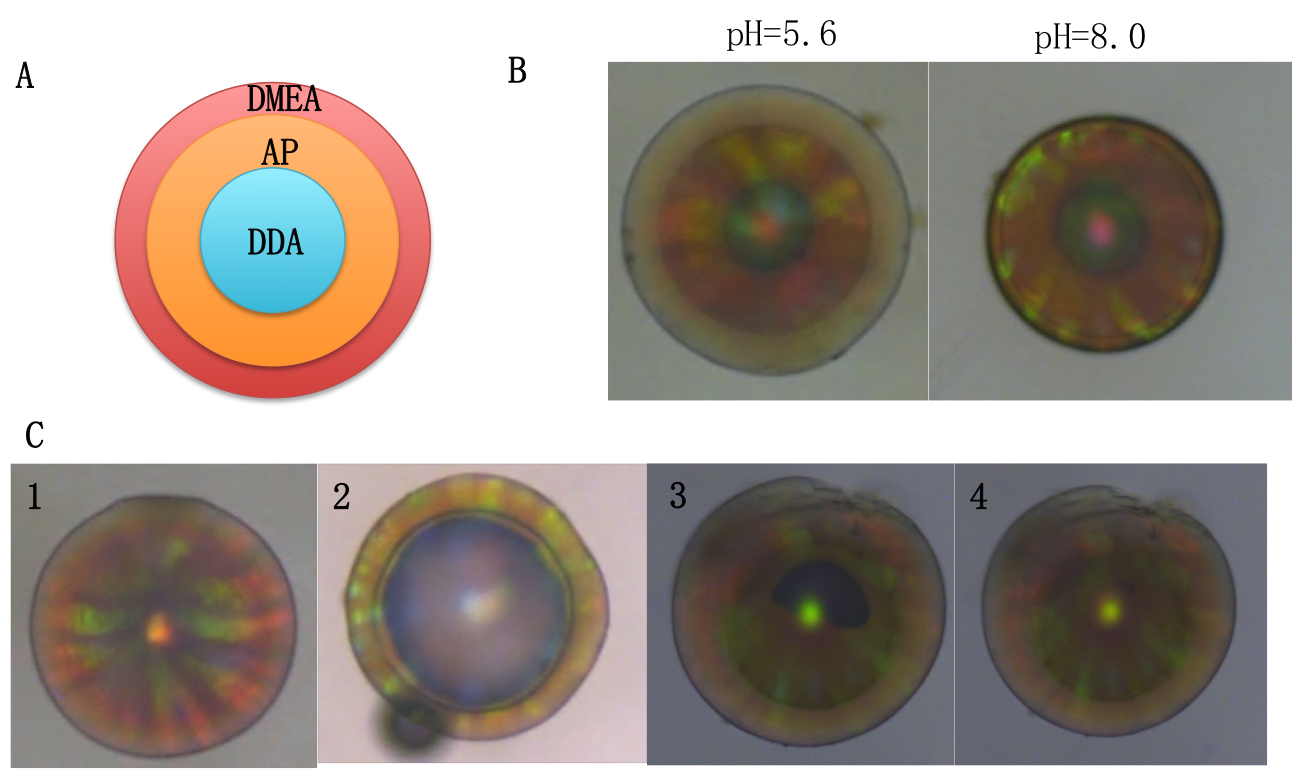
\includegraphics[width=0.9\linewidth]{figures/ch3/Figure3.png}
    \end{center}
  \end{figure}
\end{frame}

\begin{frame}
  \frametitle{正交化学反应微球}
  \begin{figure}
    \begin{center}
      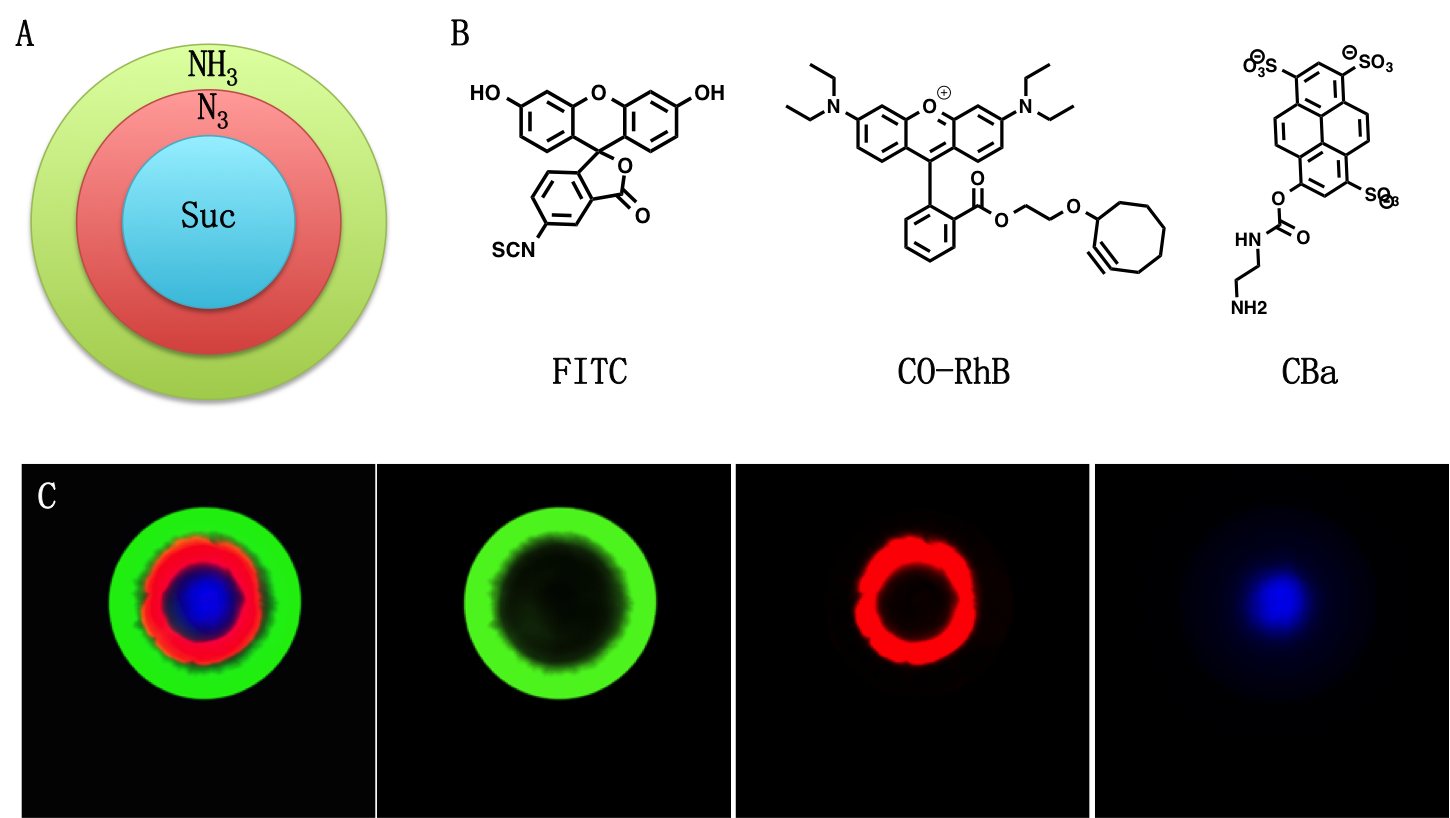
\includegraphics[width=0.9\linewidth]{figures/ch3/Figure4.png}
    \end{center}
  \end{figure}
\end{frame}

\begin{frame}
  \frametitle{自表达级联反应体系}
  \begin{figure}
    \begin{center}
      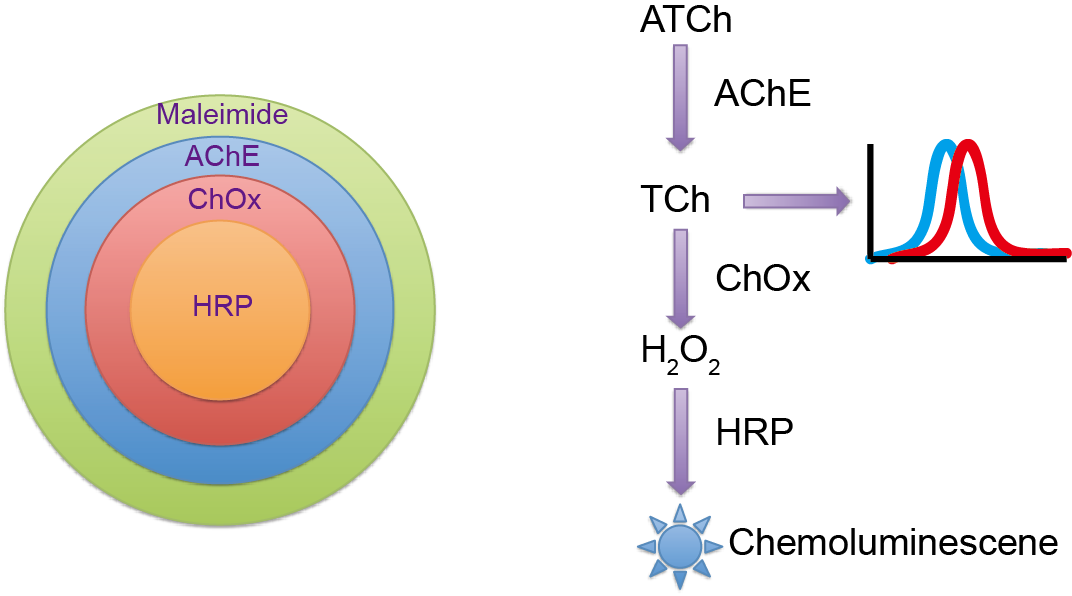
\includegraphics[width=0.8\linewidth]{figures/ch3/cascade.png}
    \end{center}
  \end{figure}
\end{frame}
\begin{frame}
  \frametitle{自表达级联反应体系}
  \begin{figure}
    \begin{center}
      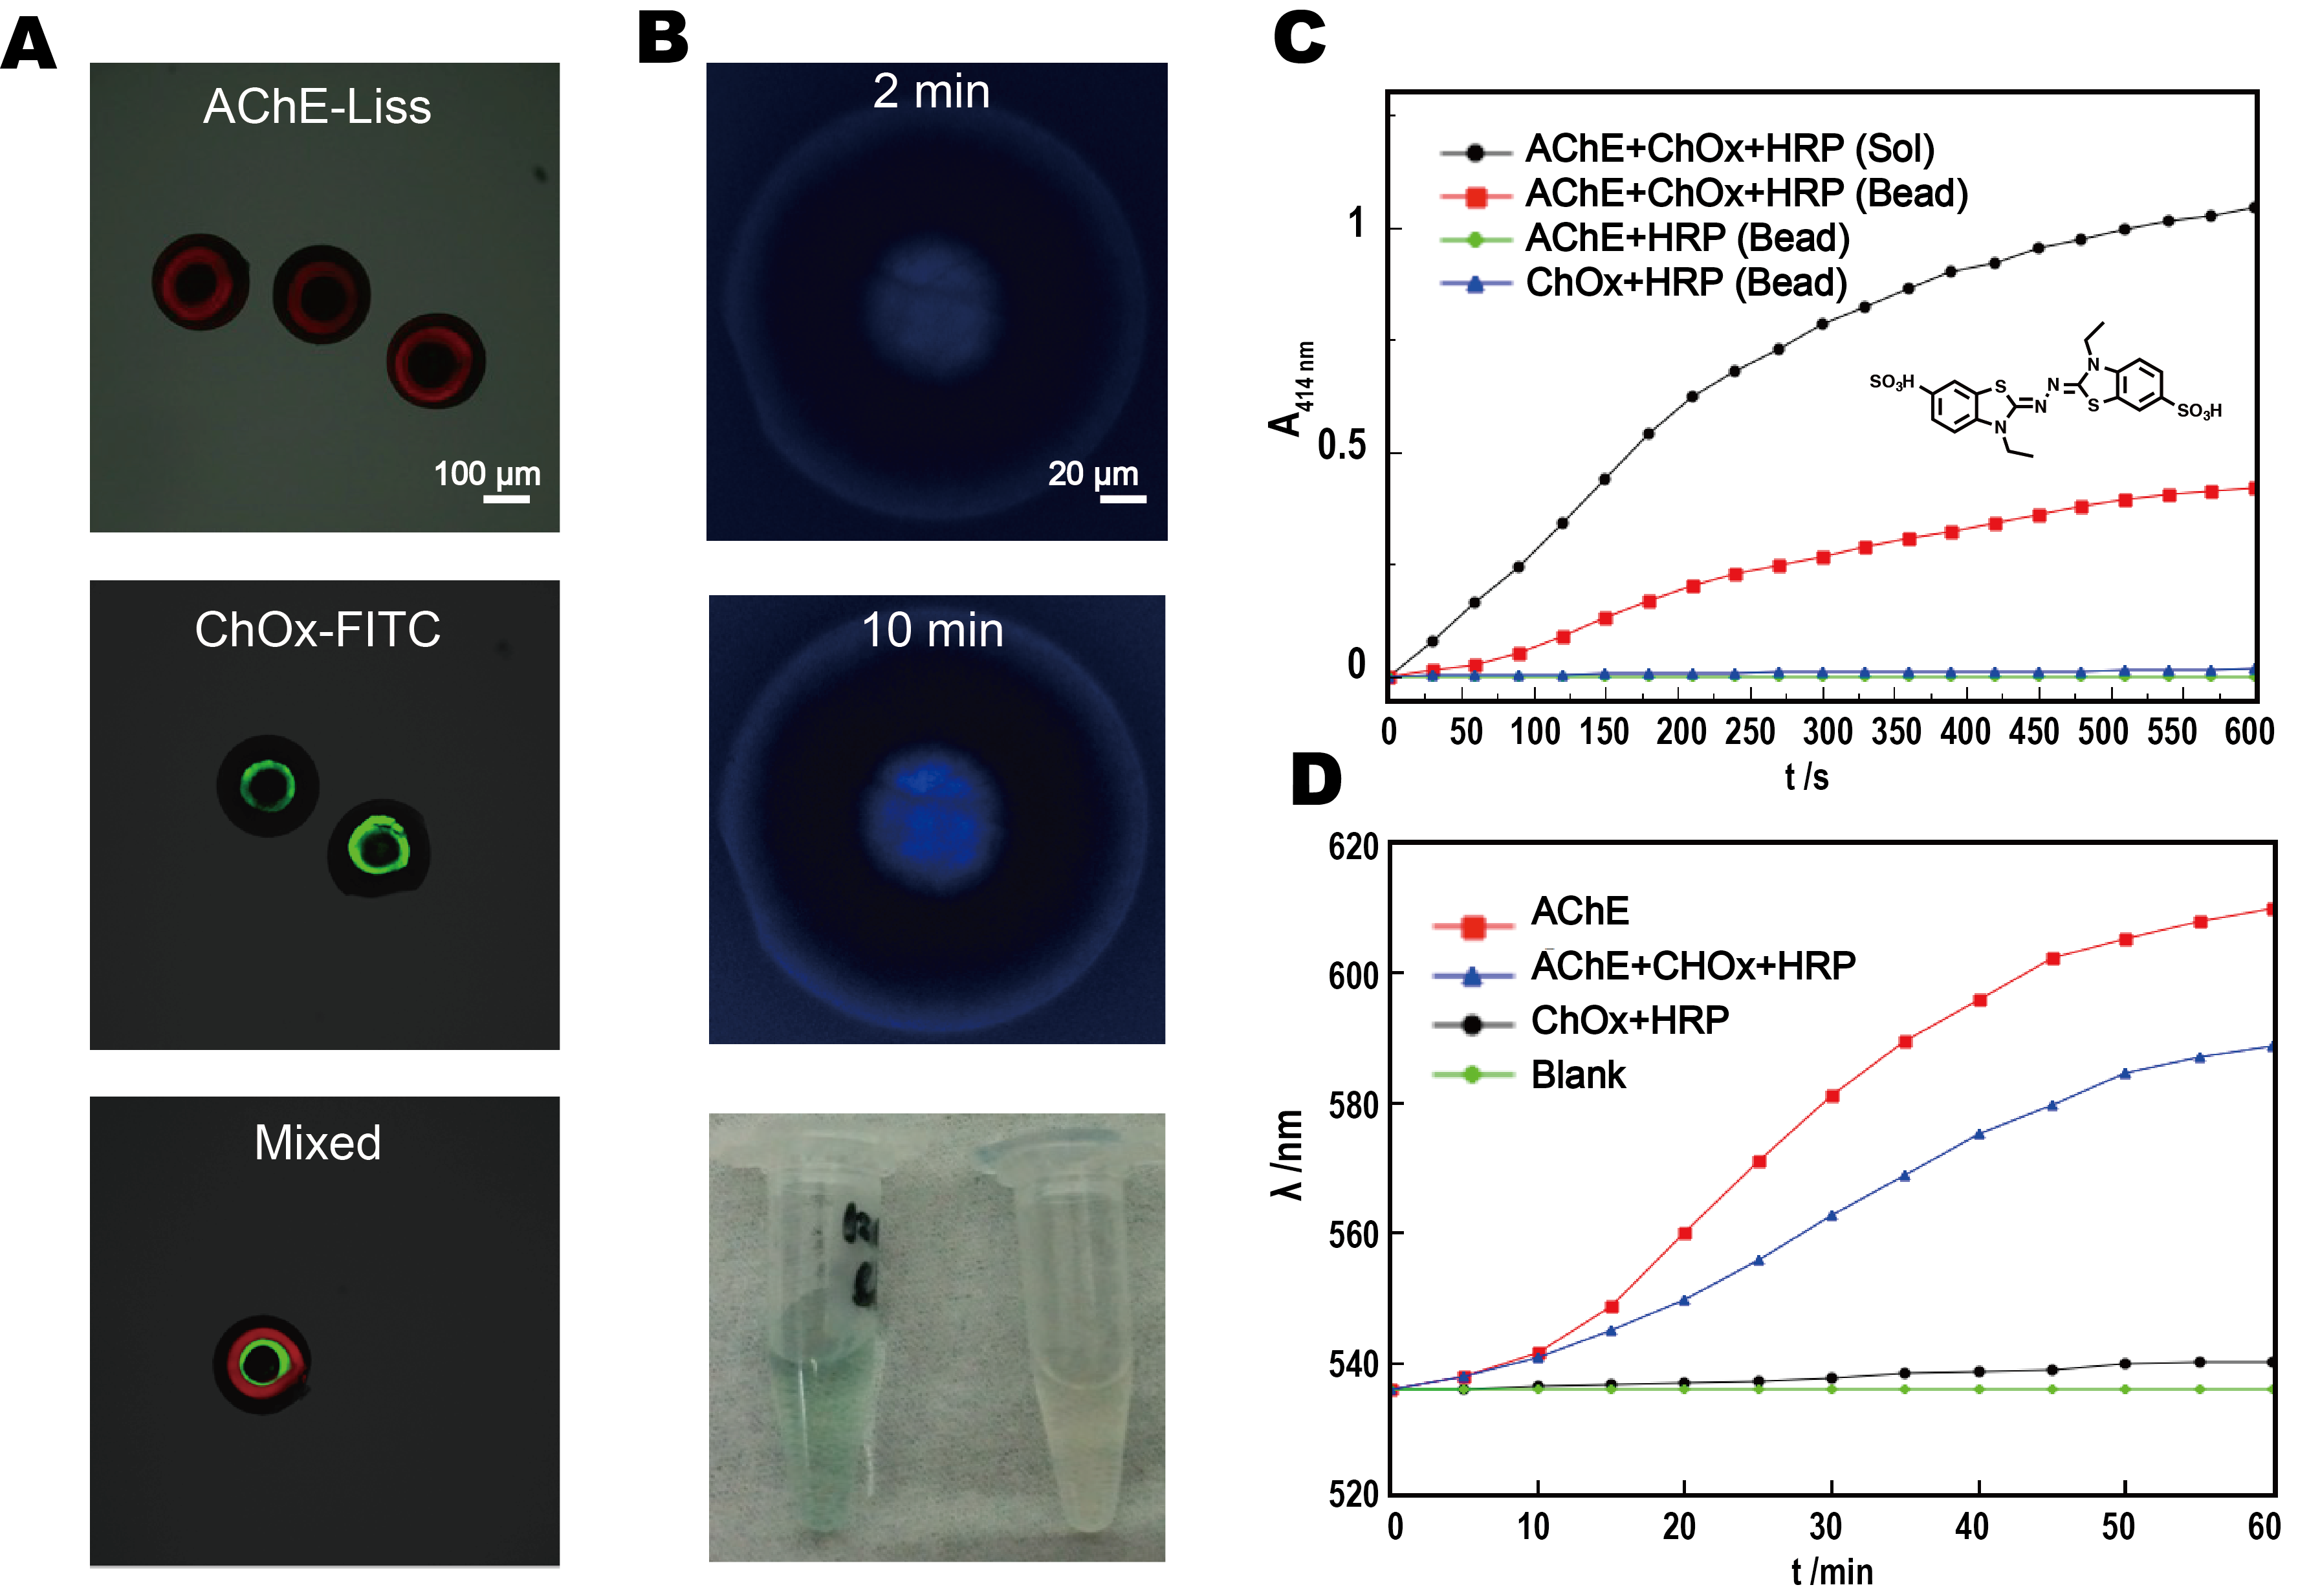
\includegraphics[width=0.85\linewidth]{figures/ch3/cascade-res.png}
    \end{center}
  \end{figure}
\end{frame}

\begin{frame}
  \frametitle{本章小结}
  \begin{itemize}
    \item
    基于选择性刻蚀-反应成功实现了在光子晶体微球上的三维化学修饰与功能化;具有可调节的层数、组分及比例
    \item
    光子晶体光学特性、孔道特性与三维复杂化学组成的有机整合使光子晶体具有极大的拓展性;
    \item
    基于选择性刻蚀-反应实现了三维尺度上的亲疏水梯度、正交化学反应微球、自表达级联反应体系等应用;
  \end{itemize}
\end{frame}

\section{结论}
\begin{frame}
  \frametitle{总结}
  %\begin{itemize}[<+-| alert@+>]
  \begin{itemize}
    \item
    化学反应的多样性赋予了光子晶体材料充分的可调节性与可拓展性;
    \item
    通过马来酰亚胺-巯基反应发展了信号自表达的乙酰胆碱酯酶活性传感光子晶体材料;
    \item
    基于光敏高分子与选择性化学修饰实现了平面反蛋白石光子晶体的图案化与功能化,有利于光子晶体的实际应用;
    \item
    结合选择性刻蚀-反应方法与光子晶体微球,实现了光子晶体材料三维尺度上的功能化;基于光子晶体光学性质、孔洞结构及三维复杂化学组成的协同作用发展了一种可拓展的光子晶体平台。
  \end{itemize}
\end{frame}

\begin{frame}
  \frametitle{在读期间发表的学术论文}
  {
  \begin{enumerate}
  \scriptsize
  \item \textbf{Tian T}, Li X, Cui J, Li J, Lan Y, Wang C, Zhang M, Wang H, Li G. \textit{ACS Appl. Mater.Interfaces}, \textbf{2014}, 6:15456–15465. 
  
  \item Li W, \textbf{Tian T}, Zhu W, Cui J, Ju Y, Li G. \textit{Polym. Chem.}, \textbf{2013}, 4:3057–3068.
  
  \item Yang H, Li X, Lan Y, \textbf{Tian T}, Cui J, Zhu T, Shen D, Li G. \textit{J. Mater. Chem. C}, \textbf{2013}, 1:6120–6128.
  
  \item Xu D, Zhu W, Wang C, \textbf{Tian T}, Li J, Lan Y, Zhang G, Zhang D, Li G. \textit{Chem. Commun.}, \textbf{2014}, 50:14133–14136.
  
  \item Xu D, Zhu W, Wang C, \textbf{Tian T}, Cui J, Li J, Wang H, Li G. \textit{Chem. Eur. J.}, \textbf{2014}, 20:16620-16625.
  
  \item Zhu T, Xu D, Wu Y, Li J, Zhou M, \textbf{Tian T}, Jiang Y, Li F, Li G. \textit{J. Mater. Chem. B}, \textbf{2013}, 1:6449–6458.
  
  \item Wang C, Zhu W, Lan Y, Zhang M, \textbf{Tian T}, Wang H, Li G. \textit{J. Phys. Chem. C}, \textbf{2014}, 118:10754–10763.

  \end{enumerate}
  }
\end{frame}

\begin{frame}
  \frametitle{致谢}
  \begin{itemize}
    \item
    感谢我的导师李广涛教授在基础知识、科研素养、科研洞察力上对我的悉心指导!他的培养使我终身收益。
    \item
    感谢实验室全体同仁在平时实验及科研交流方面给予我的无私帮助!
    \item
    感谢我的家人在平时对我的生活与学习上的帮助!
    \item
    感谢国家自然科学基金及中德重大合作项目(TRR61)的资金支持,特此致谢!
  \end{itemize}
\end{frame}

\begin{frame}
  \begin{figure}[htbp]
    \centering
    
\includegraphics[width=0.5\linewidth]{figures/thankyou.png}
  \end{figure}
\end{frame}

\begin{frame}
  \frametitle{马来酰亚胺聚合物光子晶体接触角测试}
  \begin{figure}[htbp]
    \centering
    \includegraphics[width=0.30\linewidth]{figures/Maleimide-CA.png}
  \end{figure} 
\end{frame}

\begin{frame}
  \frametitle{光敏功能单体合成与机理}
  \begin{figure}[htbp]
    \centering
    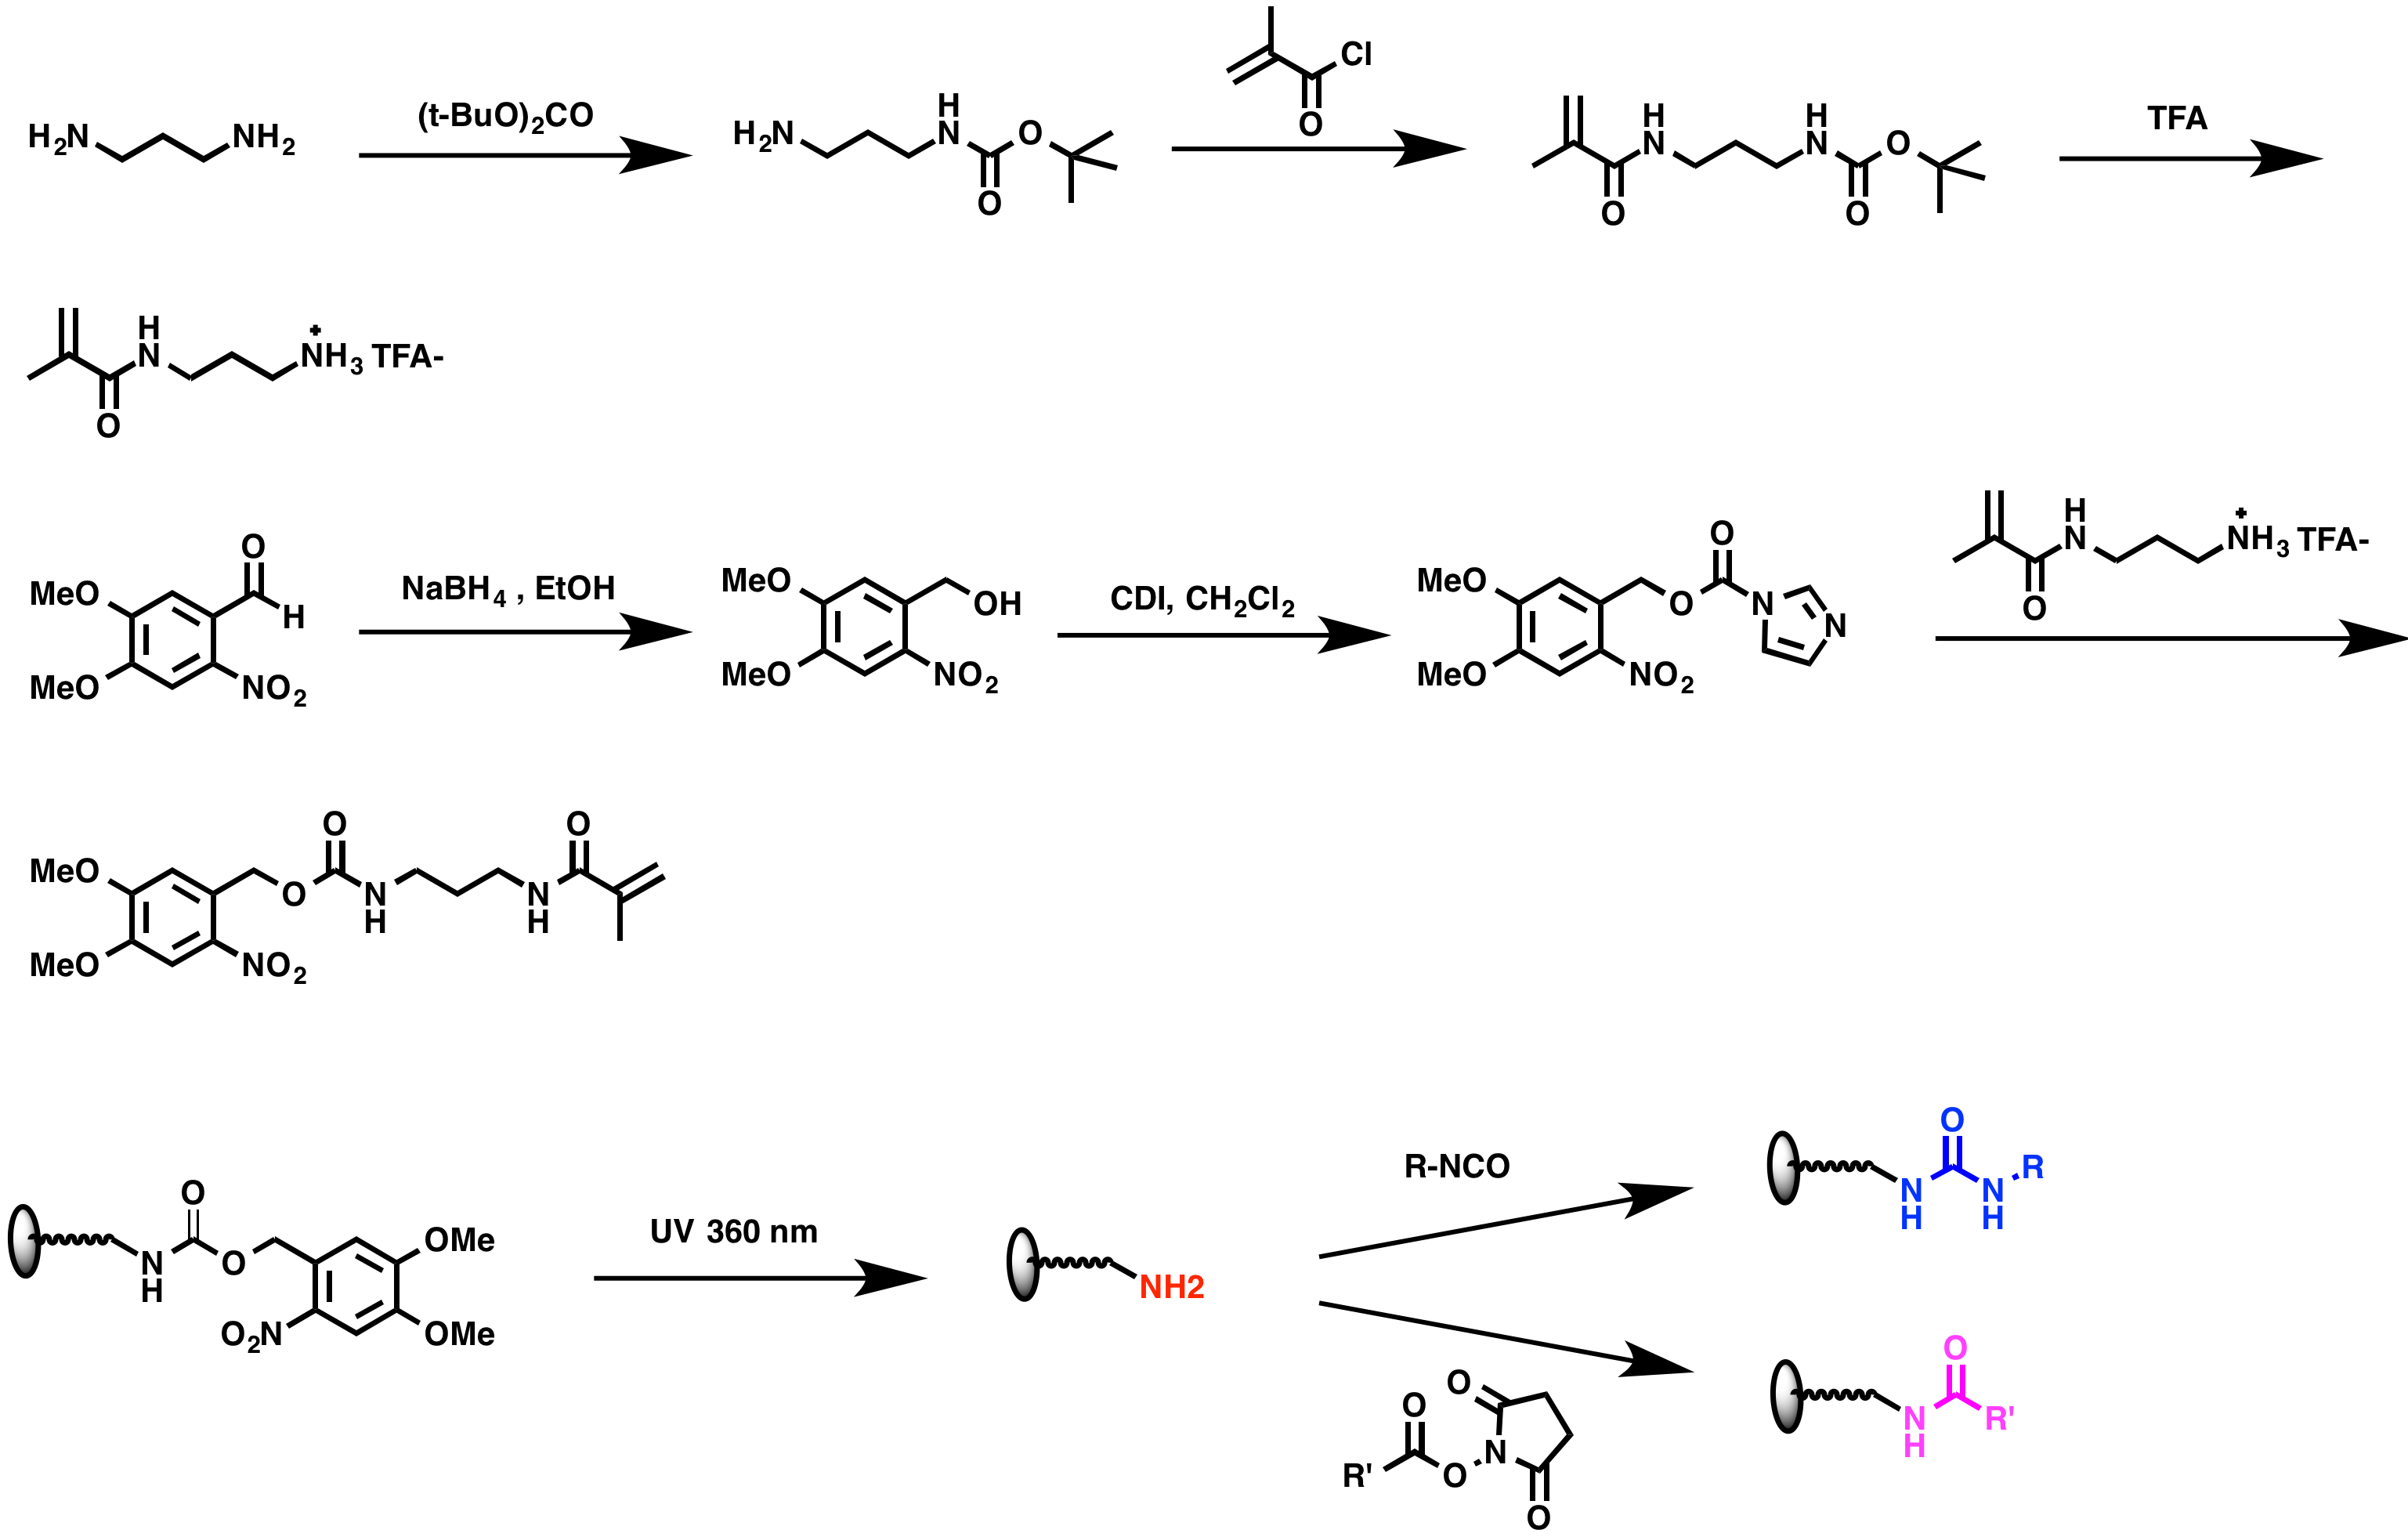
\includegraphics[width=0.95\linewidth]{figures/scheme-NVOC.png}
  \end{figure} 
\end{frame}

\begin{frame}
  \frametitle{光子晶体微球刻蚀过程}
  \begin{figure}
    \begin{center}
      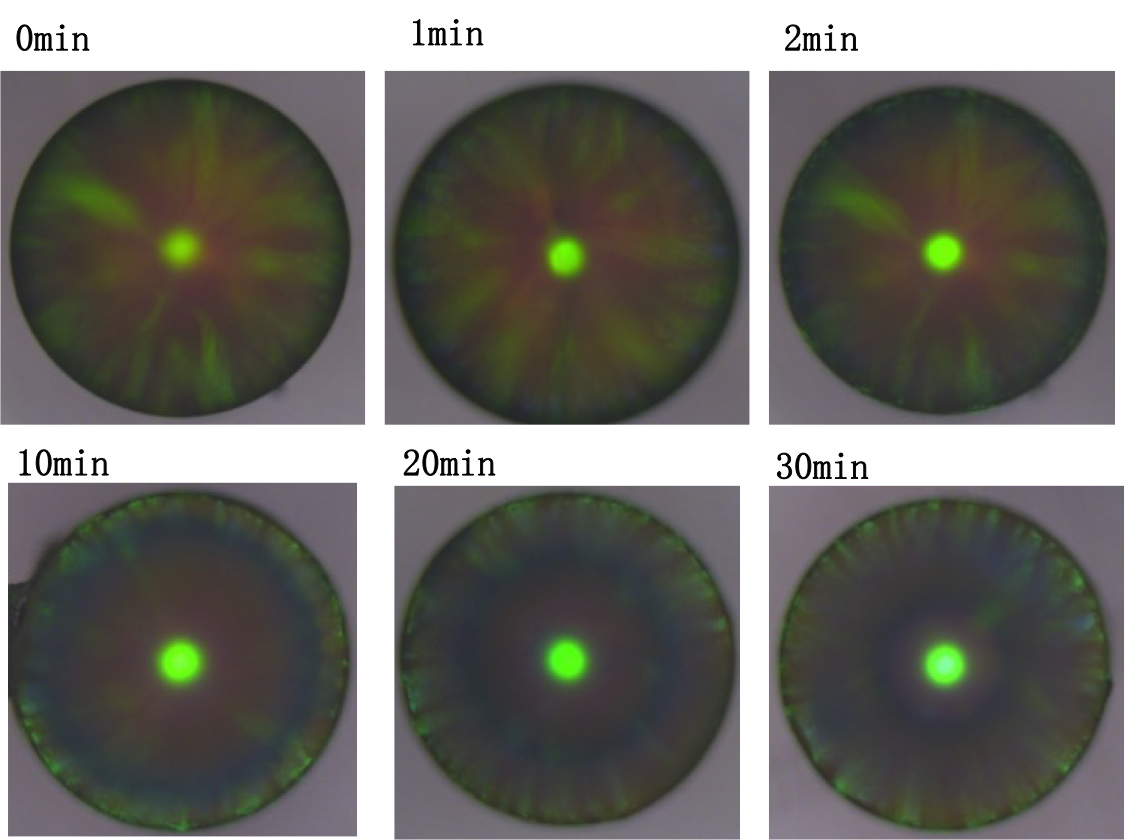
\includegraphics[width=0.8\linewidth]{figures/ch3/Fig1A.png}
    \end{center}
  \end{figure}
\end{frame}

\begin{frame}
  \frametitle{光子晶体微球修饰-IR证明}
  \begin{figure}
    \begin{center}
      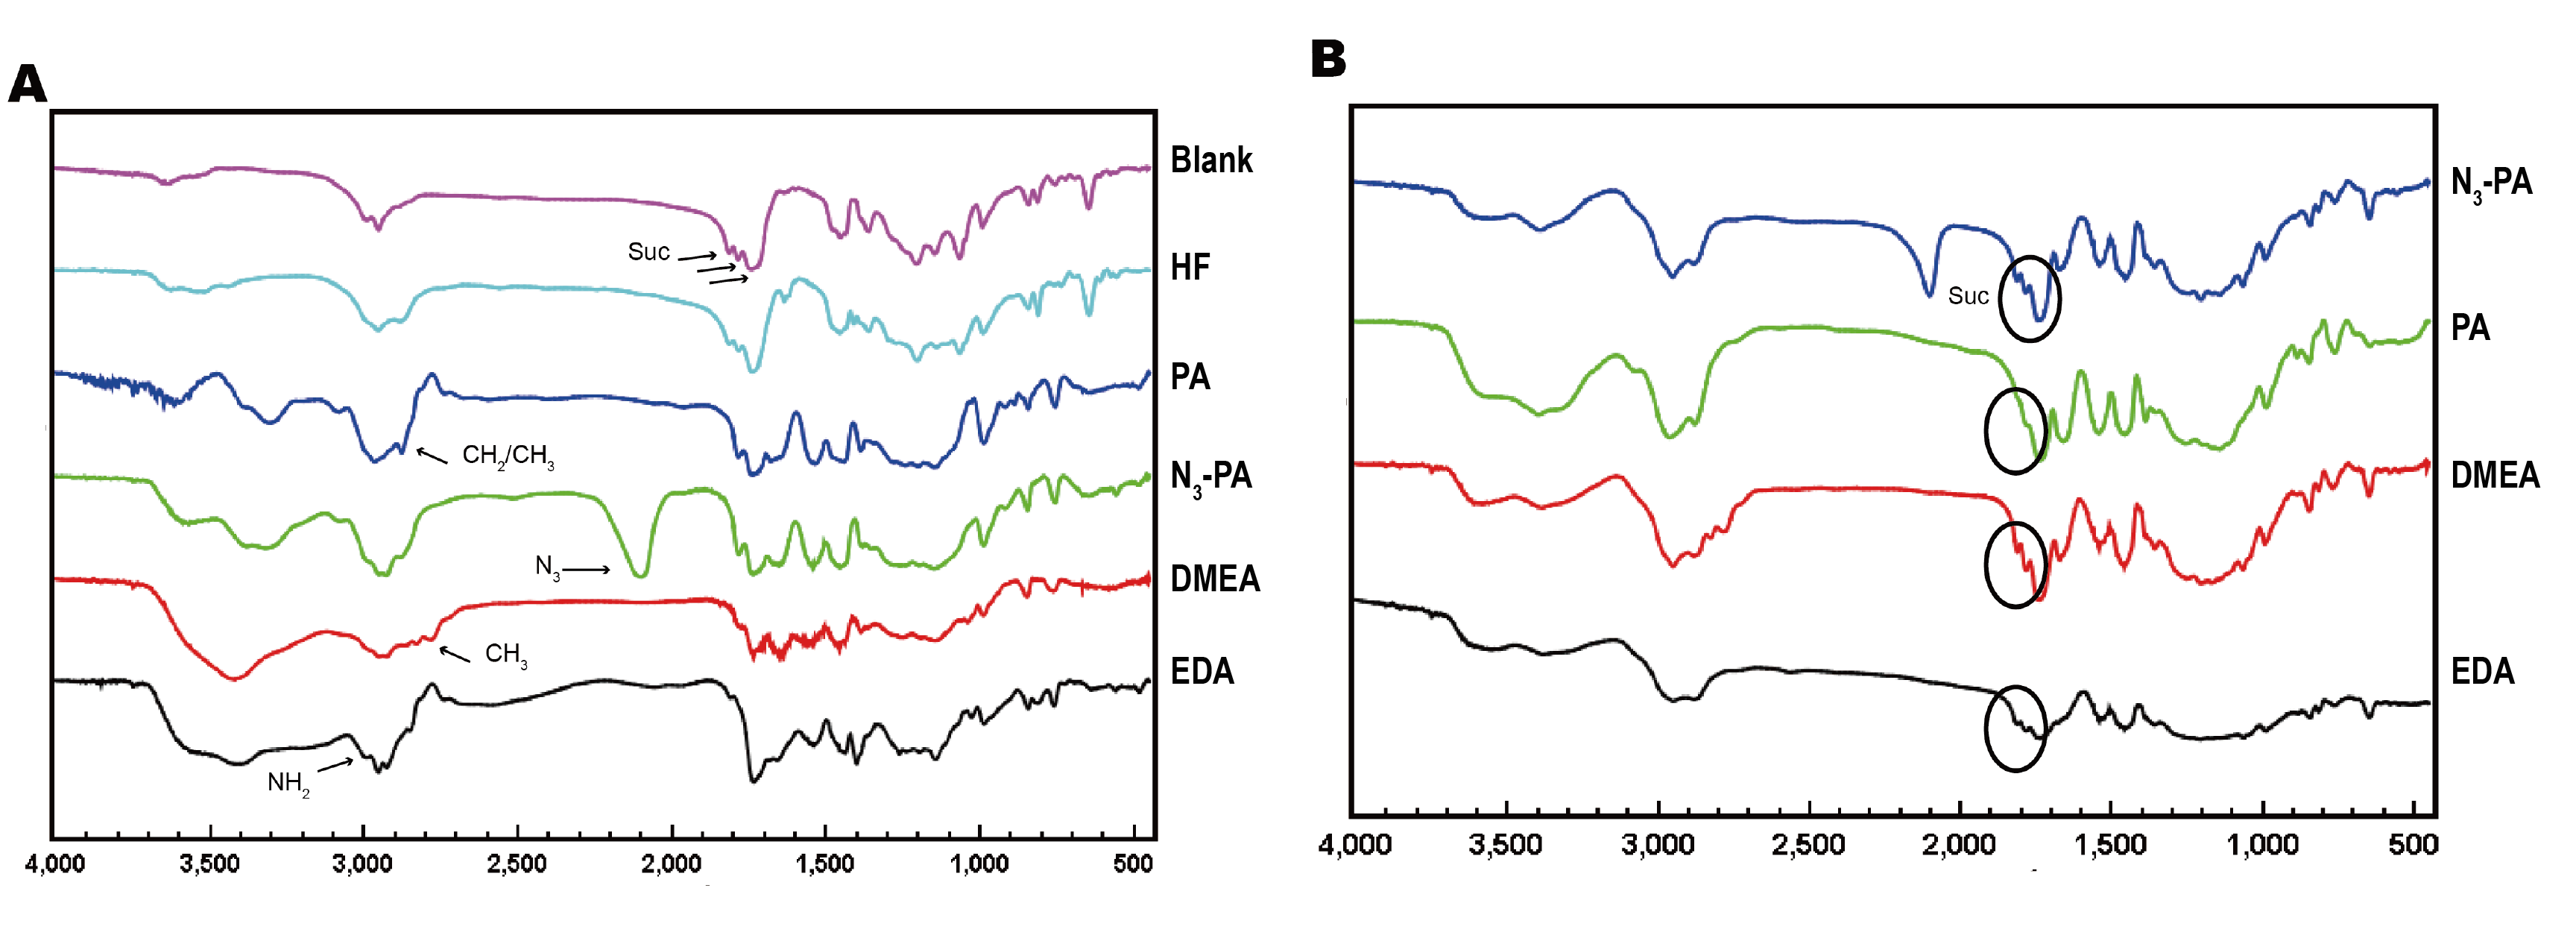
\includegraphics[width=\linewidth]{figures/ch3/IR.png}
    \end{center}
  \end{figure}
\end{frame}

\begin{frame}
  \frametitle{三维亲疏水梯度体系-接触角实验}
  \begin{figure}
    \begin{center}
      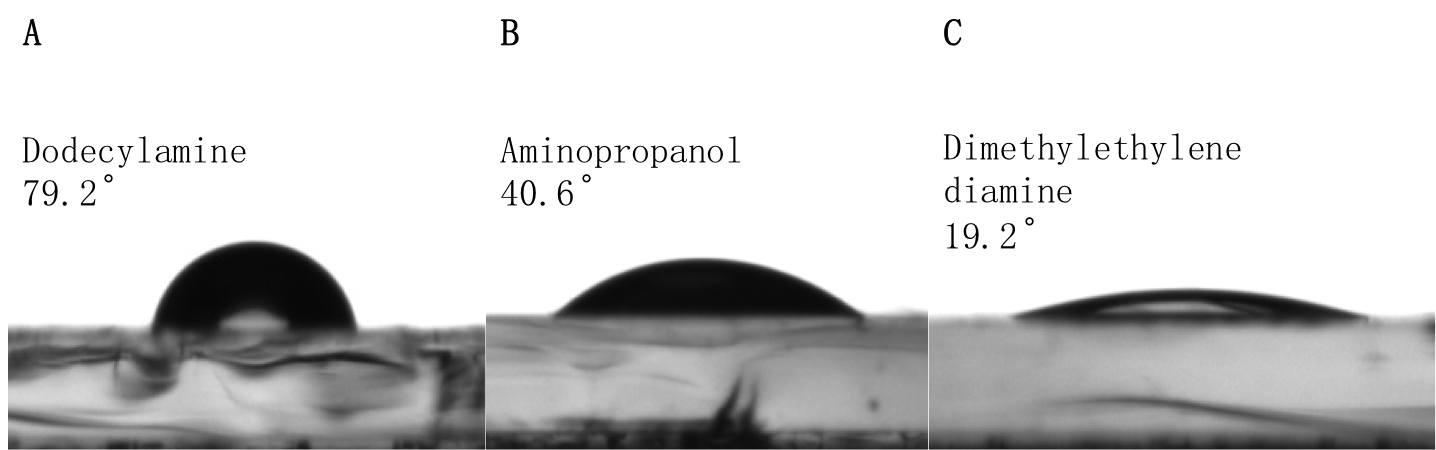
\includegraphics[width=\linewidth]{figures/ch3/FigureS3.png}
    \end{center}
  \end{figure}
\end{frame}

\begin{frame}
  \frametitle{正交化学反应微球-原位CLMS}
  \begin{figure}
    \begin{center}
      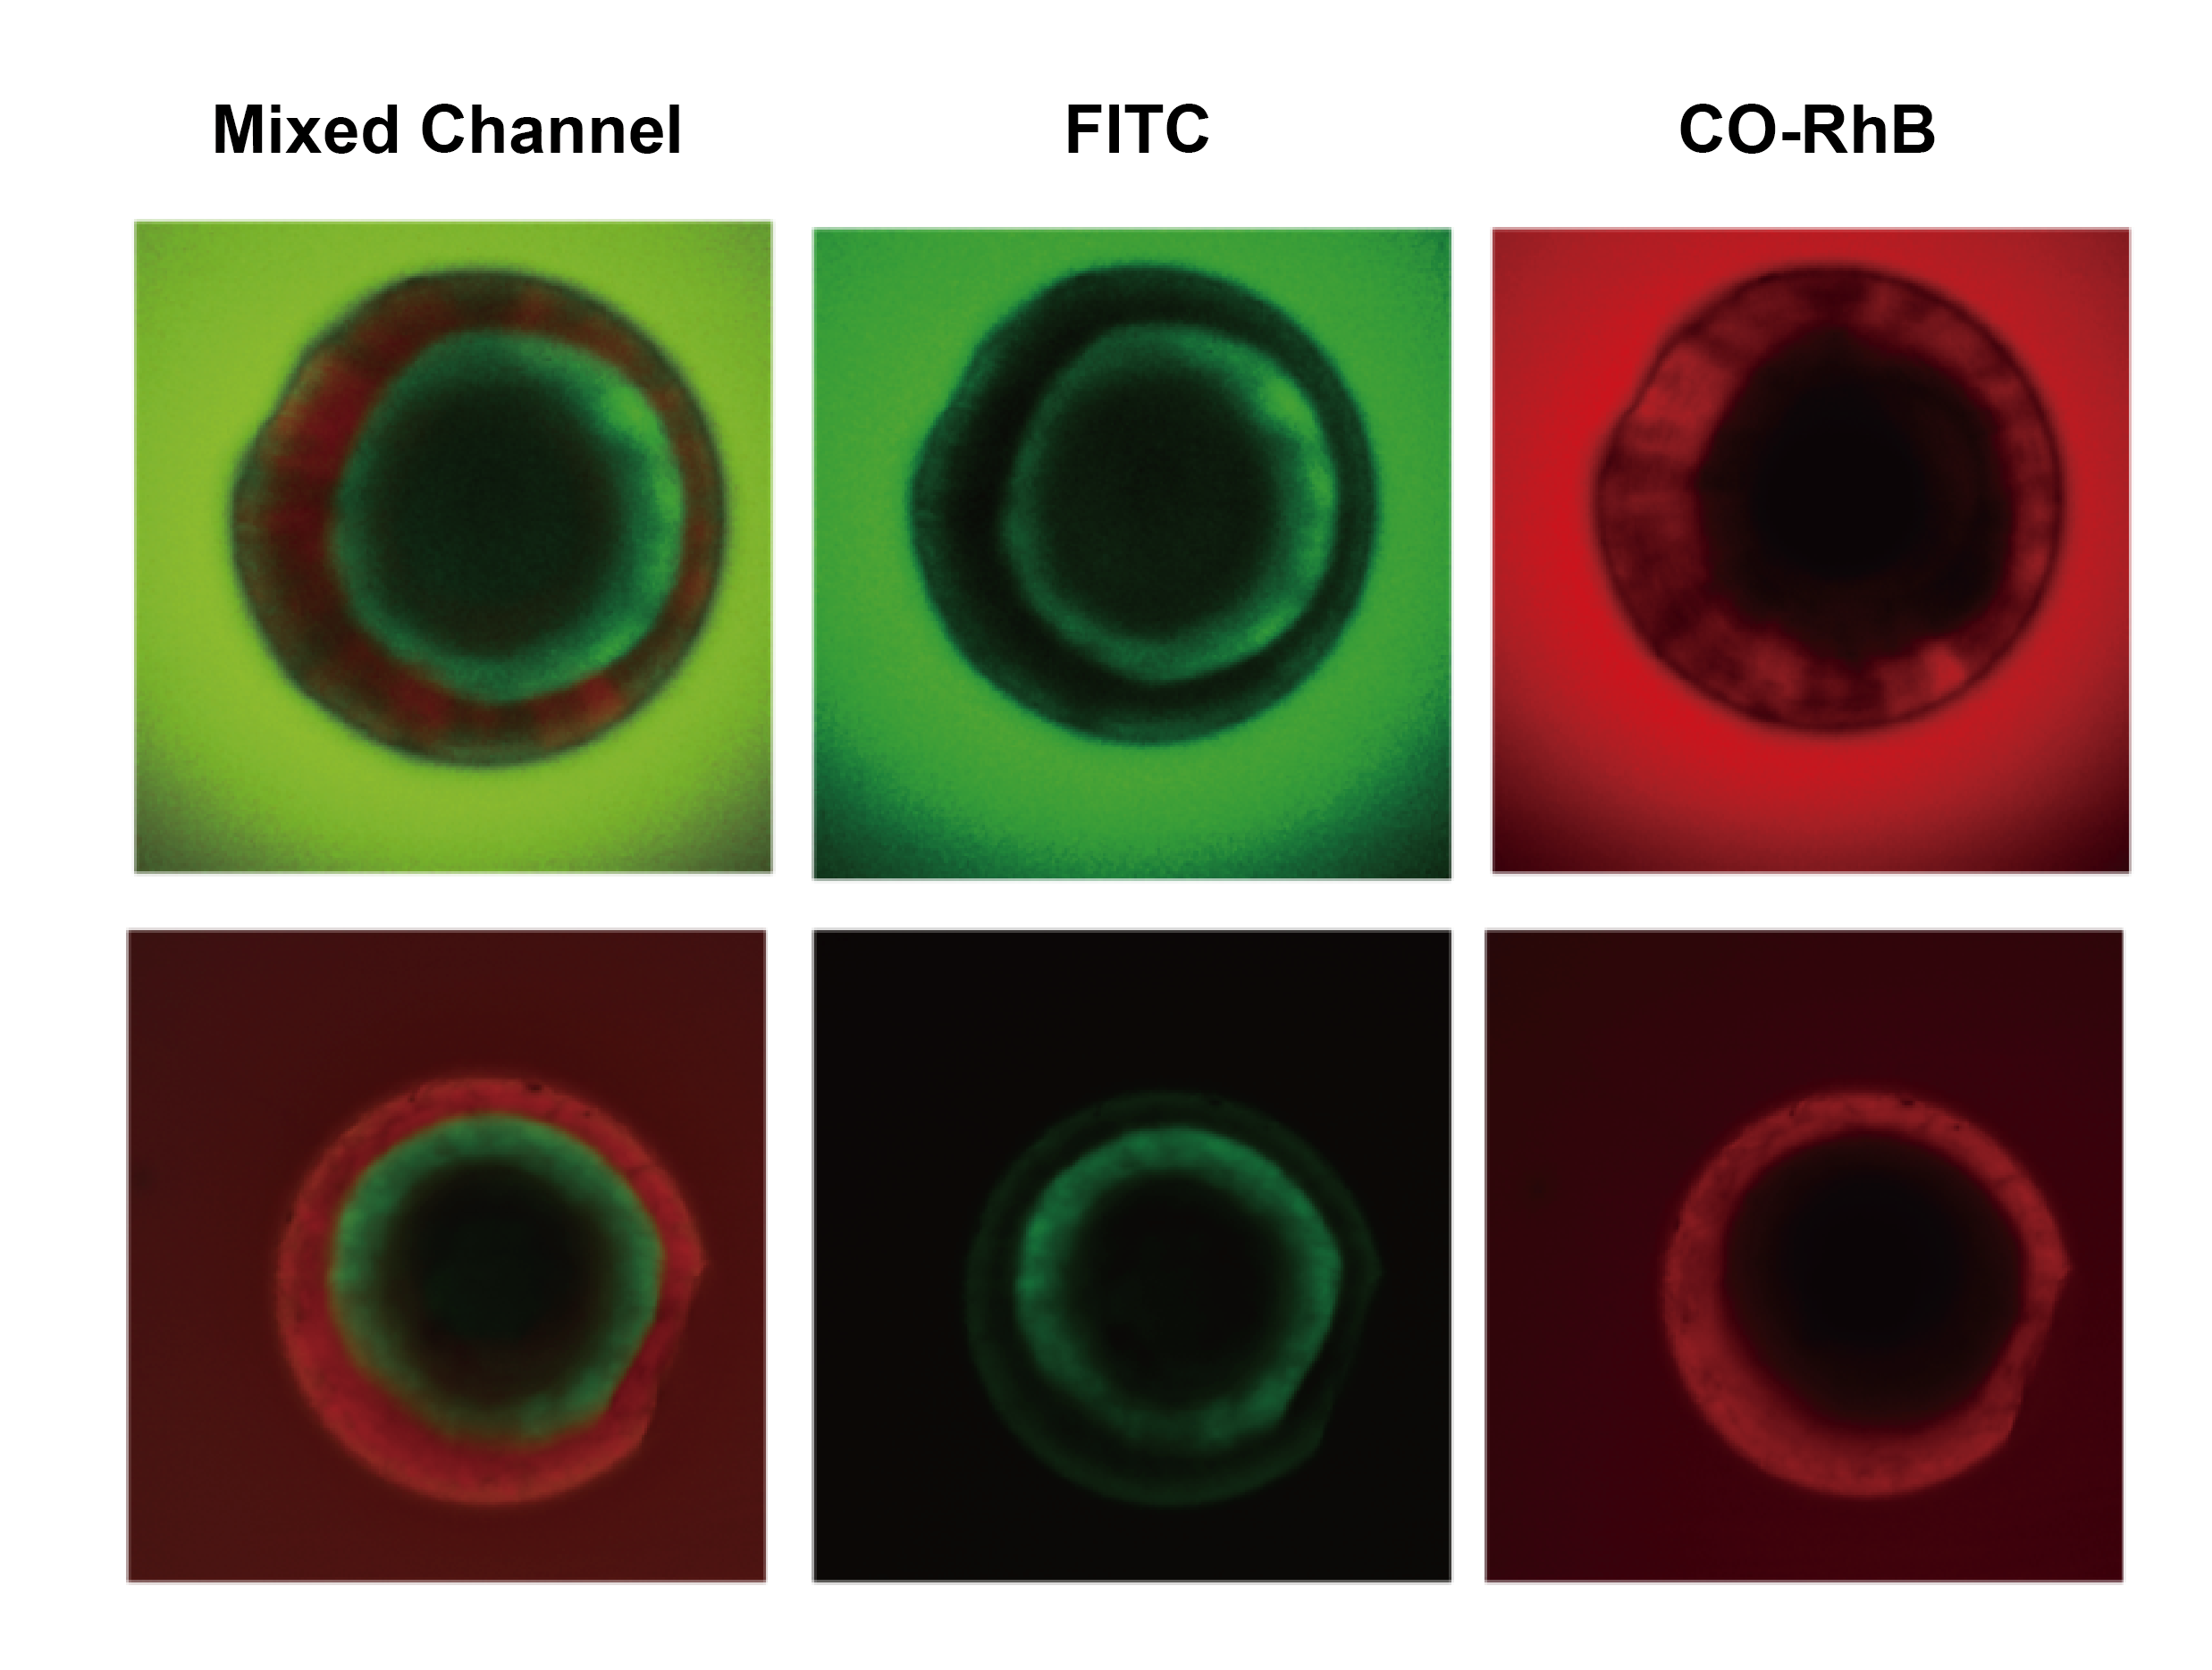
\includegraphics[width=0.8\linewidth]{figures/ch3/dualstain.png}
    \end{center}
  \end{figure}
\end{frame}

\end{document}